\documentclass[11pt,a4paper,twoside,openright]{memoir}

% Essential packages
\usepackage{calc,url,fancyvrb}
\usepackage{multicol,keyval}
\usepackage{graphicx,color}
\graphicspath{{img/}}
%\usepackage[scale = 0.75]{geometry}
\usepackage[left=3cm,top=3cm,right=2cm,bottom=3cm]{geometry}
%\usepackage[left=1.5in, right=1in, top=1in, bottom=1in, includefoot, headheight=13.6pt]{geometry}
\usepackage[square, comma, numbers, sort&compress]{natbib}
%\usepackage[T1]{fontenc}
%\usepackage[draft]{fixme}
\usepackage[adobe-utopia]{mathdesign}
%\usepackage{times}
\usepackage[scaled]{luximono}
%\newcommand\starbreak{\fancybreak{\decosix\quad\decosix\quad\decosix}}
\usepackage[scaled]{berasans}
\usepackage[italian]{babel}
\usepackage{indentfirst}
%\usepackage{mathptmx}
\usepackage[nice]{nicefrac}
\usepackage{textcomp} % risolve \textdegree per memoir.cls
%\usepackage{fixfoot}
%\usepackage{subfigure}
%\usepackage{float} % anche per inserire codice formattato con verbatim



%\long\def\symbolfootnote[#1]#2{\begingroup%
%\def\thefootnote{\fnsymbol{footnote}}\footnote[#1]{#2}\endgroup}

% Optional customisation packages
%\usepackage{mathpazo}
%\usepackage[hang, small, bf, margin=20pt, tableposition=top]{caption} 
%\setlength{\abovecaptionskip}{10pt}

%\renewcommand{\footnoterule}
%\setlength{\footmarkwidth}{-1.0em}
%\setlength{\footmarksep}{-\footmarkwidth}
%\footmarkstyle{#1}

%\usepackage{endnotes}
%\renewcommand{\footnote}{\endnote}
%\renewcommand{\enotesize}{\normalsize}



\usepackage{soul}
\definecolor{royalblue}{rgb}{.200,.400,.600}
\definecolor{gray}{rgb}{.200,.200,.200}

\makeatletter
\newlength\dlf@normtxtw
\setlength\dlf@normtxtw{\textwidth}
\def\myhelvetfont{\def\sfdefault{mdput}}
\newsavebox{\feline@chapter}
\newcommand\feline@chapter@marker[1][4cm]{%
\sbox\feline@chapter{%
\resizebox{!}{#1}{\fboxsep=1pt%
\colorbox{royalblue}{\color{white}\bfseries\rmfamily\thechapter}%
}}%
%% inizio scritta capitolo
\rotatebox{90}{%
\resizebox{%
\heightof{\usebox{\feline@chapter}}+\depthof{\usebox{\feline@chapter}}}%
{!}{\scshape\so\@chapapp}}
\quad%
%% fine scritta capitolo
\raisebox{\depthof{\usebox{\feline@chapter}}}{\usebox{\feline@chapter}}%
}
\newcommand\feline@chm[1][4cm]{%
\sbox\feline@chapter{\feline@chapter@marker[#1]}%
\makebox[0pt][l]{% aka \rlap
\makebox[1cm][r]{\usebox\feline@chapter}%
}}
\makechapterstyle{ntilo}{
\renewcommand\chapnamefont{\normalfont\Large\scshape\raggedright\so}
\renewcommand\chaptitlefont{\normalfont\huge\bfseries\scshape\color{royalblue}}
\renewcommand\chapternamenum{}
\renewcommand\printchaptername{}
\renewcommand\printchapternum{\null\hfill\feline@chm[2.5cm]\par}
\renewcommand\afterchapternum{\par\vskip\midchapskip}
\renewcommand\printchaptertitle[1]{\chaptitlefont\raggedright ##1\par}
}
\makeatother
\chapterstyle{ntilo}

% Page layout
%\parindent 0pt
\parskip 1ex
\renewcommand{\baselinestretch}{1.2}
%\numberwithin{equation}{section}
\renewcommand{\bibname}{Bibliografia}
\renewcommand{\contentsname}{Indice}
\pagenumbering{roman}
\bibliographystyle{unsrtnat}

%% MY COMMANDS
%\renewcommand{\footnote}[1]{\textcolor{royalblue}{\footnotemark}\footnotetext{#1}}

\newcommand{\itt}[1]{\textit{#1}}
\newcommand{\marm}[1]{\mathrm{#1}}

\hyphenation{bit-stream}

\renewcommand{\theequation}{\thesection.\arabic{equation}}
%\renewcommand{\thesection}{\arabic{section}}
%\renewcommand{\thesubsection}{(\arabic{subsection})}
%\renewcommand{\thesubsubsection}{(\arabic{subsubsection})}
\setcounter{tocdepth}{2}
\setcounter{secnumdepth}{3}
\setcounter{section}{0}
%\setcounter{figure}{0}

\renewcommand\thefigure{\arabic{figure}}

% Customising chapter headings (optional) - see sectsty.pdf
%\usepackage{sectsty}
%\chapterfont{\large\sc\centering}
%\chaptertitlefont{\centering}
%\subsubsectionfont{\centering}

\makeatletter

\newcounter{Hfootnote}
\let\H@@footnotetext\@footnotetext
\let\H@@footnotemark\@footnotemark

\long\def\@footnotetext#1{%
  \H@@footnotetext{%
%  \hyper@@anchor{\@currentHref}{\relax}{#1} %{#1\vskip 10pt}
  \Hy@raisedlink{\hyper@anchorstart{\@currentHref}\hyper@anchorend}{#1}% Inalza il link a pi� di pagina
 }%
}
\def\@footnotemark{%
  \leavevmode
  \ifhmode\edef\@x@sf{\the\spacefactor}\nobreak\fi
  \H@refstepcounter{Hfootnote}%
  \hyper@makecurrent{Hfootnote}%
  \hyper@linkstart{link}{\@currentHref}%
  \@makefnmark
  \hyper@linkend
  \ifhmode\spacefactor\@x@sf\fi
  \relax
}

\def\addhyperlinkline#1#2{%
  \global\advance\OddToc by 1
  % If we're in vmode we want to revert to vmode
  \edef\@tempa{\ifvmode\vskip0pt\fi}%
  \Hy@raisedlink{\hyper@@anchor{toc\the\OddToc}{\relax}\@tempa}%
  \@writetorep{}{#2}{toc\the\OddToc}{\csname toclevel@#1\endcsname}%
}

\makeatother


% PDF hyper-linking (set colors to black for printing)
\usepackage[backref=page]{hyperref}%[colorlinks]
\usepackage{memhfixc}
\usepackage[figure,table]{hypcap}
\hypersetup{ pdfstartview={FitV}, pdfpagemode={UseOutlines}, pdfpagelayout=OneColumn, pdfpagetransition=Blinds, linktocpage=true, colorlinks=true, linkcolor=royalblue, urlcolor=black, anchorcolor = royalblue, citecolor = royalblue, filecolor = royalblue, pdftitle={Relazione di Laboratorio}, pdfsubject = {Microwave design techniques using Agilent's ADS}, pdfkeywords = {CAD, ADS, microwave, matching, power detector, transceiver}, pdfauthor = {Stefano Diamante, Alberto Landini, Laurent Ntibarikure} , pdfcenterwindow=true, pdfdisplaydoctitle=true, bookmarksopen=true, bookmarksnumbered, bookmarksopenlevel=-1, CJKbookmarks=true, bookmarkstype=toc,  pdfproducer={Laurent Ntibarikure}, pdffitwindow=true, nesting=true, raiselinks=true}%, %hyperfootnotes=false ,pdfpagelayout = SinglePage OneColumn, bookmarksopenlevel=\maxdimen

%% RENEWING THE BIBLIOGRAPHY
\makeatletter
\renewenvironment{thebibliography}[1]
{%
% \section*{\refname}%
%\@mkboth{\MakeUppercase\refname}{\MakeUppercase\refname}%
\list{\@biblabel{\@arabic\c@enumiv}}%
{\settowidth\labelwidth{\@biblabel{#1}}%
\leftmargin\labelwidth
\advance\leftmargin\labelsep
\@openbib@code
\usecounter{enumiv}%
\let\p@enumiv\@empty
\renewcommand\theenumiv{\@arabic\c@enumiv}}%
\sloppy
\clubpenalty4000
\@clubpenalty \clubpenalty
\widowpenalty4000%
\sfcode`\.\@m}
{\def\@noitemerr
{\@latex@warning{Empty `thebibliography' environment}}%
\endlist}
\makeatother





%\newcounter{fnnumber}
%\setcounter{fnnumber}{\thefootnote}
%\renewcommand{\footnote}[1]{\textcolor{royalblue}{\footnotemark}\footnotetext{#1}}

% Set which chapters to include
%\includeonly{introduzione}

%se si usa twoside con openright, il codice seguente non fa comparire 
%le intestazioni sulle pagine bianche alla fine del capitolo
\makeatletter
\def\cleardoublepage{\clearpage\if@twoside
\ifodd\c@page
\else\hbox{}\thispagestyle{empty}\newpage
\if@twocolumn\hbox{}\newpage\fi\fi\fi}
\makeatother

%%%%%%%%%%%%%%%%%%%%%%%%%%%%%%%%%%%%%%%%%%%%%%%%%%%%%%%%%%%%%%%%%%%%%%%%%%%%%%%%
% Actual document
\begin{document}

%\thispagestyle{plain}
\newpage
\aliaspagestyle{title}{empty}

% Titlepage
\title{
\vspace{-0.5cm}

\includegraphics[width=15cm]{logounificompleto} \\[0.8cm]
\Large{Dipartimento di Elettronica e Telecomunicazioni \\[-0.1cm]
Corso di Laurea Specialistica in Ingegneria Elettronica} \\[3cm]
\huge{Relazione di Laboratorio} \\[1cm] 
\Huge{\textcolor{royalblue}{\textsc{\textbf{Tecniche di progettazione di sistemi \\[-0.2cm] e circuiti in alta frequenza}}}} \\[3cm]
\Large{\href{mailto:stefano.diamante@googlemail.com}{Stefano Diamante} \\[-0.1cm]
\href{mailto:landinialberto@libero.it}{Alberto Landini} \\[-0.1cm] % Stefano Diamante \\[-0.1cm]
\href{mailto:ntilau@gmail.com}{Laurent Ntibarikure}} \\[2cm]
\Large{A.A. 2008-2009} 
}\author{}\date{}
\pdfbookmark[0]{Titolo}{titolo}
%\renewcommand*{\thispagestyle}{empty}
\maketitle


%\newpage
%\thispagestyle{empty}
%\mbox{}
%\newpage

% Dedication
% 	\newpage \vspace*{8cm} 
%	\pdfbookmark[0]{Dedication}{dedication}
%	\begin{center} 
%		\large Dedicated to the steel workers of America \\
%		\emph{keep reaching for that rainbow!}
% 	\end{center}

% Abstract
%\newpage
\pagenumbering{roman}
%\renewcommand{\thechapter}{\Roman{Indice}}

%\pdfbookmark[0]{Sommario}{sommario}
%\chapter*{Sommario}
%\par Si presentano le tecniche di adattamento utilizzate nel ambito di circuiti a microonde. Ne seguono i progetti di un rivelatore di potenza in banda ISM a 868 MHz e un sitema di ricetrasmissione FSK a 2,4 GHz. Questo documento � frutto del lavoro svolto durante le esercitazioni del corso di ``Laboratorio di Progettazione in Alta Frequenza''.

% Acknowledgements
%\chapter*{Acknowledgements}
%\pdfbookmark[0]{Acknowledgements}{acknowledgements}
% I would like to thank Rambo, my pet fishfinger, \dots

\cleardoublepage
%\hbox{}\thispagestyle{empty}\newpage

\phantomsection
\addcontentsline{toc}{chapter}{Indice}
\tableofcontents*


\cleardoublepage
\pagenumbering{arabic}

% Include all chapter files
\renewcommand\thefigure{\arabic{figure}}
\markright{INTRODUZIONE}
\pagestyle{myheadings}
\graphicspath{{img/intro/}}
\phantomsection
\addcontentsline{toc}{chapter}{Introduzione}
\chapter*{Introduzione}

\par Il corso ``Laboratorio di progettazione in alta frequenza'' ha avuto l'obiettivo di introdurre gli studenti alla progettazione di sistemi e circuiti a radiofrequenza, partendo dalle basi teoriche fino ad arrivare alla realizzazione pratica di alcuni sistemi a radiofrequenze (RF). Nel corso delle esercitazioni siamo andati ad affrontare problemi gradualmente pi� complessi per riuscire a realizzare un sistema completo di ricetrasmissione. Partendo dal problema dell'adattamento, fondamentale per questi circuiti, passando alla realizzazione di un \itt{power detector}, circuito ormai presente nella maggior parte dei prodotti commerciali relativi alle comunicazioni mobili, fino alla progettazione vera e propria di un \itt{transceiver} basato su modulazione FSK operante nella banda ISM a 2.4 GHz. Durante queste esperienze abbiamo sfruttato uno dei CAD (\itt{Computer Aided Design}) commerciali pi� conosciuti e utilizzati, cio� Advanced Design System (ADS) della Agilent Technologies \cite{AgBroch}.

\par La popolarit� di questo software, o per meglio dire di questo pacchetto di software, � dovuta principalmente alla sua versatilit�, in quanto supporta la progettazione e lo sviluppo di una vasta gamma di sistemi RF, dai pi� semplici ai pi� complessi, dai moduli a microonde MCM (\itt{MultiChip Modules}) fino agli integrati monolitici (MMIC) utilizzati sia per le telecomunicazioni che per le applicazioni aerospaziali e militari.

\par Al giorno d'oggi infatti la complessit� della progettazione di sistemi wireless � molto elevata a causa dei nuovi standard emergenti come WLAN, UWB, 3GPP, Digital TV, e il WiMAX, mentre il \itt{time to market} richiesto continua a diminuire soprattutto per quanto riguarda le applicazioni nelle comunicazioni ed in ambito aerospaziale e militare. Queste ultime richiedono una completa verifica del sistema, oltre a delle misure efficienti (in termini temporali) e ben documentate. Diventa fondamentale quindi uno strumento CAD in grado di assistere in tutte le fasi della progettazione, dividendo il design dell'intero sistema in una parte RF ed una in banda base, oltre a permettere lo studio delle connessioni fisiche a livello hardware ed una simulazione di tipo elettromagnetico. In questo modo, grazie ad un set completo di tecnologie che coprono sia le simulazioni circuitali nel dominio del tempo e della frequenza che le simulazioni di tipo elettromagnetico, ADS permette ai progettisti una caratterizzazione totale del sistema. L'ambiente di sviluppo, oltre alle simulazioni, permette anche di rappresentare graficamente gli schematici e i \itt{layout}, e include la possibilit� di aggiornare i simulatori, i modelli di riferimento e le librerie di componenti.

\begin{figure}[ht!]
\centering
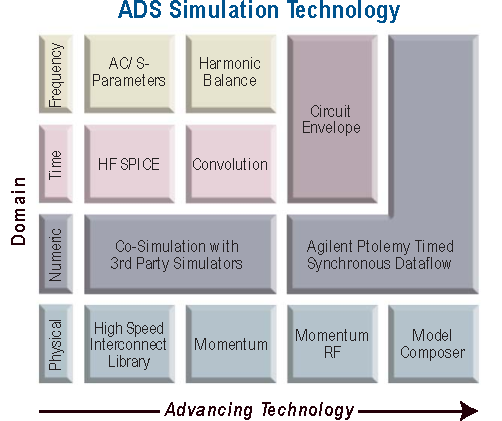
\includegraphics[width=12cm]{ADSSimTecno}
\caption{Simulatori RF che costituiscono l'ambiente ADS.}
\label{fig:ADSSimTecno}
\end{figure}

\par Nella figura \ref{fig:ADSSimTecno} sono rappresentate tutte le simulazioni in alta frequenza che il programma � in grado di effettuare ed i rispettivi domini in cui esse operano; la combinazione di esse permette appunto di caratterizzare e ottimizzare completamente il design del nostro sistema sotto opportune condizioni. In particolare, nel corso delle nostre esercitazioni abbiamo utilizzato solo alcuni di questi simulatori, il cui funzionamento dettagliato � rimandato al seguito quando saranno davvero sfruttate. Di seguito diamo solo alcuni cenni sui simulatori pi� importanti che costituiscono il \itt{design flow} di ADS.

\begin{figure}[ht!]
\centering
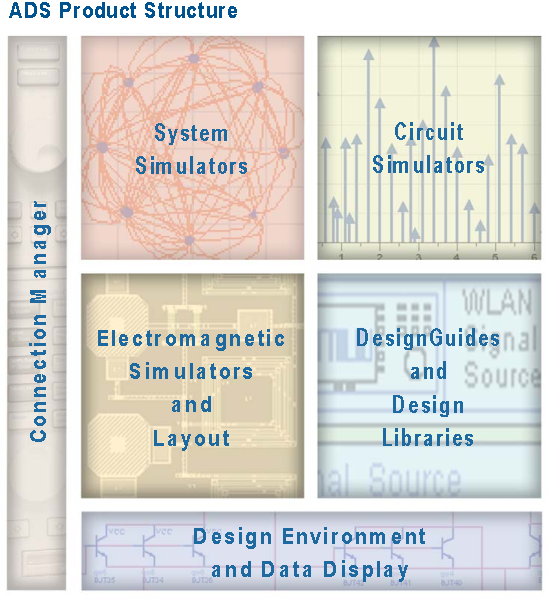
\includegraphics[width=10cm]{ADSProdStruct}
\caption{Interoperabilit� dei simulatori di ADS.}
\label{fig:ADSProdStruct}
\end{figure}

\par Per simulazioni a livello di sistema, l'\itt{Agilent Ptolemy Timed Synchronous Data Flow} \cite{Ptolemy} garantisce l'interoperabilit� tra i vari simulatori concordando i dati ottenuti ai vari livelli circuitali. Ptolemy permette quindi di analizzare le \itt{performances} di sistema ad esempio tramite \itt{bit error rate} e diagrammi delle costellazioni. Il simulatore \itt{Harmonic Balance} � stato invece introdotto per la prima volta dall' Agilent Technologies agli inizi degli anni ottanta ed � diventato il simulatore pi� importante nel dominio della frequenza per ottenere delle analisi rapide di circuiti non lineari, come verr� spiegato meglio in seguito. Oggi � in grado di gestire circuiti integrati ad alta densit� (VLSI) e pu� anche simulare divisori di frequenza digitali, sfruttando le capacit� del simulatore \itt{Transient} col \itt{Transient Assisted Harmonic Balance}. Il simulatore \itt{Circuit Envelope} invece � un'innovazione brevettata da Agilent che permette un'analisi accurata di un segnale modulato direttamente nel dominio della frequenza. Il simulatore \itt{RF System} realizza un'analisi di sistema ad alto livello, fornendo per ogni componente tutta una serie di parametri fondamentali quali cifra di rumore, IP3, 1 dBC, ecc. 
\par Un'accurata implementazione a livello fisico del circuito � di vitale importanza per predire le performance a livello hardware; per questo ADS include anche un ambiente di sviluppo fisico opportunamente congegnato per design di layout alle alte frequenze. Esso offre un elevato numero di capacit�, come la sincronizzazione del progetto con lo schematico; l'impiego di un motore per le interconnessioni fisiche ({real time}, che gira senza bisogno di dover lanciare nessuna utility secondaria) con \itt{Design Rule Checker} (DRC); la disponibilit� di simulatori elettromagnetici per circuiti planari come il \itt{Momentum} (2.5 D) completamente integrato con l'ambiente del layout. In questo modo aumenta per i progettisti la possibilit� di rilevare errori prima della produzione.
\par Un altro punto a favore della flessibilit� di questo software risulta essere la compatibilit� con molti altri design flow commerciali, ad esempio quelli basati su Cadence e Mentor, per citare alcuni dei pi� noti; in questo modo aumenta molto l'integrazione di quei prodotti che usano standard commerciali. 
\par Infine per quanto riguarda i problemi ad alta frequenza (riflessioni, {crosstalk}, ritardi di propagazione, integrit� del segnale, temporizzazioni, ecc.) ormai all'ordine del giorno nei circuiti che sfruttano clock ad altissima velocit�, ADS � in grado di modellarli e analizzarli con accuratezza grazie a librerie e ad opportuni strumenti di simulazione. In questo modo � possibile diminuire i problemi di interconnessioni ad alta frequenza prima della fabbricazione, riducendo quindi i costi e velocizzando il time to market.


%\par Il progetto di dispositivi di ricetrasmissione alle frequenze delle microonde richiede l'impiego di modelli accurati, che rispecchino il comportamento elettromagnetico dei componenti circuitali utilizzati e delle loro interconnessioni, le cui dimensioni diventano confrontabili con la lunghezza d'onda dei segnali informativi trattati.
%\par In alta frequenza, i componenti circuitali fisici presentano componenti parassiti non pi� trascurabili, e le loro impedenze possono fortemente discostarsi dal valore nominale atteso. Inoltre, i collegamenti tra i componenti diventano vere e proprie linee di trasmissione, per le quali � necessario conoscere l'impedenza caratteristica ai fini di un corretto convogliamento del segnale mediante gli opportuni adattamenti di impedenza alle estremit�.
%\par Vi � la necessit� di adattare, localmente, l'impedenza di uscita di un blocco a monte all'impedenza d'ingresso del blocco immediatamente a valle, in modo di massimizzare il trasferimento di potenza e minimizzare il coefficiente di riflessione. Qualsiasi perdita di segnale necessita di meccanismi di rigenerazione, operazioni che introducono rumore particolarmente degradante nella catena di ricezione.
%
%
%\par Le tecniche odierne di progettazione di circuiti in alta frequenza richiedono l'impiego di strumenti CAD\footnote{Computer Aided Design.} sofisticati che permettano di simulare il comportamento di tali circuiti.
%
%\DeclareFixedFootnote{\rep}{Text to repeat}
%
%
%


\pagestyle{headings}
\renewcommand\thefigure{\thechapter.\arabic{figure}}
\graphicspath{{img/lab1/}}
\chapter{Tecniche di adattamento}

%\section{Introduzione}

\par Nel seguente capitolo vengono introdotte le comuni tecniche di adattamento di impedenza (\itt{impedance matching}) impiegate nei circuiti a microonde, discutendone quindi le prestazioni in termini di banda di adattamento. L'obbiettivo dell'adattamento � quello di massimizzare il trasferimento di potenza da un blocco a monte a quello a valle, minimizzando l'onda riflessa alle discontinuit� di impedenza. Se, nell'intera banda del segnale, le perdite per riflessione sono sufficientemente trascurabili, viene massimizzato il rapporto segnale rumore a valle ed al contempo il segnale vi giunge privo di distorsioni. In figura \ref{fig:MatchingScheme} viene mostrato lo schema generico di adattamento di impedenza tra blocchi consecutivi.
\begin{figure}[ht!]
\centering % \hspace{2cm}
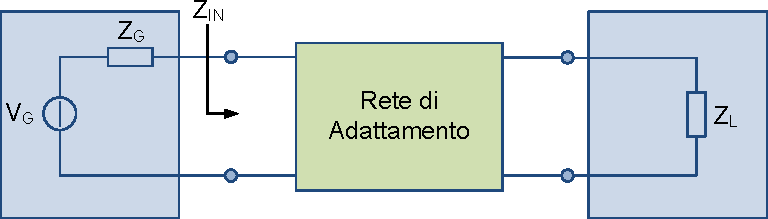
\includegraphics[width=12cm]{MatchingScheme}
\caption{Schema di adattamento.}
\label{fig:MatchingScheme}
\end{figure}In genere $\mathrm{Z}_\mathrm{G}$, impedenza del generatore a monte, e $\mathrm{Z}_\mathrm{L}$, impedenza del carico (\itt{load}) a valle sono specificate e bisogna sintetizzare la rete di adattamento. La realizzazione dell'adattamento � un caso particolare di trasformazione di impedenza: $\mathrm{Z}_\mathrm{IN}$, impedenza complessiva della cascata \textsf{rete di adattamento/carico}, deve coincidere con il complesso coniugato dell'impedenza $\mathrm{Z}_\mathrm{G}$ in modo che tutta la potenza disponibile dal generatore venga trasferita al carico (condizione di massimo trasferimento di potenza).

\par Le principali tecniche di adattamento d'impedenza utilizzate sono \cite{Rogers}: 
\begin{enumerate}
  \item la ``rete a L'', per la quale si impiegano opportuni componenti concentrati reattivi quali condensatori e induttori,
  \item gli ``stubs'', tronchi di linea di trasmissione terminati in corto circuito o circuito aperto che presentano idealmente, come i precedenti componenti della rete a L, impedenze puramente reattive di valore determinato dalla loro lunghezza e impedenza di linea che possone essere poste in parallelo o in serie sulla linea di trasmissione da adattare,
  \item il ``trasformatore a $\lambda / 4$'', tratto di linea ampio un quarto di lunghezza d'onda e con impedenza caratteristica tale da congiungere tratti di linea di impedenze diverse.
\end{enumerate} Queste tipologie di adattamenti presentano diversi comportamenti in termini di banda, determinando per ogni caso specifico una diversa larghezza spettrale a -10 dB.
\par Le prime esperienze sono state rivolte al problema dell'adattamento alla frequenza di 2 GHz di un carico di impedenza complessa $\mathrm{Z}_\mathrm{L} = 10 + j10 \ \Omega$ (carico ohmico-induttivo) ad un'impedenza $\mathrm{Z}_\mathrm{G} = 50 \ \Omega$, valore di riferimento nei circuiti RF. In effetti questo � il valore tipicamente scelto nei circuiti a microonde nella sintesi di linee di trasmissione e dispositivi passivi quali filtri, ibridi, divisori, ecc\footnote{I dispositivi attivi, per le loro impedenze d'ingresso e di uscita tipicamente complesse e dipendenti dalla polarizzazione, richiedono reti di adattamento a monte e a valle.}. Inizialmente si sono sfruttati componenti ideali privi di perdite, sia per gli adattamenti a costanti concentrate che distribuite. Successivamente sono stati utilizzati componenti reali, induttori e condensatori della \itt{Murata} per le reti a L e linee a microstriscia su substrati di vetronite per realizzare gli adattamenti con tratti di linea.

\subsubsection*{Simulatore \itt{S-Parameter}}

\par Per valutare $\mathrm{Z}_\mathrm{IN}$, e quindi dedurre il coefficiente di riflessione all'interfaccia corrispondente durante la sintesi della rete di adattamento, � stato utilizzato il simulatore lineare \itt{S-parameter} \cite{Sparams}. La simulazione S-parameter � un tipo di analisi AC ma per piccoli segnali, usata tipicamente per caratterizzare un componente passivo a RF o per stabilire le caratteristiche a piccolo segnale di un dispositivo attivo ad una specifica polarizzazione e temperatura. Se il circuito contiene elementi non lineari, il simulatore realizza prima una simulazione DC, quindi linearizza la loro caratteristica I-V intorno ai punti di polarizzazione, sfruttando per ogni dispositivo un modello lineare ben preciso. Il circuito lineare risultante viene analizzato come un dispositivo multi-porta, di cui si misurano i parametri di Scattering ($\mathrm{S}_\mathrm{ij}$ in generale, indicano il rapporto tra la porzione di onda riflessa alla porta i e quella incidente alla porta j), eccitando una porta per volta mentre le altre porte vengono chiuse su un carico adattato (su un'impedenza di riferimento, tipicamente 50 $\Omega$). Con questo accorgimento si ottiene la risposta del circuito attraverso i parametri S di tutte le porte, salvati poi in un \itt{dataset}. Trovati i parametri S, il simulatore permette anche di convertirli in parametri Z o Y, a seconda delle applicazioni di interesse. \`E possibile inoltre studiare il comportamento in frequenza di questi parametri, utili come nel nostro caso per realizzare un adattamento o studiare il comportamento di un filtro a microonde ad esempio. Inoltre questa analisi permette di simulare sia il ritardo di gruppo, utile per misurare la distorsione di fase negli amplificatori e nei filtri, che la cifra di rumore per un generico due porte. Nel caso di un circuito a N porte, la cifra di rumore viene misurata sempre su due porte stabilite dall'utente, mentre le altre vengono trattate come resistori per la simulazione del rumore.

\section{Matching ideale}

\par Il progetto di reti di adattamento � stato realizzato partendo dall'utilizzo di componenti di tipo ideale, questo, per poter poi osservare ed analizzare nel paragrafo \ref{sec:MR} i comportamenti di non idealit� introdotti dai componenti reali. Il carico da adattare � di tipo complesso con impedenza $\mathrm{Z}_\mathrm{L} = 10 + j10 \ \Omega$. Tramite l'ambiente di sviluppo ADS � stato realizzato e successivamente simulato un modello circuitale ideale che potesse adattare il carico in questione. Nel primo caso abbiamo utilizzato una rete a L, quindi una a singolo stub ed infine un trasformatore a $\lambda / 4$; questi passi sono ampiamente descritti di seguito.

\par Per analizzare l'adattamento del carico � stato creato un progetto inserendo in uno schematico il blocco dei parametri S e impostando la frequenza di lavoro a 2 GHz come illustrato nella seguente figura \ref{fig:ReteAdattADS}.
\begin{figure}[ht!]
\centering % \hspace{2cm}
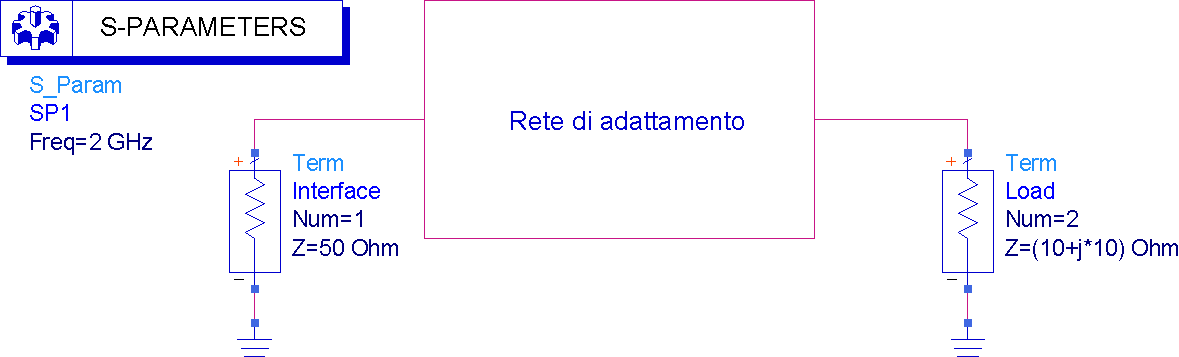
\includegraphics[width=12cm]{ReteAdattADS}
\caption{Rete di adattamento su ADS.}
\label{fig:ReteAdattADS}
\end{figure} I componenti \itt{Term} sono specifici dei parametri S e servono ad indicare al simulatore le interfacce alle quali si vogliono calcolare tali parametri.

\subsection{Rete a L}

\par L'adattamento � stato realizzato partendo da una rete ad L. Tali reti sono costituite da un condensatore C ed un induttore L messi uno in serie ed uno in parallelo al carico, formando cos� una sorta di L da cui la rete prende il nome. A seconda della disposizione di L e C si riesce ad adattare tutti i carichi passivi. Per analizzare la posizione del carico � stato utilizzato il circuito mostrato in figura \ref{fig:ReteAdattADS} cortocircuitando il blocco denominato ``rete di adattamento'', � stata quindi effettuata la simulazione e visualizzato il parametro $\mathrm{S}_\mathrm{11}$, S(1,1) in ADS, tramite carta di Smith (Vedi figura \ref{fig:RetiaL}).
\begin{figure}[ht!]
\centering % \hspace{2cm}
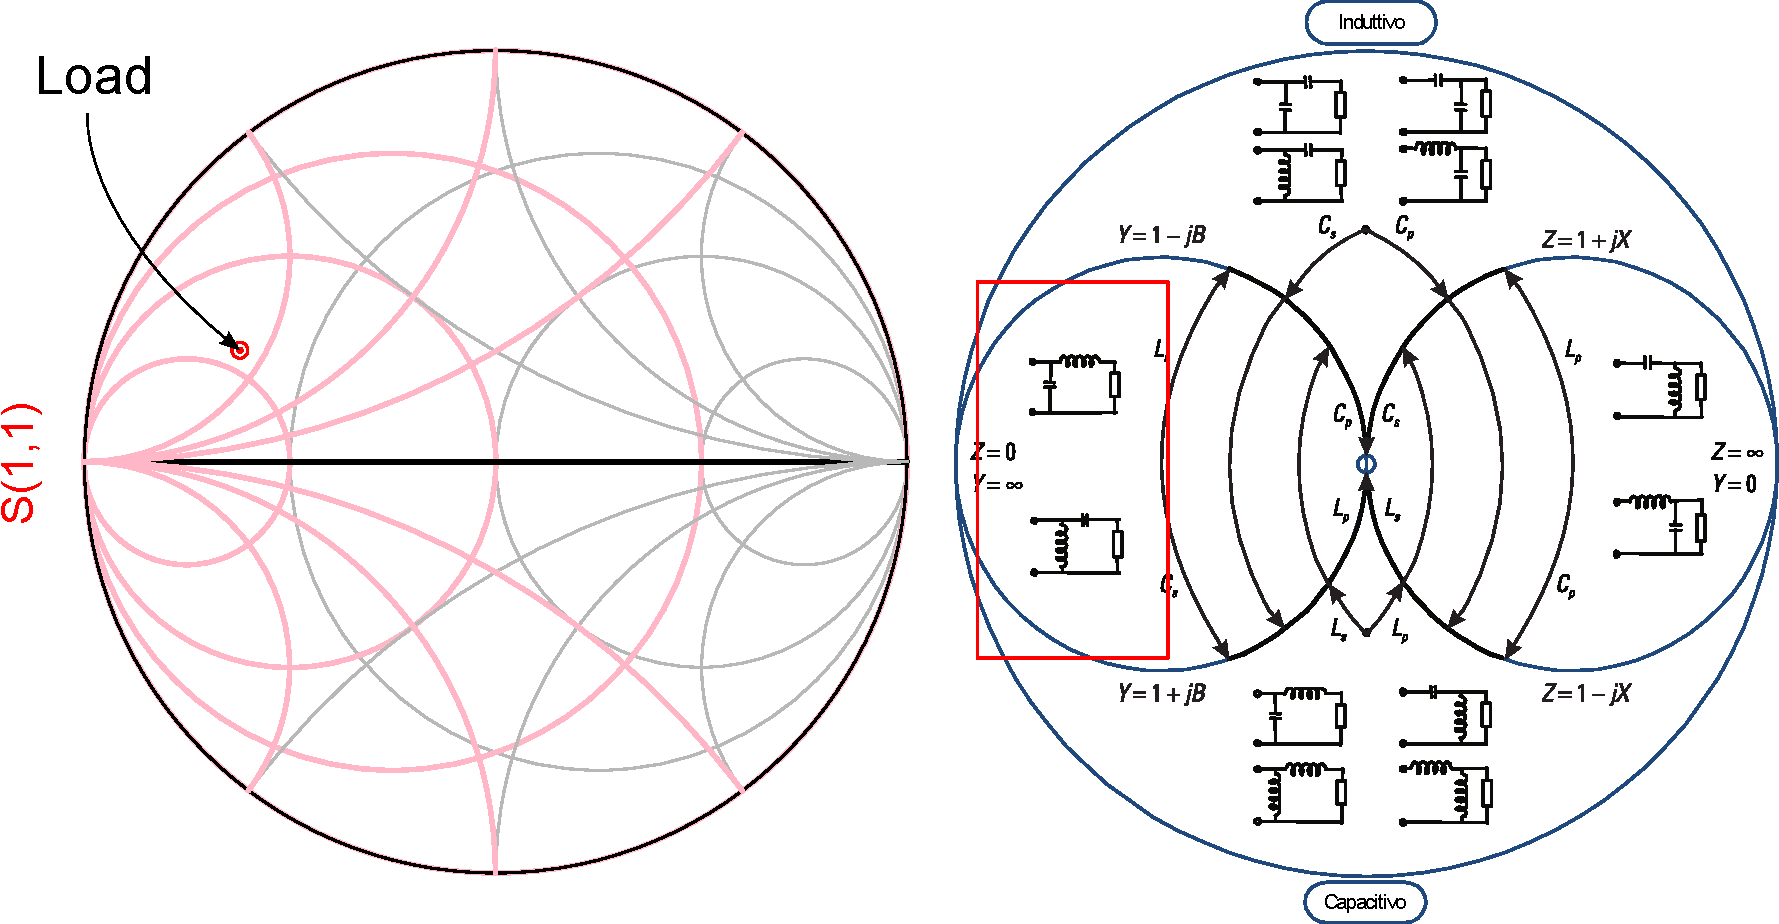
\includegraphics[width=15cm]{RetiaL}
\caption{Carico 10 + j10 $\Omega$ su carta di Smith e configurazioni di reti ad L possibili.}
\label{fig:RetiaL}
\end{figure} \`E stato quindi possibile decidere le configurazioni idonee dei componenti L e C, ovvero: 
\begin{enumerate}
\item Induttanza serie connessa a condensatore in parallelo , ``ISCP'',
\item Condensatore serie connesso ad induttanza parallelo, ``CSIP''.
\end{enumerate}

\subsubsection*{Induttanza serie e condensatore parallelo}

\par Per il punto ISCP � stata posizionata l'induttanza in serie al circuito, e tramite uno \itt{sweep} del valore induttivo abbiamo portato il carico  sul cerchio a conduttanza costante (evidenziato in blu in figura \ref{fig:SweepLschem}) passante per il centro della carta di Smith. Il valore di induttanza trovato � di 0,8 nH, tale cifra � stata quindi sostituita nel circuito.
\begin{figure}[ht!]
\centering % \hspace{2cm}
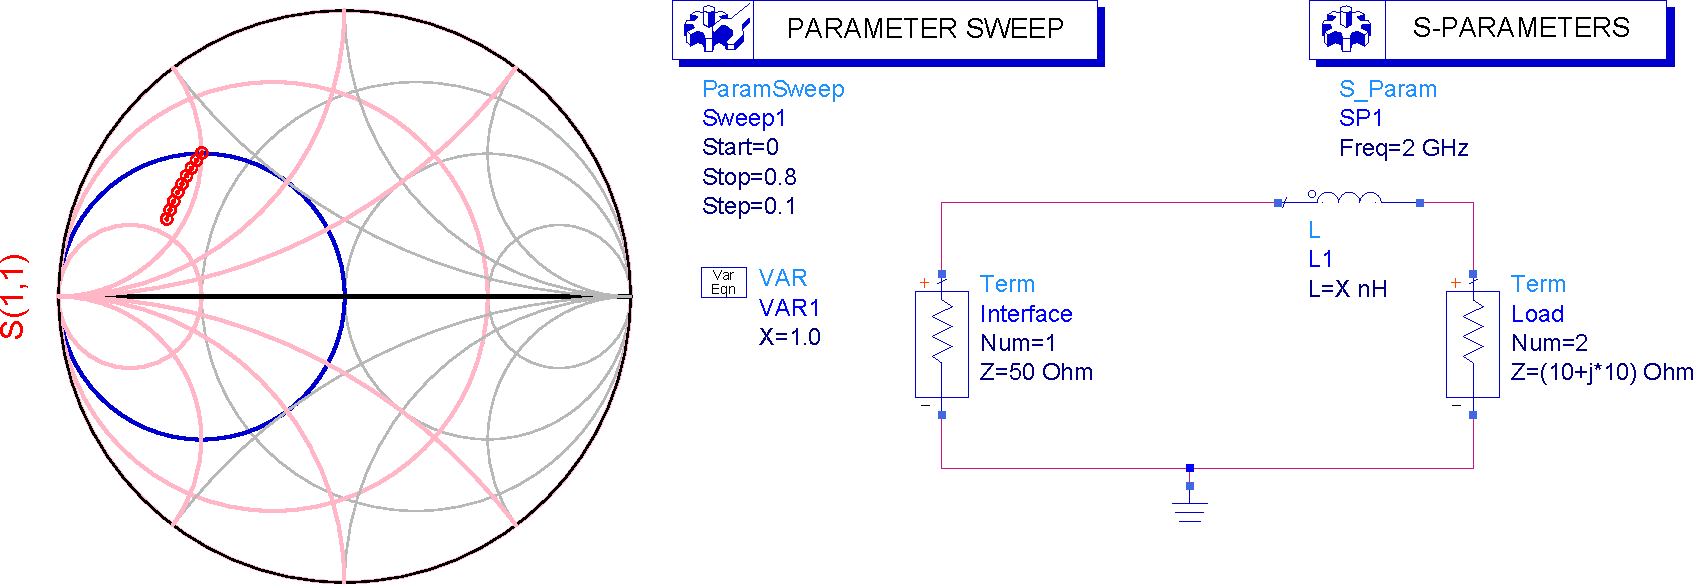
\includegraphics[width=15cm]{SweepLschem}
\caption{Sweep del valore dell'induttanza serie.}
\label{fig:SweepLschem}
\end{figure}

\par Dal risultato cos� ottenuto siamo quindi passati all'inserimento della capacit� parallelo che, determinando uno spostamento del carico lungo il cerchio a conduttanza costante, ha permesso l'adattamento perfetto. Il valore di capacit� trovato � di 3,183 pF (Vedi figura \ref{fig:SweepCschem}).

\begin{figure}[ht!]
\centering % \hspace{2cm}
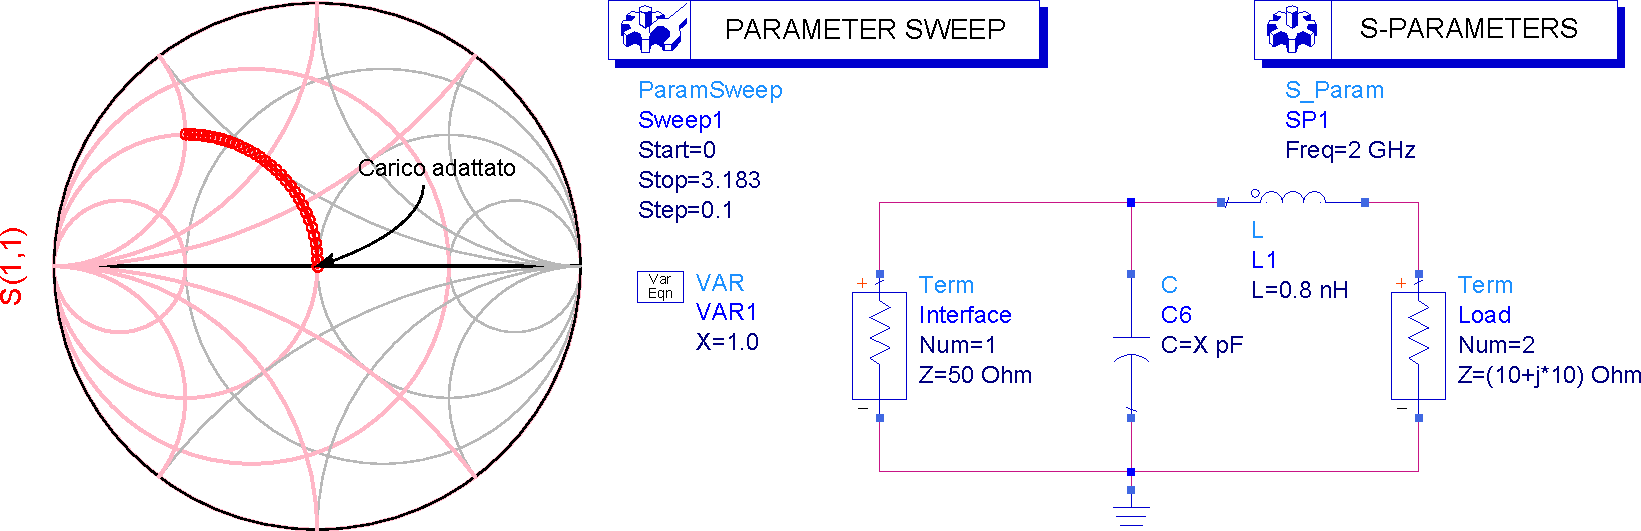
\includegraphics[width=15cm]{SweepCschem}
\caption{Sweep del valore della capacit� parallelo.}
\label{fig:SweepCschem}
\end{figure}

\par Per analizzare il comportamento in frequenza della rete di adattamento � stato quindi fatto uno sweep tra 1 GHz e 3 Ghz visualizzando il parametro di riflessione S(1,1). La banda per cui possiamo considerare un buon adattamento � quella per cui la riflessione non supera i -10 dB, valore per cui il 90\% della potenza giunge al carico, e nel nostro caso risulta essere di poco meno di 1 GHz (vedi fig. \ref{fig:BandLCschem}). Si pu� inoltre notare la bont� dell'adattamento alla frequenza desiderata (2 GHz) in quanto per tale valore vediamo corrispondere il minimo della nostra funzione.

\begin{figure}[ht!]
\centering % \hspace{2cm}
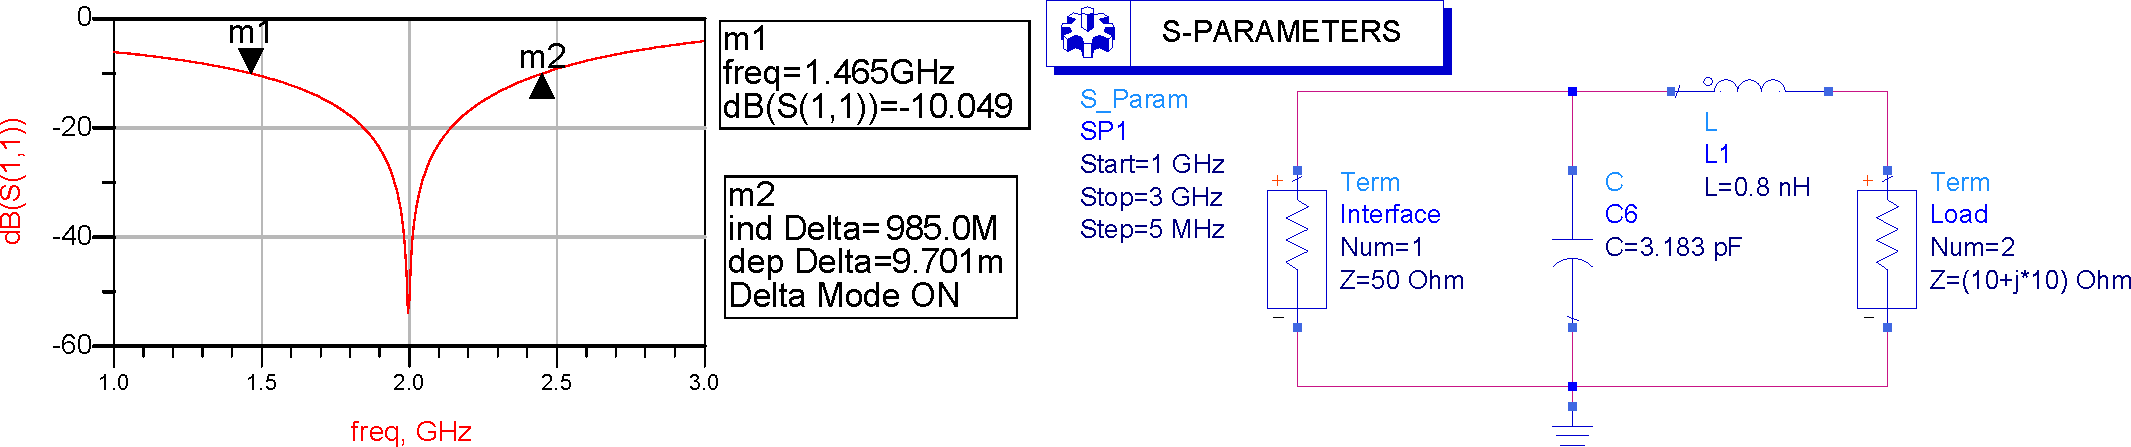
\includegraphics[width=16cm]{BandLCschem}
\caption{Banda adattamento ideale ad L ``ISCP''.}
\label{fig:BandLCschem}
\end{figure} 

\subsubsection*{Condensatore serie ed induttanza parallelo}

\par Passando al caso CSIP � stato seguito un procedimento analogo al precedente. Realizzato il circuito con il condensatore serie, tramite uno sweep � stato trovato il valore di C che portasse il carico sul cerchio ad conduttanza costante (dal punto Load al punto P1 in figura \ref{fig:CLSmith}), il valore risultante � di {2,652 pF}.
\begin{figure}[ht!]
\centering % \hspace{2cm}
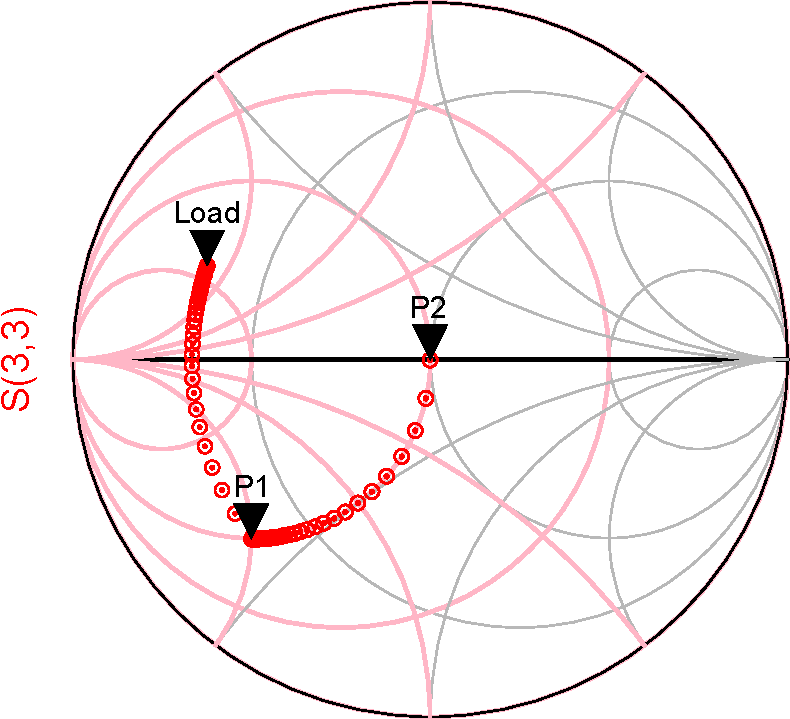
\includegraphics[width=6cm]{CLSmith}
\caption{Sweep di capacit� serie e induttanza parallelo.}
\label{fig:CLSmith}
\end{figure}  Dal punto P1 tramite l'induttore di valore L = {1,99 nH} posto in parallelo abbiamo ottenuto un adattamento perfetto in P2; anche questo dato � stato ottenuto tramite uno sweep di valori.

\par Una volta adattato il carico siamo passati a valutare la banda della rete, che risulta inferiore (Vedi in fig. \ref{fig:BandCLschem}) rispetto all'adattamento effettuato in precedenza. La banda � infatti di 627 MHz, circa i \nicefrac{2}{3} rispetto all'adattamento effettuato con induttore serie e capacit� parallelo.

\begin{figure}[ht!]
\centering % \hspace{2cm}
\includegraphics[width=16cm]{BandCLschem}
\caption{Banda adattamento ideale ad L ``CSIP''.}
\label{fig:BandCLschem}
\end{figure} 

\par Successivamente sono state utilizzate le reti di adattamento ISCP e CSIP per adattare sempre un carico di impedenza 10 + j10 $\Omega$ modellato per� non pi� da un componente Term, indipendente dalla frequenza, bens� dalla serie di una resistenza ed un'induttanza, quindi con impedenza dipendente dalla frequenza come illustrato in figura \ref{fig:FreqDep}. Sapendo che la resistenza introduce un carico puramente reale, e l'induttanza uno puramente immaginario, � bastato applicare le formule $\mathrm{Z}_\mathrm{R} = 10 \ \Omega$ e $\mathrm{Z}_\mathrm{L} = j\omega\mathrm{L} = j2{\pi}f\mathrm{L} = 10 \ \Omega$ per trovare i valori di R ed L appropriati. Il valore della resistenza � proprio di 10 $\Omega$, mentre il valore dell'induttanza � di {0.79 nH} tenuto conto della frequenza di lavoro di {2 GHz}. Realizzando un nuovo circuito con il nuovo carico abbiamo adattato prima con un condensatore parallelo connesso ad un'induttanza in serie. Inserendo l'induttanza, tramite uno sweep abbiamo trovato il valore che ha portato il carico sul cerchio a conduttanza costante, quindi, inserendo il condensatore abbiamo ottenuto perfetto adattamento. Successivamente � stata realizzata una rete di adattamento con un'induttanza parallelo connessa ad un condensatore serie. Con la medesima procedura, inserendo prima C e trovato il valore per portarci sul cerchio a conduttanza costante, inserendo quindi L, abbiamo ottenuto l'adattamento desiderato. I valori trovati delle induttanze e dei condensatori � identico a quello delle corrispondenti reti trovate in precedenza su carico indipendente dalla frequenza. Questo risultato � plausibile dato che l'impedenza complessa da adattare � la stessa, quindi, a parit� di componenti e della loro disposizione, le reti di adattamento non possono che risultare identiche.
\begin{figure}[ht!]
\centering % \hspace{2cm}
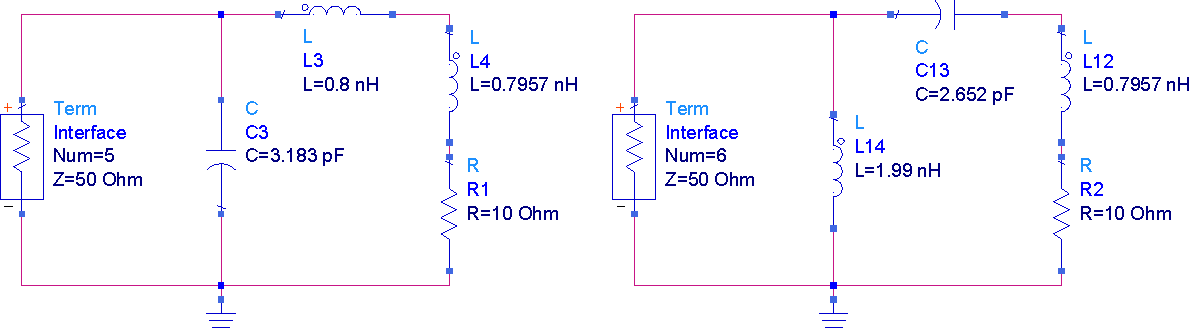
\includegraphics[width=12cm]{FreqDep}
\caption{Circuiti con carichi dipendenti dalla frequenza.}
\label{fig:FreqDep}
\end{figure}  Tramite uno sweep in frequenza del coefficiente di riflessione � stata quindi visualizzata la banda dei due nuovi casi modellati (Vedi figura \ref{fig:BandLCfinal}). Per mettere a confronto i risultati ottenuti � stato realizzato un grafico che mostrasse la risposta in frequenza delle quattro reti.
\begin{figure}[ht!]
\centering % \hspace{2cm}
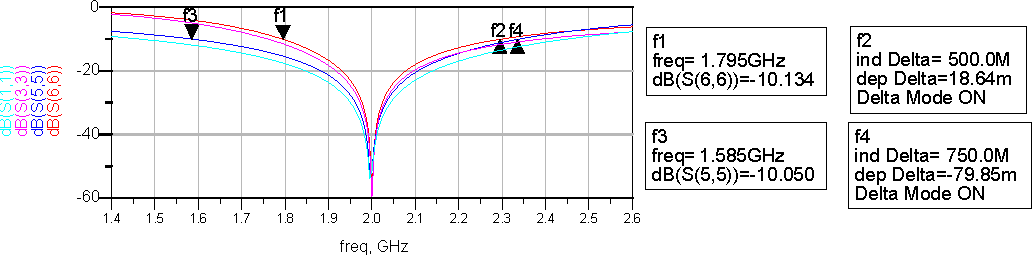
\includegraphics[width=16cm]{BandLCfinal}
\vspace{5mm}
\begin{tabular}{|ccccc|} \hline
Coefficiente di riflessione & Colore in figura & Tipologia di rete & Carico & Banda di adattamento \\ \hline
{S(1,1)} & ciano & ISCP & Term &  985 MHz \\
{S(3,3)} & {magenta} & {CSIP} &  {Term} &  {630 MHz} \\
{S(5,5)} & {blu} & {ISCP} &  {R-L} &  {750MHz} \\
{S(6,6)} & {rosso} & {CSIP} &  {R-L} &  {500MHz} \\ \hline
\end{tabular}
\caption{Confronto delle bande delle reti di adattamento.}
\label{fig:BandLCfinal}
\end{figure} 

Da quanto si pu� osservare in figura \ref{fig:BandLCfinal} ed apprezzare in termini numerici nella tabella sottostante, le bande dell'adattamento di carichi R-L sono pi� strette dei rispettivi casi con carichi di tipo term (985 MHz vs 750 MHz per il caso ISCP e 630 MHz vs 500 MHz per il caso CSIP). Questo effetto � dovuto al fatto che mentre il componente Term mantiene costante il suo valore di impedenza al variare della frequenza, la serie di R ed L invece no; il disadattamento ha quindi una crescita pi� rapida in quest'ultimo caso poich� si aggiunge il contributo di un carico ad impedenza variabile.

\subsection{Singolo Stub}

\par Utilizzando sempre un componente Term per modellare il carico di 10 + j10 $\Omega$ abbiamo preso in considerazione un adattamento ideale tramite stubs. La configurazione adottata per la rete di adattamento � quella di uno stub in circuito aperto in serie ad un tratto di linea di trasmissione. Lo stub � stato modellato tramite il componente TLOC (\itt{Transmission Line Open-Circuited Stub}) e la linea di trasmissione dal componente TLIN (\itt{Transmission Line}), entrambi componenti ideali e con impedenza caratteristica 50 $\Omega$.

\begin{figure}[ht!]
\centering % \hspace{2cm}
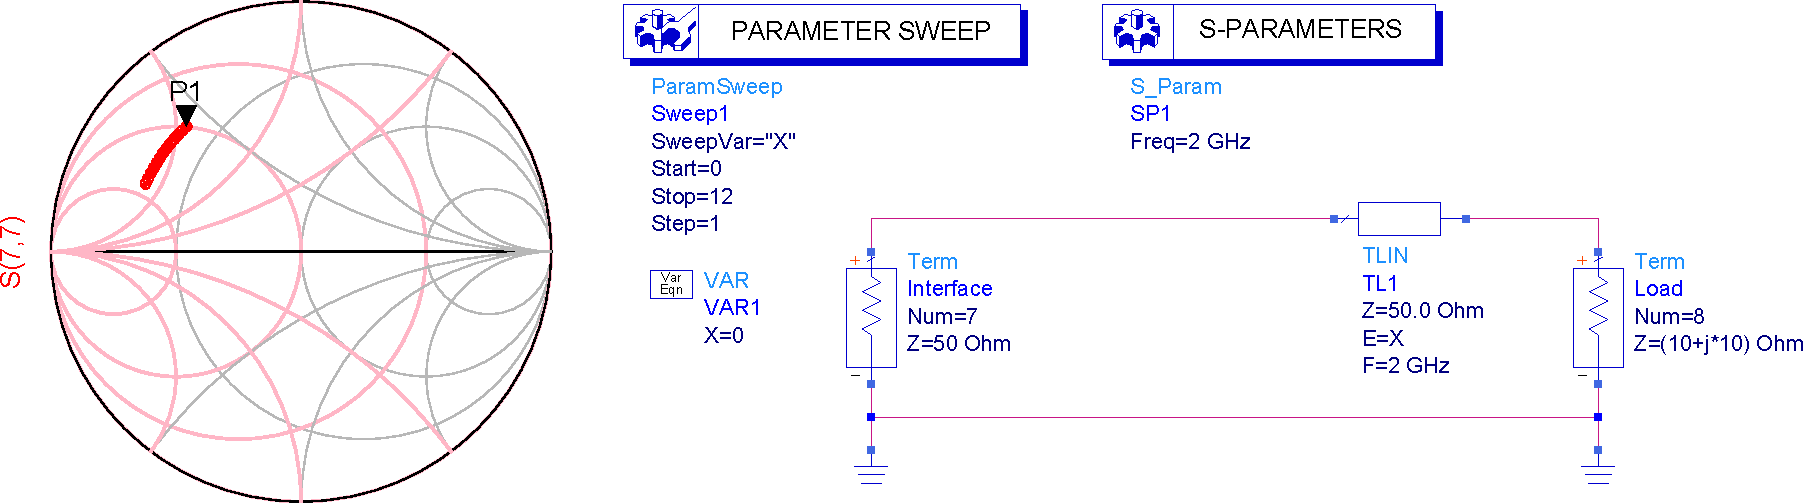
\includegraphics[width=16cm]{StubIdSchem1}
\caption{Sweep di lunghezza elettrica del componente TLIN.}
\label{fig:StubIdSchem1}
\end{figure} 

\par Partendo dall'inserimento di TLIN, � stato effettuato uno sweep di lunghezza elettrica che ha portato il carico sul cerchio a conduttanza costante (figura \ref{fig:StubIdSchem1}), il valore della lunghezza cos� trovata � di 12 gradi elettrici. Fatto ci�, � stato inserito lo stub in cortocircuito TLOC, anche qui con uno sweep della lunghezza elettrica abbiamo portato il carico al centro della carta di Smith (figura \ref{fig:StubIdSchem2}).

\begin{figure}[ht!]
\centering % \hspace{2cm}
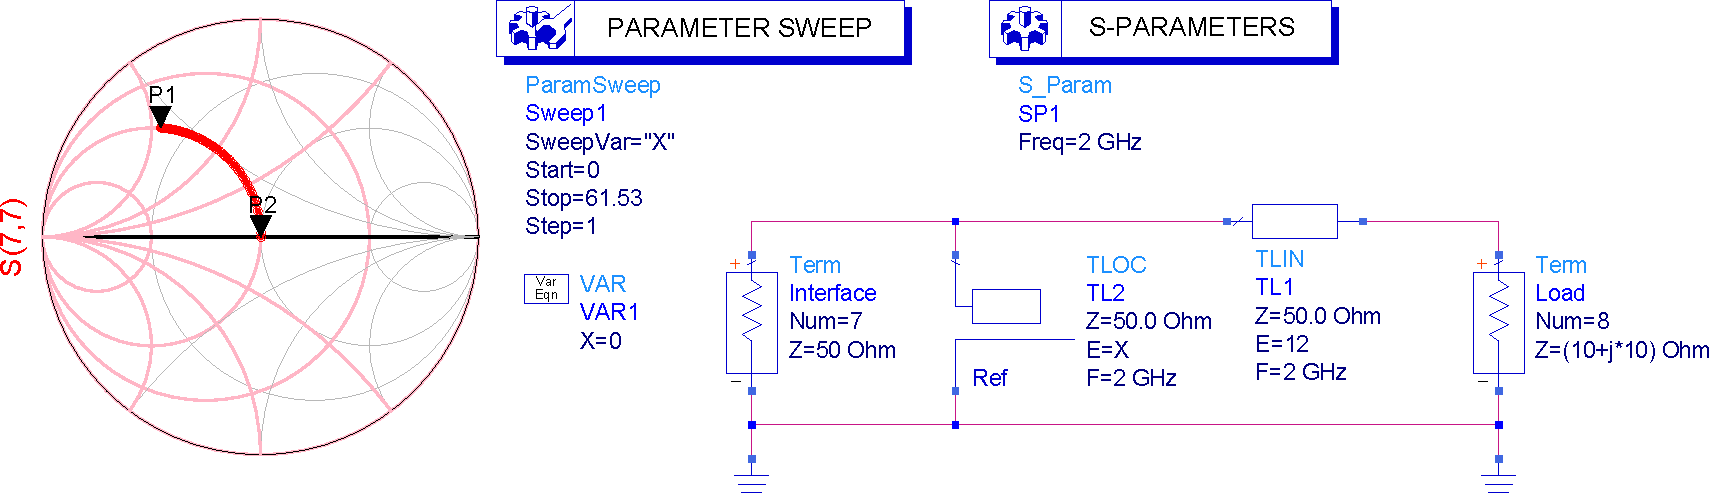
\includegraphics[width=16cm]{StubIdSchem2}
\caption{Sweep di lunghezza elettrica del componente TLOC.}
\label{fig:StubIdSchem2}
\end{figure} 
 
Impostando al componente TLOC la lunghezza di 61,53 gradi elettrici ottenuta dalla simulazione, � stato effettuato uno sweep in frequenza per osservare la banda della rete di adattamento. Da come si pu� osservare in figura \ref{fig:StubIdSchem} essa risulta essere di 510 MHz sempre considerando -10 dB come soglia di buon adattamento.

\begin{figure}[ht!]
\centering % \hspace{2cm}
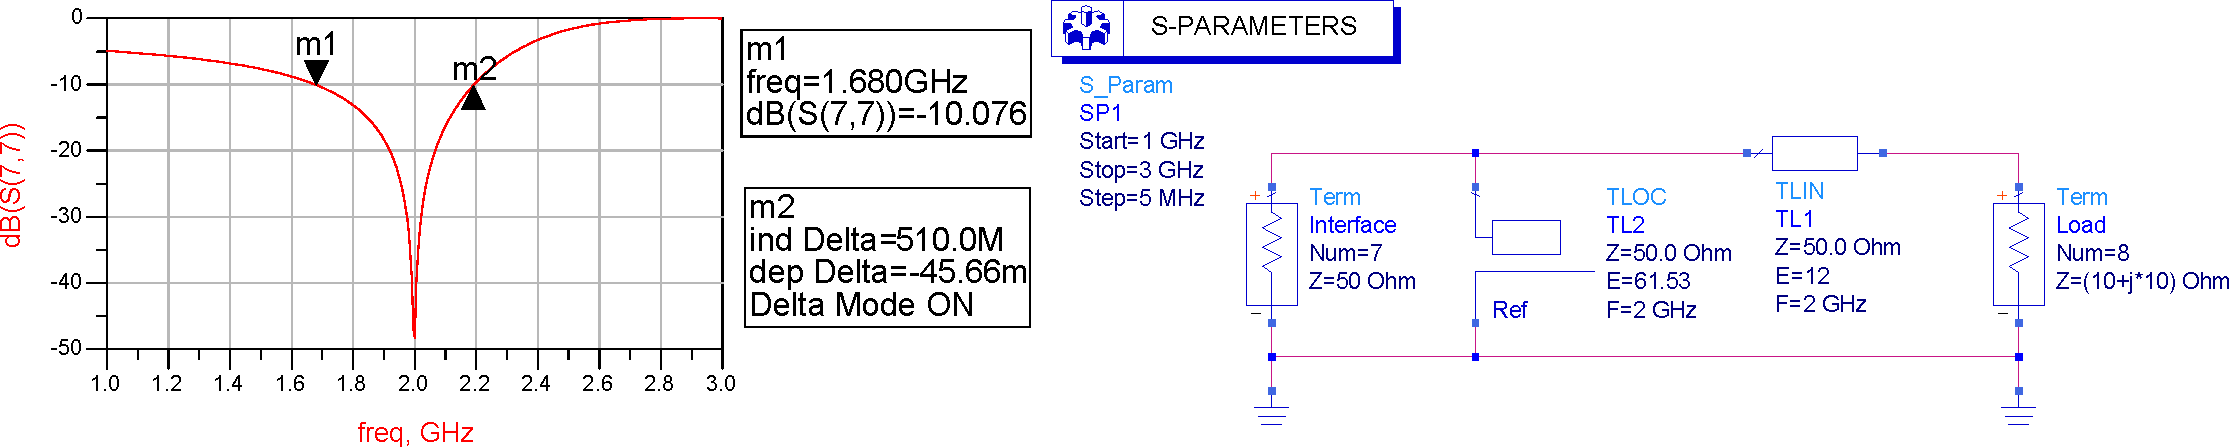
\includegraphics[width=16cm]{StubIdSchem}
\caption{Banda della rete di adattamento con stub ideale.}
\label{fig:StubIdSchem}
\end{figure}

\subsection{\texorpdfstring{ Trasformatore a $\lambda / 4$}{ Trasformatore a Lambda Quarti}} \label{sec:Lambda4th}% $\lambda / 4$}

\par Per l'adattamento con trasformatore a $\lambda / 4$ ideale, � stata realizzata una rete di adattamento composta dalla serie di due componenti TLIN impostati sulla frequenza di lavoro di 2 GHz. Il primo elemento, TL3, � stato inserito in serie alla rete e, tramite uno sweep della sua lunghezza elettrica, ha permesso di annullare la parte induttiva del carico portandolo quindi sulla retta ad impedenza reale (figura \ref{fig:Lambda4th1Schem}), nel punto P1 per il quale $\mathrm{Z}_\mathrm{IN} = 260,42 \ \Omega$.

\begin{figure}[ht!]
\centering % \hspace{2cm}
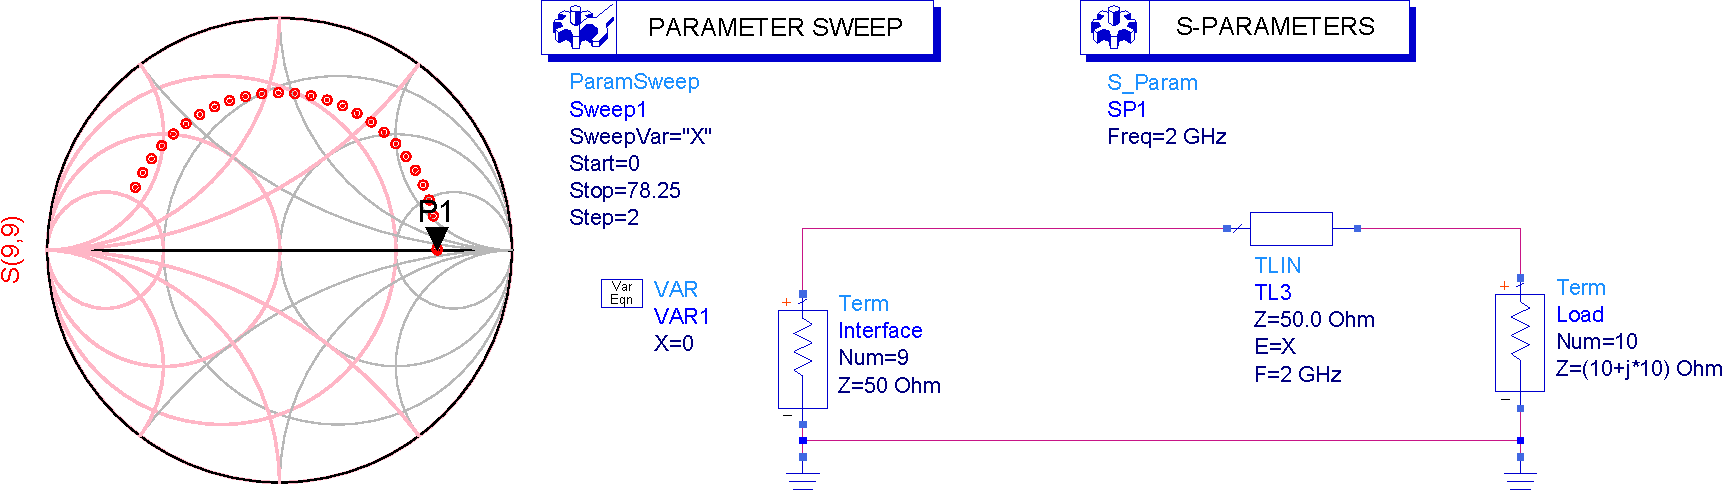
\includegraphics[width=16cm]{Lambda4th1Schem}
\caption{Sweep della lunghezza elettrica di TL3.}
\label{fig:Lambda4th1Schem}
\end{figure}

La lunghezza trovata di 78,25 gradi elettrici � stata impostata come parametro del componente TL3, quindi, abbiamo proceduto con l'inserimento serie del secondo componente TLIN ovvero TL4. Quest'ultimo, dovendo svolgere la funzione di trasformatore a $\lambda / 4$ � stato settato con lunghezza di 90 gradi elettrici. Il trasformatore a $\lambda / 4$ permette, al variare della sua impedenza caratteristica, di muovere il carico lungo l'asse ad impedenza reale. Tramite lo sweep dell'impedenza di TL4 � stato possibile trovare il valore $\mathrm{Z}_\mathrm{\lambda / 4}$ = 114,11 $\Omega$, tramite cui il carico risulta perfettamente adattato (figura \ref{fig:Lambda4th2Schem}). Il valore di $\mathrm{Z}_\mathrm{\lambda / 4}$ poteva essere calcolato mediante la relazione $\mathrm{Z}_\mathrm{\lambda / 4} = \sqrt{\mathrm{Z}_\mathrm{IN} \cdot \mathrm{Z}_\mathrm{OUT}} = \sqrt{ 50 \cdot 260,42 } \ \Omega$.

\begin{figure}[ht!]
\centering % \hspace{2cm}
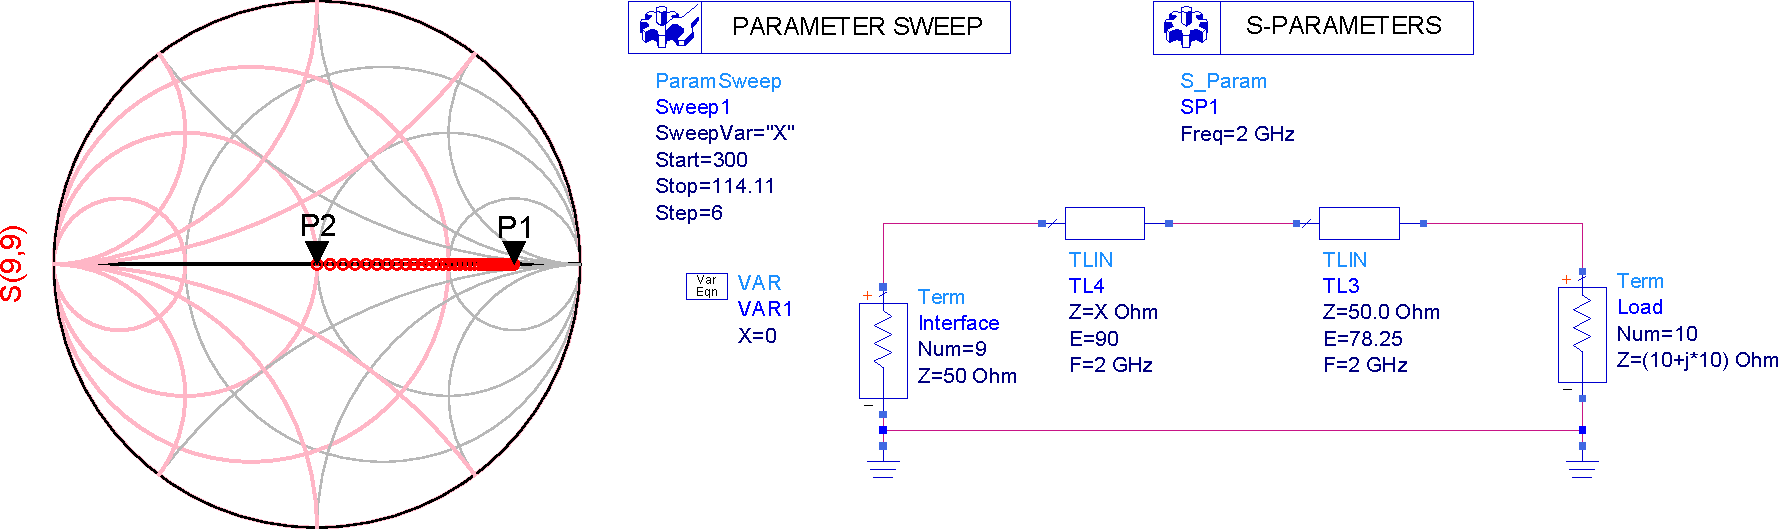
\includegraphics[width=16cm]{Lambda4th2Schem}
\caption{Sweep dell'impedenza di TL4.}
\label{fig:Lambda4th2Schem}
\end{figure}

Il passo successivo � stato quello di valutare la banda della rete di adattamento mostrata in figura \ref{fig:Lambda4th1Band}. Come nei casi precedentemente illustrati questa operazione � stata effettuata tramite la visualizzazione del coefficiente di riflessione facendo variare la frequenza con una funzione di sweep.
Da come si pu� verificare confrontando con i risultati precedentemente ottenuti (figure \ref{fig:BandLCfinal} e \ref{fig:StubIdSchem}) la banda di questa tipologia di rete � molto stretta.

\begin{figure}[ht!]
\centering % \hspace{2cm}
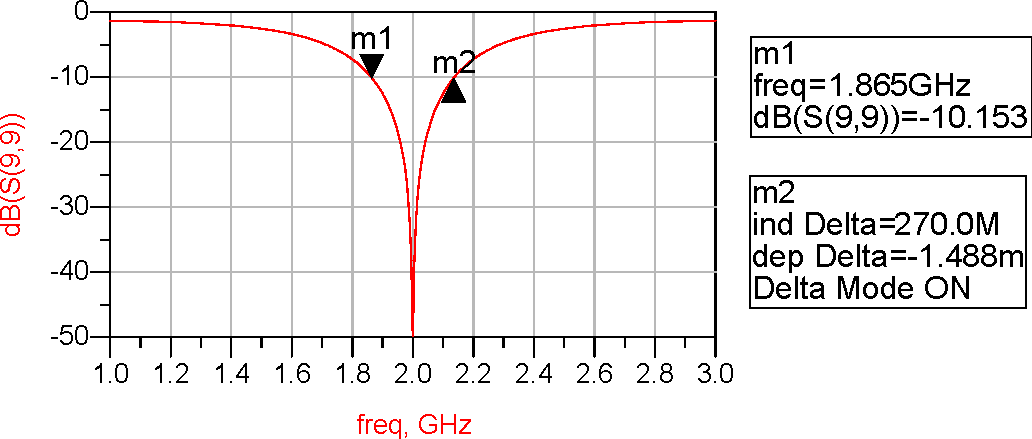
\includegraphics[width=12cm]{Lambda4th1Band}
\caption{Banda della rete di adattamento a $\lambda / 4$.}
\label{fig:Lambda4th1Band}
\end{figure}

%\newpage
\section{Matching reale} \label{sec:MR}

\par Successivamente all'analisi di reti di adattamento ideali siamo passati all'utilizzo di componenti reali utilizzando la libreria della Murata, produttore leader di dispositivi passivi realizzati su base ceramica \cite{Murat}, che comprende induttori e condensatori ad alte prestazioni (alte frequenze di risonanza). Le caratteristiche dell'analisi sono rimaste invariate per poter confrontare meglio i risultati finora ottenuti con quelli che procederemo qui di seguito ad ottenere. Quindi anche nelle prossime simulazioni verranno adattati carichi complessi di tipo induttivo del valore di 10 + j10 $\Omega$, e la frequenza di lavoro sar� di 2 GHz.

\subsection{Rete a L}

\par L'adattamento tramite rete a L con componenti Murata � stata suddivisa anche in questo caso in due parti: ISCP e CSIP.

\subsubsection*{Induttanza serie e condensatore parallelo} \label{sec:LCMurata}

\par Per il caso ISCP � stato preso come riferimento il modello circuitale dell'analogo caso ideale (Vedi fig. \ref{fig:BandLCschem}). L'induttanza serie trovata era di {0,8 nH}, � stata quindi modellata con il componente LQP03, del valore di esattamente {0,8 nH}. Anche il condensatore di valore {3,183 pF} � stato modellato con il componente GJM03 del valore di {3,2 pF} (Vedi fig. \ref{fig:LCMurata1}). 

\begin{figure}[ht!]
\centering % \hspace{2cm}
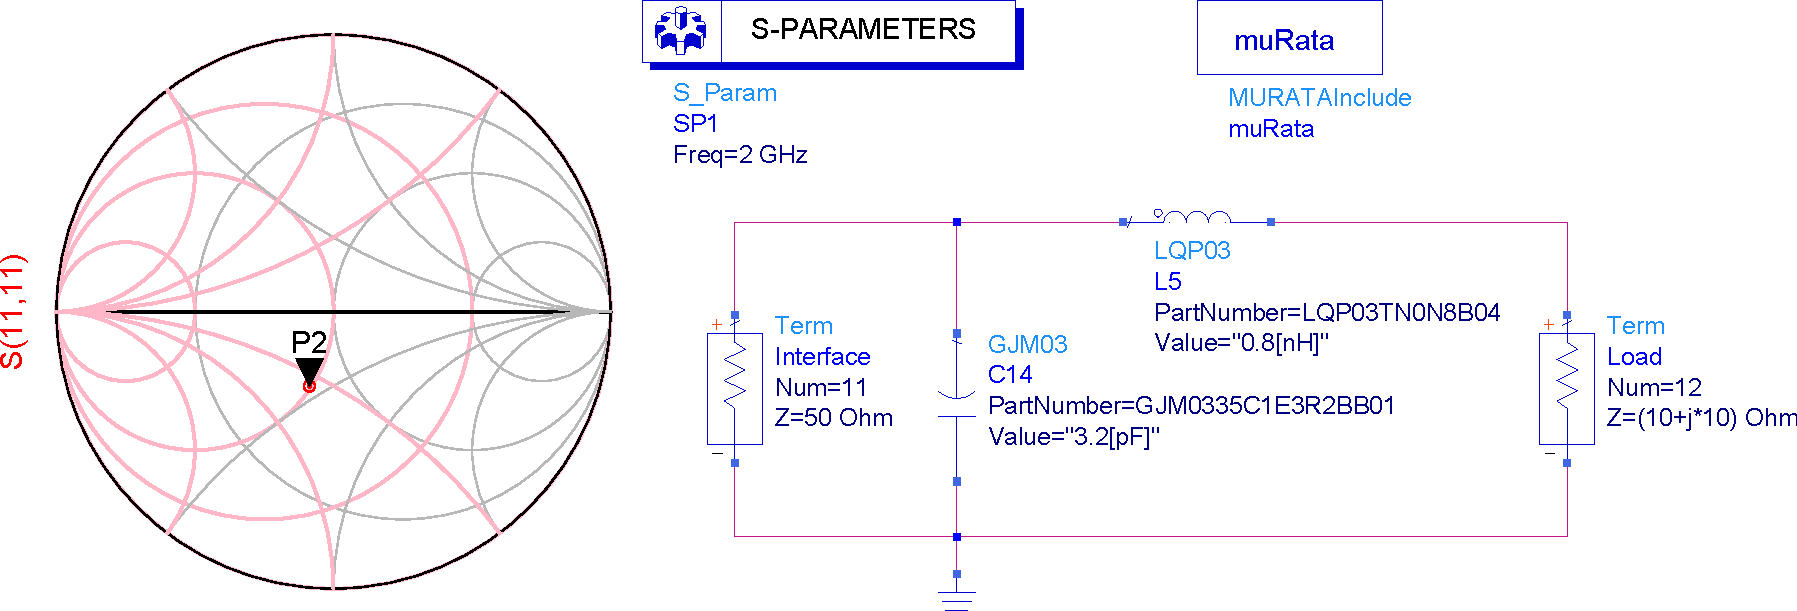
\includegraphics[width=16cm]{LCMurata1}
\caption{Rete a L con componenti Murata.}
\label{fig:LCMurata1}
\end{figure}
 
\par La scelta dei componenti � stata effettuata osservando che rispettassero i requisiti di frequenza necessari, ampiamente superati sia da L la cui banda � di {10 MHz - 6 GHz} che da C con banda {300 kHz - 20 GHz}. Dopo aver effettuato la simulazione, abbiamo osservato tramite carta di Smith che, pur essendo entrambi i componenti con valore nominale molto vicino se non addirittura identico a quello desiderato, il carico non � pi� perfettamente adattato. Questo fenomeno � dovuto al fatto che i componenti reali sono affetti da componenti parassiti, e ci� si ripercuote sul coefficiente di riflessione della rete di adattamento. Per poter ovviare a questo fenomeno � stato ricercato un modello di rete di adattamento reale pi� efficiente, impiegando dei componenti reali Murata di valore diverso ma prossimo a quello ideale. Studiando l'andamento del carico al variare dei componenti L e C � stata prevista e quindi verificata la migliore configurazione. Questa � modellata sempre dai componenti LQP03 e GJM03 visti in precedenza, ma con valori di induttanza e capacit� diversi, rispettivamente 0,6 nH e 2,7 pF (Vedi fig. \ref{fig:LCMurata2}).

\begin{figure}[ht!]
\centering % \hspace{2cm}
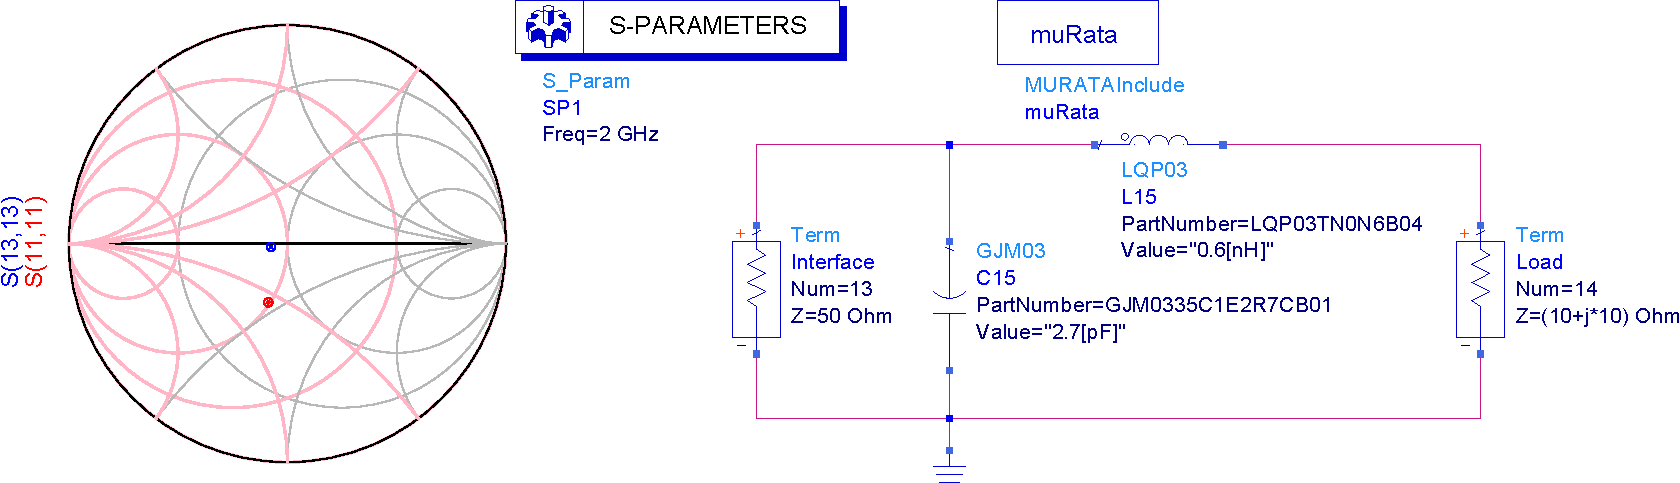
\includegraphics[width=16cm]{LCMurata2}
\caption{Rete ad L reale ottimizzata.}
\label{fig:LCMurata2}
\end{figure} 

\par Il parametro S(13,13) visibile nell'immagine \ref{fig:LCMurata2} � il coefficiente di riflessione del circuito ottimizzato, quest'ultimo � nettamente pi� vicino al centro della carta di Smith rispetto al precedente, realizzando dunque un miglior adattamento per la frequenza di 2 GHz. Questo per� non implica necessariamente una situazione migliore poich� talvolta un miglior adattamento alla frequenza di lavoro comporta un restringimento della banda della rete. Il passo successivo � stato quindi quello di verificare le risposte in frequenza di entrambi i circuiti analizzati.

\begin{figure}[ht!]
\centering % \hspace{2cm}
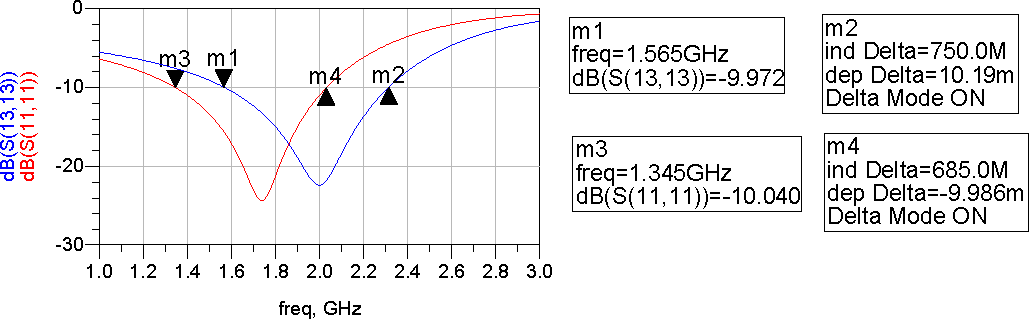
\includegraphics[width=12cm]{LCMurataBand}
\caption{Confronto delle risposte in frequenza.}
\label{fig:LCMurataBand}
\end{figure} 

Da come si pu� osservare in figura \ref{fig:LCMurataBand} in questo caso la soluzione trovata � veramente ottima, poich� oltre ad un migliore adattamento a 2 GHz abbiamo anche un incremento della banda che passa da {685 MHz} del caso precedente a {750 MHz} di quello attuale. La rete ottimizzata quindi, � la migliore sotto entrambi i punti di vista.

\subsubsection*{Condensatore serie e induttanza parallelo}

\par Per il caso CSIP � stato preso come riferimento il modello circuitale dell'analogo caso ideale (Vedi fig. \ref{fig:BandCLschem}). Anche in questo caso abbiamo realizzato un circuito sostituendo i componenti ideali con i rispettivi reali della libreria Murata. Il condensatore in serie al carico, di valore {2,652 pF} � stato modellato con il componente GJM03 del valore di {2,7 pF}. L'induttanza in parallelo trovata era di {1,99 nH}, � stata quindi modellata con il componente LQP03, del valore di {2 nH} (Vedi fig. \ref{fig:CLMurata1}). I componenti Murata utilizzati sono fondamentalmente gli stessi del punto \ref{sec:LCMurata} a differenza di qualche piccolo parametro ininfluente ai fini della nostra analisi.

\begin{figure}[ht!]
\centering % \hspace{2cm}
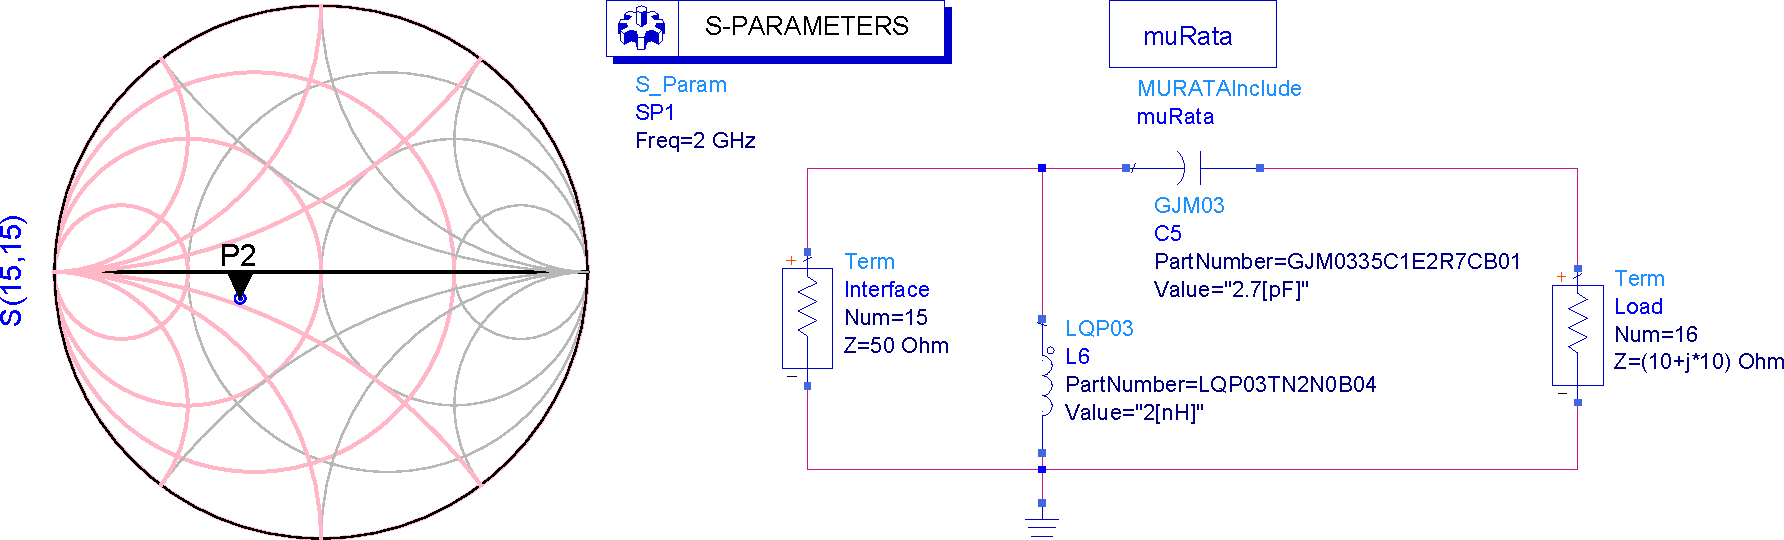
\includegraphics[width=16cm]{CLMurata1}
\caption{Rete ad L con componenti Murata.}
\label{fig:CLMurata1}
\end{figure} 

Anche in questo caso la posizione del carico sulla carta di Smith � ben lontano dal caso ideale, siamo quindi intervenuti per ottimizzare anche questa rete in modo da compensare le perdite dovute ai componenti reali. Dopo alcune prove, la soluzione ottimale � stata individuata utilizzando un condensatore del valore di {2,2 pF} e lasciando immutata l'induttanza ai suoi {2 nH}. Il circuito ottenuto, mostrato in figura \ref{fig:CLMurata2} fa notare come questa configurazione sia molto vicina a quella ideale.

\begin{figure}[ht!]
\centering % \hspace{2cm}
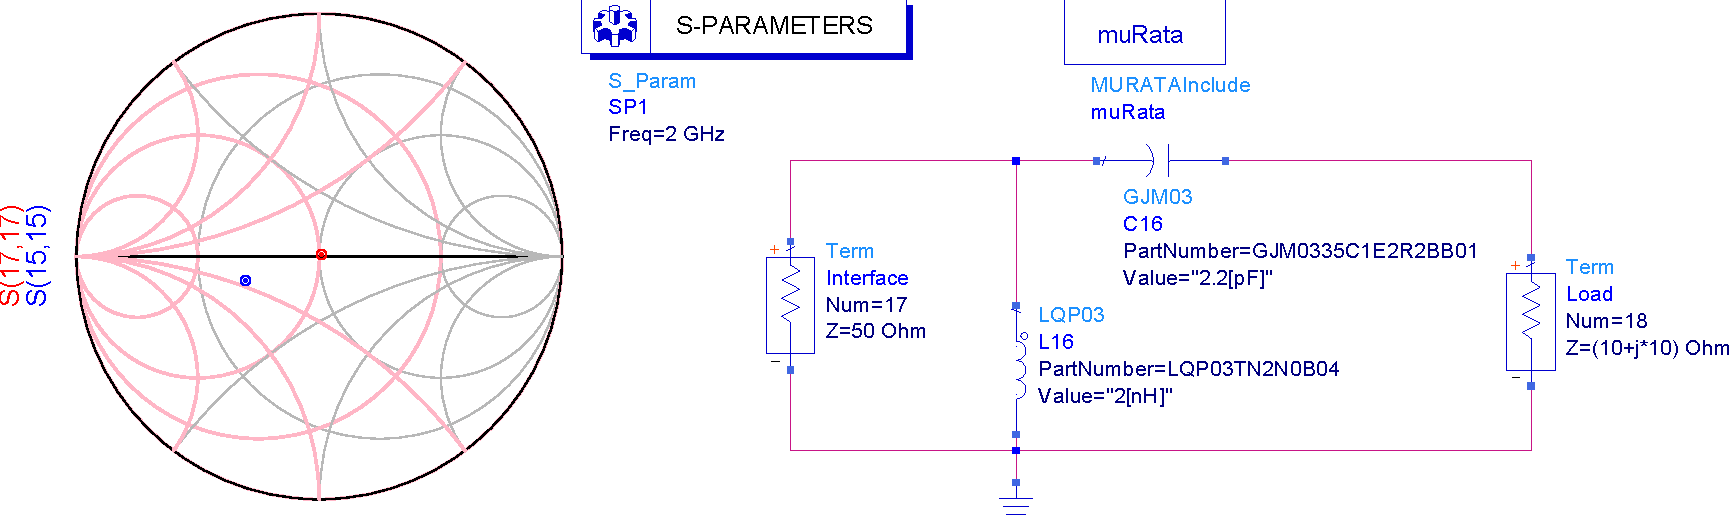
\includegraphics[width=16cm]{CLMurata2}
\caption{Rete ad L reale ottimizzata.}
\label{fig:CLMurata2}
\end{figure}

Tramite uno sweep della frequenza nel range {1 Ghz - 3 GHz} � stato possibile verificare le prestazioni del modello ottimizzato che presenta una attenuazione della riflessione a {2 GHz} (la nostra frequenza di lavoro) superiore ai {50 dB}. 

\begin{figure}[ht!]
\centering % \hspace{2cm}
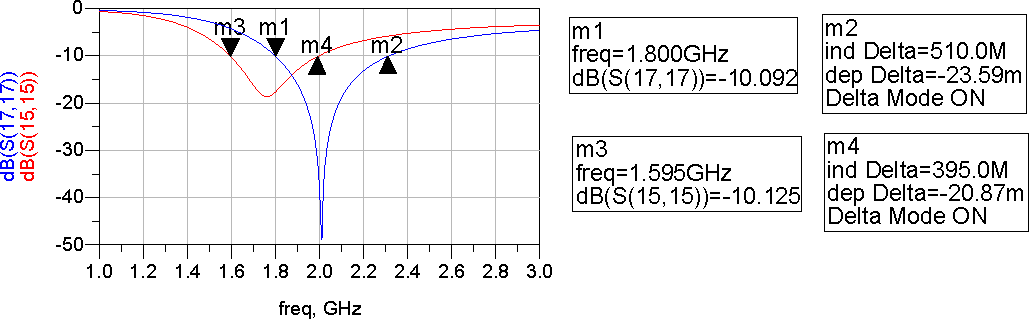
\includegraphics[width=12cm]{CLMurataBand}
\caption{Confronto delle risposte in frequenza.}
\label{fig:CLMurataBand}
\end{figure}

La banda del circuito ottimizzato � inoltre centrata quasi perfettamente alla frequenza di nostro interesse.

\subsection{Singolo Stub}

\par Per l'adattamento del carico con singolo stub, sono stati utilizzati i modelli di linee di trasmissione in microstriscia riferiti ad un substrato ``MSub''. I componenti utilizzati sono: MLIN, modello di un tratto di linea in microstriscia, ed MLEF, tratto di linea in microstriscia in circuito aperto che tiene conto anche dell'\itt{end effect}, ovvero dello sfrangiamento del campo elettrico in prossimit� della discontinuit� del circuito aperto. � stato inoltre utilizzato il componente MTEE per modellare anche la discontinuit� che si trova all'interfaccia dell'inserimento tra MLIN ed MLEF. Il substrato di riferimento, modellato dal componente MSUB presenta uno spessore h di 1600 $\mu$m, la costante dielettrica relativa $\epsilon_\mathrm{r}$ � di $4,36$, la permeabilit� relativa $\mu_\mathrm{r}$ � pari a 1, la conducibilit� $\sigma$ � di $5,957 \cdot 10^{7} \ S/m$, lo spessore del conduttore \itt{t} � di 32 $\mu$m, la tangente di perdita $\tan(\delta)$ � 0,0177 e la rugosit� superficiale del conduttore (\itt{Rough}) � di 1 $\mu$m (Vedi fig. \ref{fig:LineCalcStub}).

\begin{figure}[ht!]
\centering % \hspace{2cm}
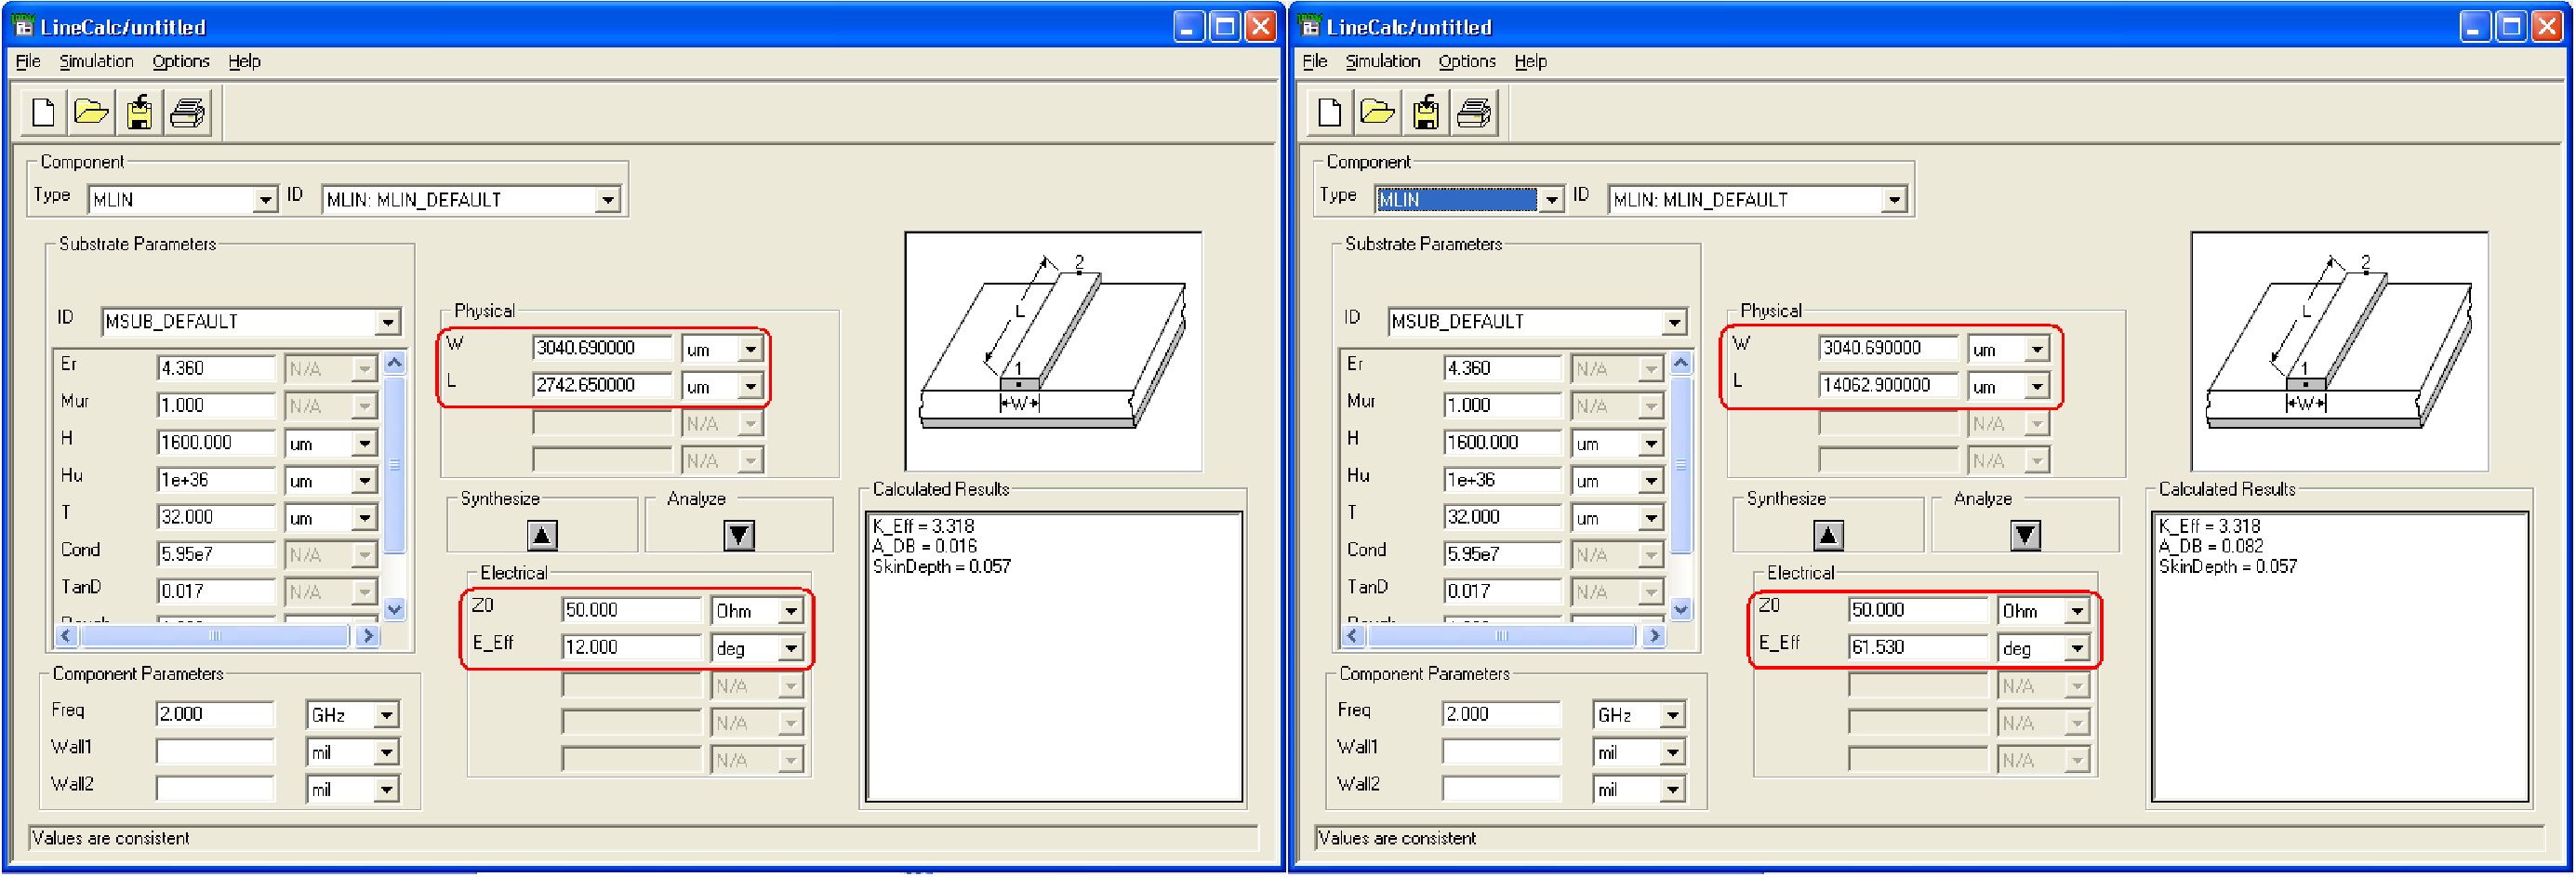
\includegraphics[width=16cm]{LineCalcStub}
\caption{Utilizzo del tool LineCalc per trovare i parametri fisici.}
\label{fig:LineCalcStub}
\end{figure}

Anche in questo caso come nel precedente, il componente in serie MLIN porta il carico sul cerchio a conduttanza costante; da quel punto poi, il tratto di linea in parallelo MLEF effettua l'adattamento. Per trovare i valori rispettivamente di MLIN ed MLEF abbiamo utilizzato il tool {LineCalc} (Vedi fig. \ref{fig:LineCalcStub}) che, dopo aver impostato i parametri del substrato, ci ha permesso di passare dai parametri elettrici della linea a quelli fisici. I parametri elettrici sono quelli trovati nel caso ideale. Il tratto di linea in serie aveva lunghezza elettrica di 12 gradi ed un'impedenza di 50 $\Omega$ e il tool ci ha quindi fornito la larghezza W = 3041 $\mu$m e la lunghezza L = 2743 $\mu$m della MLIN. Il tratto di linea in parallelo aveva invece una lunghezza di 61.53 gradi elettrici, che sono diventati 14063 $\mu$m di lunghezza (Vedi fig. \ref{fig:StubRe1}).

\begin{figure}[ht!]
\centering % \hspace{2cm}
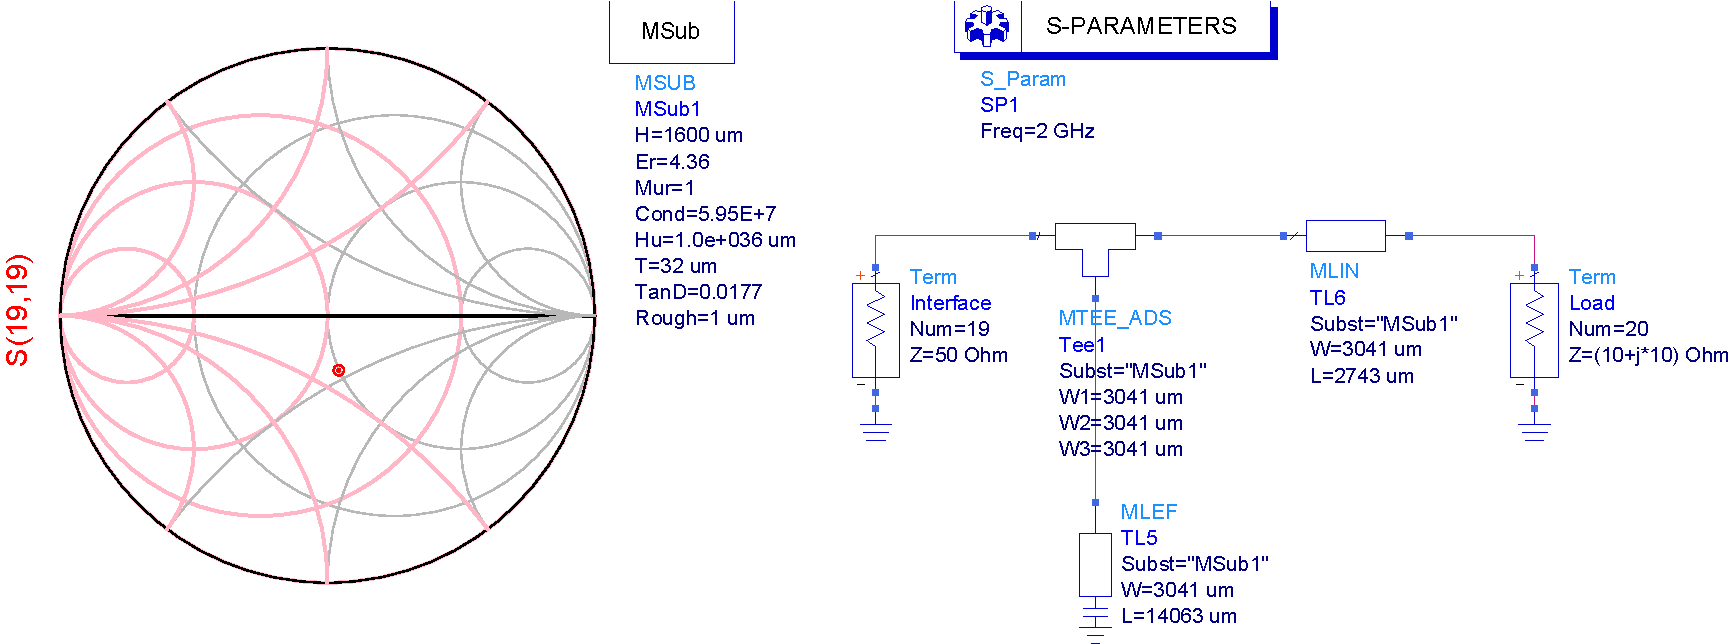
\includegraphics[width=16cm]{StubRe1}
\caption{Rete di adattamento con stub reale.}
\label{fig:StubRe1}
\end{figure}

Anche in questo caso come negli altri, essendo un adattamento reale, il risultato ottenuto non coincide con un minimo del coefficiente di riflessione a 2 GHz. Tramite l'utilizzo della funzione di \itt{tuning} sulle lunghezze delle microstrisce siamo quindi andati a trovare i parametri fisici ottimali per la rete di adattamento che differiscono da quelli trovati con {LineCalc} poich� tengono in considerazione le perdite dovute al caso reale (fig. \ref{fig:StubRe2}).

\begin{figure}[ht!]
\centering % \hspace{2cm}
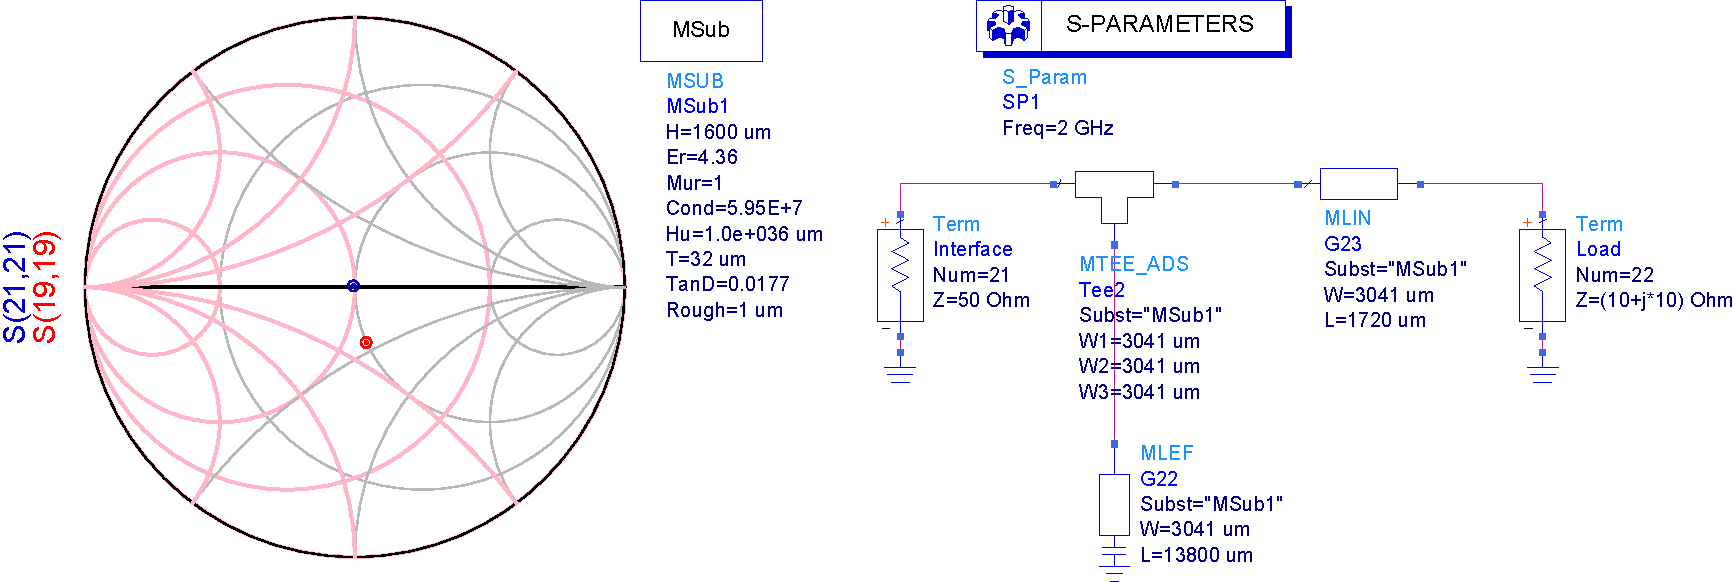
\includegraphics[width=16cm]{StubRe2}
\caption{Rete di adattamento con stub reale ottimizzata.}
\label{fig:StubRe2}
\end{figure}

Il risultato dell'operazione ha determinato una modifica sostanziale della lunghezza fisica del componente MLIN, portata da {2743 $\mu$m} a {1720 $\mu$m}, mentre MLEF � passato da {14063 $\mu$m} a {13800 $\mu$m}. Il notevole guadagno di questa operazione pu� essere facilmente osservato in figura \ref{fig:StubReBand} ove vengono mostrate le risposte in frequenza delle due reti; in blu si pu� notare come la rete ottimizzata abbia una banda di adattamento maggiore e pi� centrata alla frequenza di 2 GHz.

\begin{figure}[ht!]
\centering % \hspace{2cm}
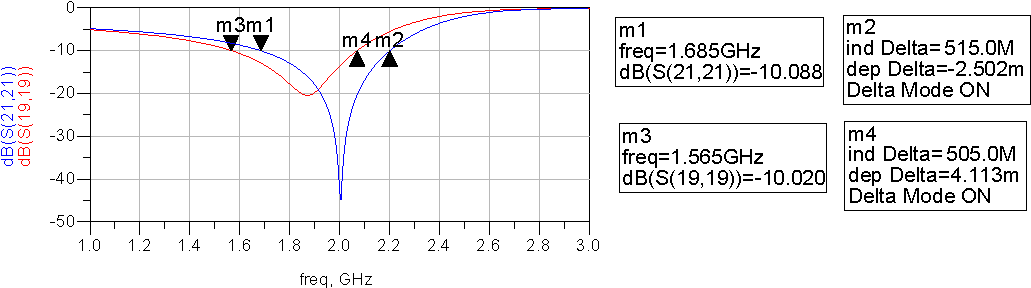
\includegraphics[width=12cm]{StubReBand}
\caption{Bande dell'adattamento reale con stub.}
\label{fig:StubReBand}
\end{figure}

\subsection{\texorpdfstring{ Trasformatore a $\lambda / 4$}{ Trasformatore a Lambda Quarti}}

\par Per realizzare il trasformatore a $\lambda / 4$ reale sono state utilizzate linee a microstriscia MLIN basate su un substrato modellato tramite il componente MSUB.
 
\begin{figure}[ht!]
\centering % \hspace{2cm}
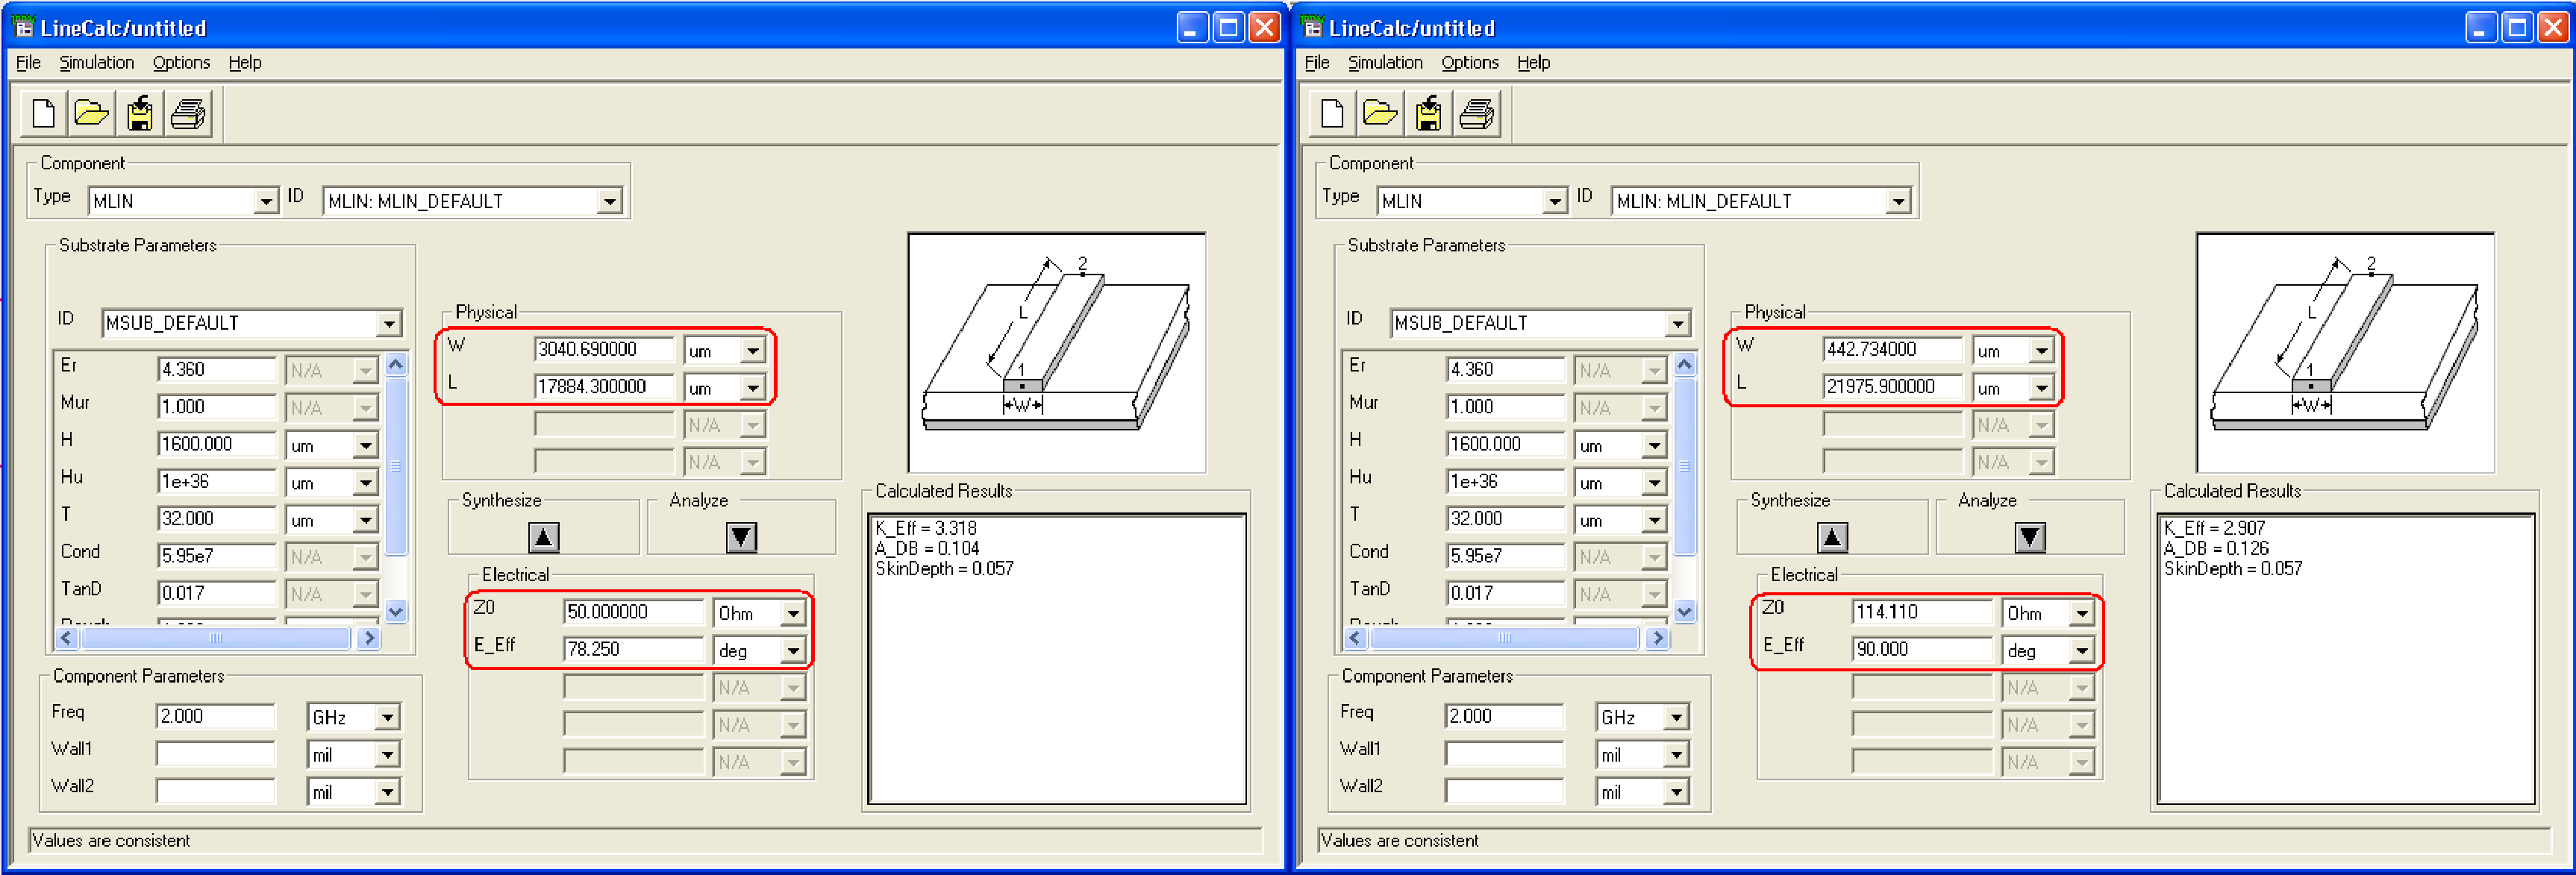
\includegraphics[width=16cm]{LineCalcLambda4th}
\caption{Utilizzo del tool LineCalc per trovare i parametri fisici.}
\label{fig:LineCalcLambda4th}
\end{figure}

Il modello circuitale di riferimento � quello analizzato nel paragrafo \ref{sec:Lambda4th} in figura \ref{fig:Lambda4th1Band}, ovvero un tratto di linea lungo 78,25 gradi elettrici e di impedenza 50 $\Omega$ che rende il carico puramente reale, ed un tratto di linea lungo $\lambda / 4$ (90 gradi elettrici) di impedenza 114,11 $\Omega$ che completo l'adattamento portando il carico al centro della carta di Smith. Tutto questo � stato riportato al caso reale utilizzando due componenti di tipo MLIN, mediante l'uso del \itt{tool LineCalc} abbiamo calcolato i parametri fisici derivati da quelli elettrici a nostra conoscenza (Vedi fig. \ref{fig:LineCalcLambda4th}). Tali parametri sono quindi stati riportati al modello in microstriscia, introducendo il componente MSTEP che tiene conto degli effetti parassiti introdotti dalla discontinuit� tra MLIN e il tratto a $\lambda / 4$ (Vedi fig. \ref{fig:Lambda4thRe}).

\begin{figure}[ht!]
\centering % \hspace{2cm}
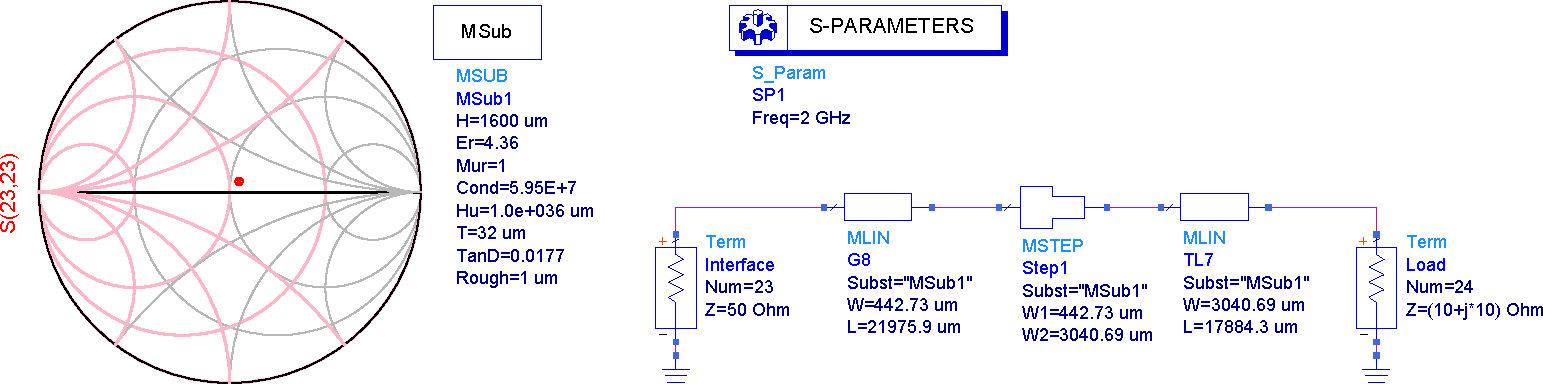
\includegraphics[width=16cm]{Lambda4thRe}
\caption{Rete di adattamento con trasformatore a $\lambda / 4$ reale.}
\label{fig:Lambda4thRe}
\end{figure}

Siamo quindi passati a graficare la risposta in frequenza della rete modellata (Vedi fig. \ref{fig:Lambda4thReBand}).
In quest'ultimo caso non si � reso necessario effettuare un'operazione di ottimizzazione in quanto il coefficiente di riflessione ottenuto � stato ritenuto sufficientemente buono per gli obiettivi di progetto. Inoltre la risposta in frequenza risulta essere abbastanza centrata e di poco migliorabile cos� come la banda. Possiamo notare che quest'ultima � la pi� stretta finora incontrata, ovvero {280 MHz}.

\begin{figure}[ht!]
\centering % \hspace{2cm}
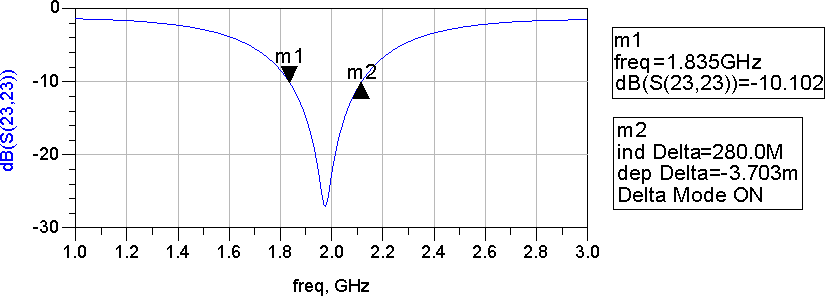
\includegraphics[width=12cm]{Lambda4thReBand}
\caption{Banda della rete di adattamento con trasformatore a $\lambda / 4$ reale.}
\label{fig:Lambda4thReBand}
\end{figure}

Dalle varie risposte in frequenza fin qui analizzate possiamo notare come gli adattamenti reali non riescano ad arrivare ad una attenuazione della riflessione pari a quella delle reti ideali poich� i componenti reali introducono numerosi fattori parassiti che non permettono di ottenere gli stessi risultati.

\newpage
\section{Riepilogo grafico e tabulare dei risultati ottenuti}
\begin{figure}[ht!]
\centering % \hspace{2cm}
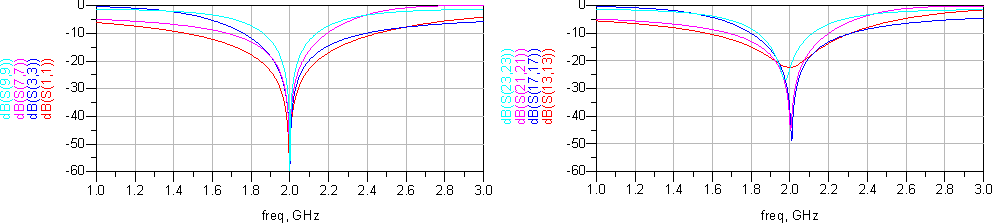
\includegraphics[width=16cm]{Bands}
\begin{tabular}{|c c c c c c|}
\hline
{Coefficiente} & {Posizione} & {Tipologia} & {Colore} & {Rete di} & {Banda di } \\
{di riflessione} & {grafico} & {di adattamento} & {} & {adattamento} & {adattamento} \\
\hline
{S(1,1)} & {Sinistra} & {Ideale} & {rosso} & {L (ISCP)} & {985 MHz} \\
{S(3,3)} & {Sinistra} & {Ideale} & {blu} & {L (CSIP)} & {630 MHz}\\
S(7,7) & Sinistra & Ideale & magenta & Stub & 510 MHz \\
S(9,9) & Sinistra & Ideale & ciano & $\lambda / 4$ & 270 MHz \\
S(13,13) & Destra & Reale (opt) & rosso & L (ISCP) & 750 MHz \\
S(17,17) & Destra & Reale (opt) & blu & L (CSIP) & 510 MHz \\
S(21,21) & Destra & Reale (opt) & magenta & Stub & 515 MHz \\
S(23,23) & Destra & Reale & ciano & $\lambda / 4$ & 280 MHz \\
\hline 
\end{tabular}
\caption{Risposte in frequenza delle reti di adattamento.}
\label{fig:Bands}
\end{figure}

\graphicspath{{img/lab2/}}
\chapter{Rivelatore di potenza}

\par Prima di progettare la struttura vera e propria di un transceiver, in questo secondo capitolo siamo andati a analizzare un altro dispositivo, ormai presente all'interno della maggior parte dei transceiver commerciali, ovvero il power detector, o signal detector. Come suggerisce il nome, questo circuito � in grado di rilevare un segnale in termini di potenza, traducendone il livello di potenza in uno di tensione sufficientemente alto da poter essere trattato. In questo modo, rilevando il valore di potenza del segnale sull'antenna � possibile regolare direttamente i guadagni degli amplificatori di tutta la catena di ricezione, attraverso un circuito di controllo automatico del guadagno (\itt{Automatic Gain Control}, AGC). Questo dispositivo � in grado di variare l'amplificazione del segnale ricevuto affinch� resti il pi� costante possibile passando per i vari blocchi della catena di ricezione, evitando una distorsione del segnale. Gli AGC sono integrati non solo nei telefoni cellulari ma anche nei microchip degli impianti video.

\par Tornando al power detector, anch'esso � presente in forma integrata nei sistemi di telecomunicazioni moderni e viene progettato per lavorare a tutte le frequenze di interesse degli standard di comunicazione emergenti (WLAN, UWB, GSM, UMTS, Bluetooth e il WiMAX). Trattandosi di un dispositivo piuttosto versatile possiede svariate applicazioni, anche in campi meno
``pubblicizzati''. Sfruttando infatti il principio che sta alla base del signal detector, cio� la rivelazione di segnali a delle particolari frequenze di interesse, viene utilizzato nel campo della sicurezza e della privacy, ad esempio per rilevare la presenza di cellulari (fig. \ref{fig:signaldetector}), microspie o telecamere wireless nascoste. Altra applicazione suggestiva � il cosiddetto \itt{phone cell jammer}, dispositivo in grado di generare disturbi su un dato apparecchio telefonico mobile una volta individuato proprio attraverso il power detector (fig. \ref{fig:cellphonejammer}).

\begin{figure}[ht!]
\centering % \hspace{2cm}
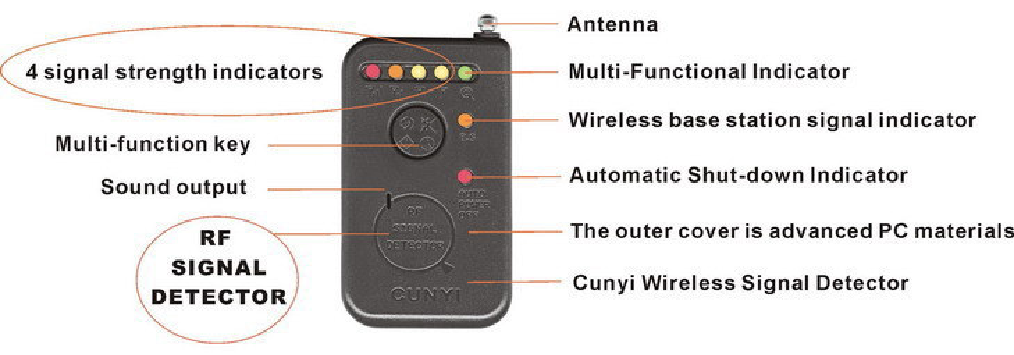
\includegraphics[width=12cm]{signaldetector}
\caption{Signal Detector.}
\label{fig:signaldetector}
\end{figure}

 
\begin{figure}[ht!]
\centering % \hspace{2cm}
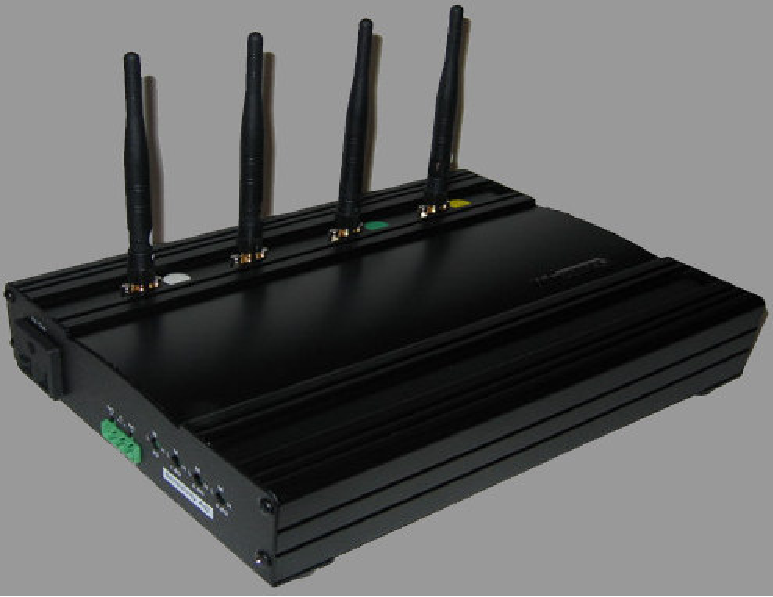
\includegraphics[width=12cm]{cellphonejammer}
\caption{Cell Phone Jammer.}
\label{fig:cellphonejammer}
\end{figure}

%\newpage

\section{Scopo e descrizione dell'esperienza}

A parte queste applicazioni pi� particolari, lo scopo della nostra esercitazione � stato la progettazione di un circuito power detector base, per la sola frequenza di lavoro di 868 MHz, il cui schema a blocchi fondamentali � rappresentato in figura \ref{fig:schema}. La rilevazione del segnale � a soglia : un comparatore genera un livello alto in uscita qualora la potenza del segnale RF abbia superato un determinato livello.

\begin{figure}[ht!]
\centering % \hspace{2cm}
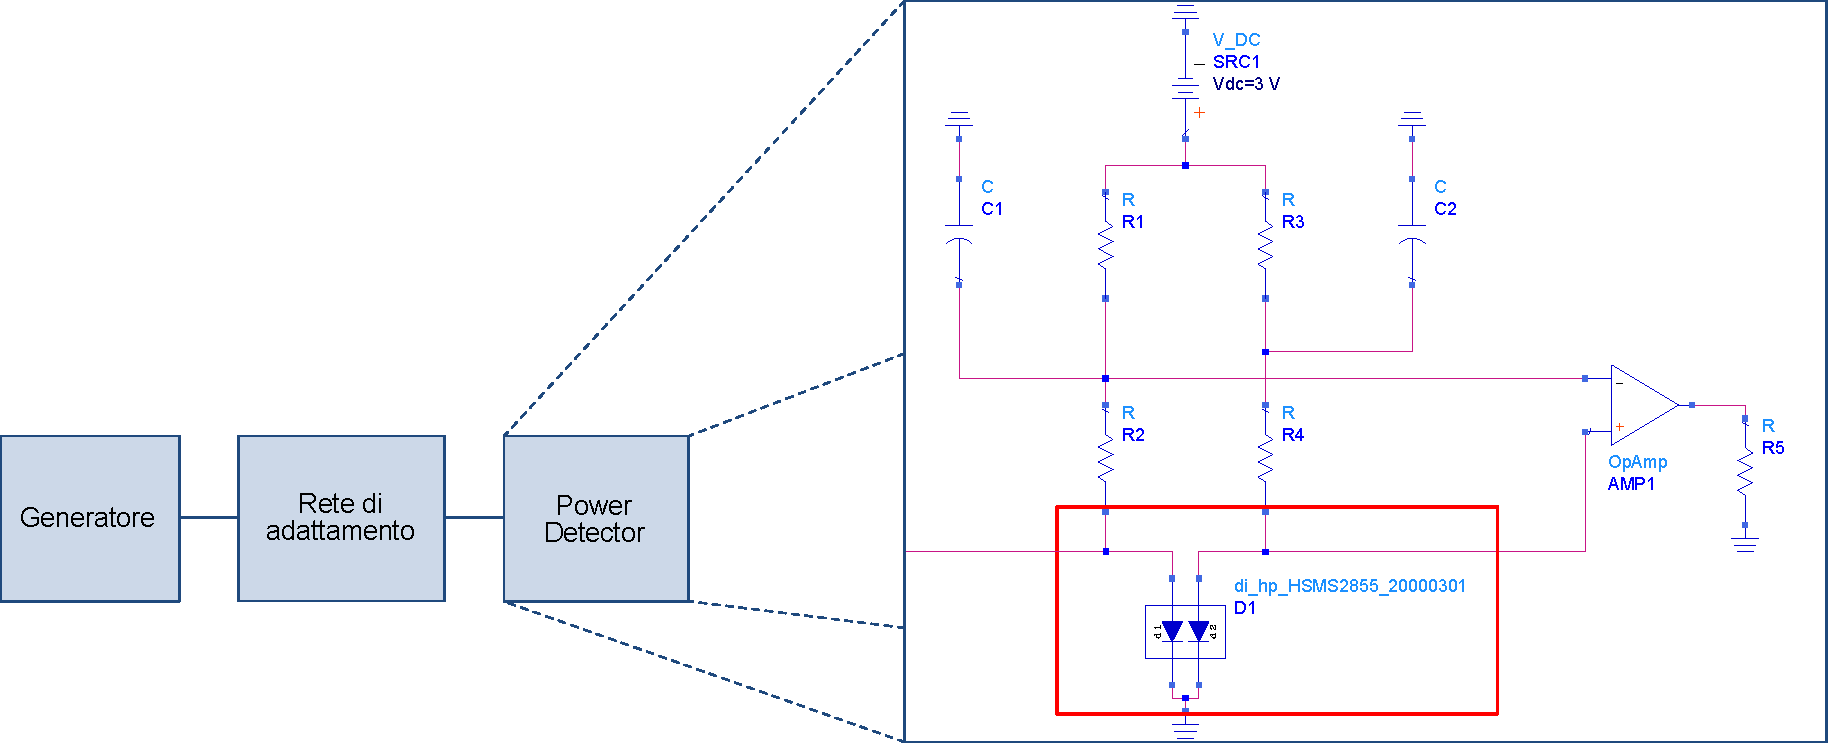
\includegraphics[width=16cm]{schema}
\caption{Schema a blocchi del power detector.}
\label{fig:schema}
\end{figure}

\section{Il diodo HSMS2855: caratteristiche tecniche e curve corrente-tensione}

\par Come si nota dalla figura \ref{fig:schema} abbiamo una rete di adattamento prima del circuito vero e proprio, il cui cuore, l'elemento fondamentale, � il diodo HSMS serie 285x della Agilent Technologies, in particolare il modello 2855, caratterizzato da un contenitore SOT-143 a montaggio superficiale, al cui interno � presente una coppia di diodi paralleli separati tra loro (\itt{unconnected pair}, fig. \ref{fig:sot143}) . 
 
\begin{figure}[ht!]
\centering % \hspace{2cm}
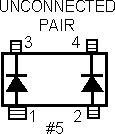
\includegraphics[scale=1]{sot143}
\caption{Package SOT 143 della coppia di diodi HSMS2855.}
\label{fig:sot143}
\end{figure}

\par La scelta dei due diodi � dettata da ragioni di simmetria e bilanciamento dell'intero circuito, cos� come accadr� per la rete di polarizzazione a 4 resistori descritta in seguito. La famiglia di diodi {Schottky} \itt{zero bias} (cio� con polarizzazione intorno all'origine) HSMS-285x � stata progettata e ottimizzata per applicazioni nel campo dei piccoli segnali ($\mathrm{P}_\mathrm{IN}$ < -20 dBm) e per frequenze inferiori ad 1,5~GHz \cite{HSMS}. Essendo diodi rilevatori zero bias, sono ideali per applicazioni RF/ID e RF Tag, prive di alimentazione primaria; inoltre forniscono un'elevata sensibilit� di rivelazione (oltre 50 mV/$\mu$W a 915 MHz). Le configurazioni stesse dei package disponibili non sono lasciate al caso e, attraverso opportune tecniche di fabbricazione, garantiscono il pi� alto grado possibile di matching fra i due diodi realizzati all'interno dello stesso package, uno dei requisiti fondamentali per l'intera struttura da progettare. Ovviamente il datasheet, oltre alle caratteristiche tecniche fornisce anche tutti i parametri SPICE da utilizzare per implementare il modello non lineare del diodo in qualsiasi simulatore commerciale. Nel nostro caso, il diodo HSMS285x � un prodotto della Agilent Technologies, il cui modello � gi� inserito nelle librerie presenti su ADS. In figura \ref{fig:IVcaratt} viene illustrata la caratteristica corrente-tensione (I-V) dei diodi ed il circuito che ne ha permesso l'analisi.

% nella prima parte dell'esercitazione quindi siamo andati a verificare che il comportamento del componente fornito dal software coincidesse con i valori tabulati sul datasheet, ovvero 150 $\mu$A a 100 mV. Effettivamente, (fig. 5) i valori simulati sono proprio quelli desiderati.
 
\begin{figure}[ht!]
%\centering % \hspace{2cm}
\begin{minipage}[b]{0.5\linewidth} % A minipage that covers half the page
\centering
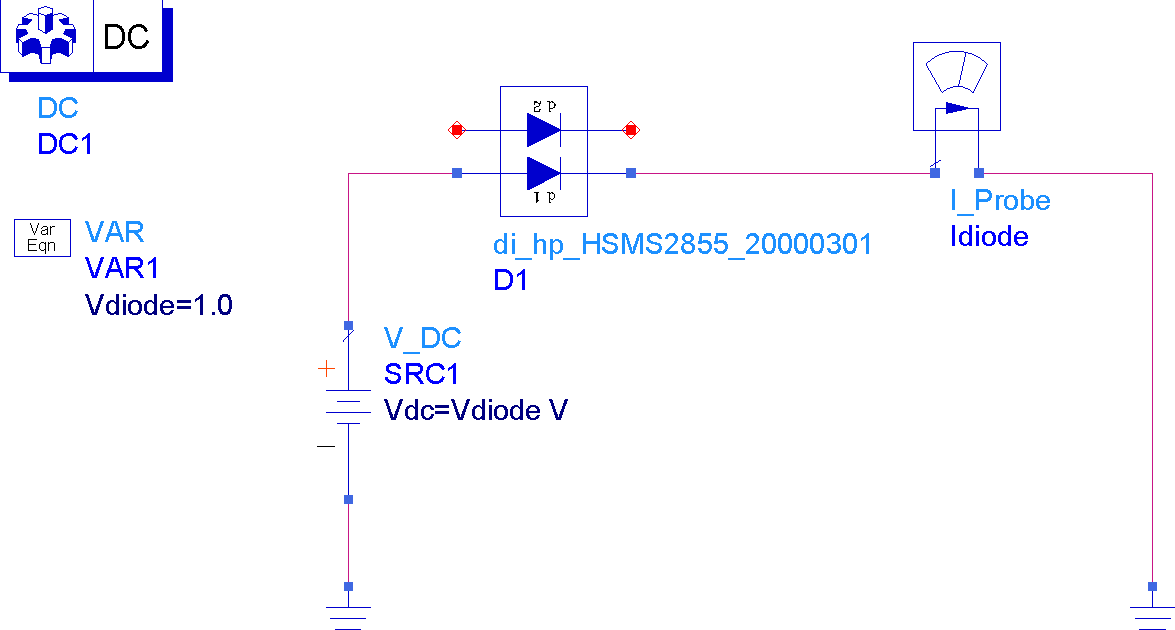
\includegraphics[width=8cm]{IVcarattschem}

\end{minipage}
\hspace{0.5cm} % To get a little bit of space between the figures
\begin{minipage}[b]{0.5\linewidth}
\centering
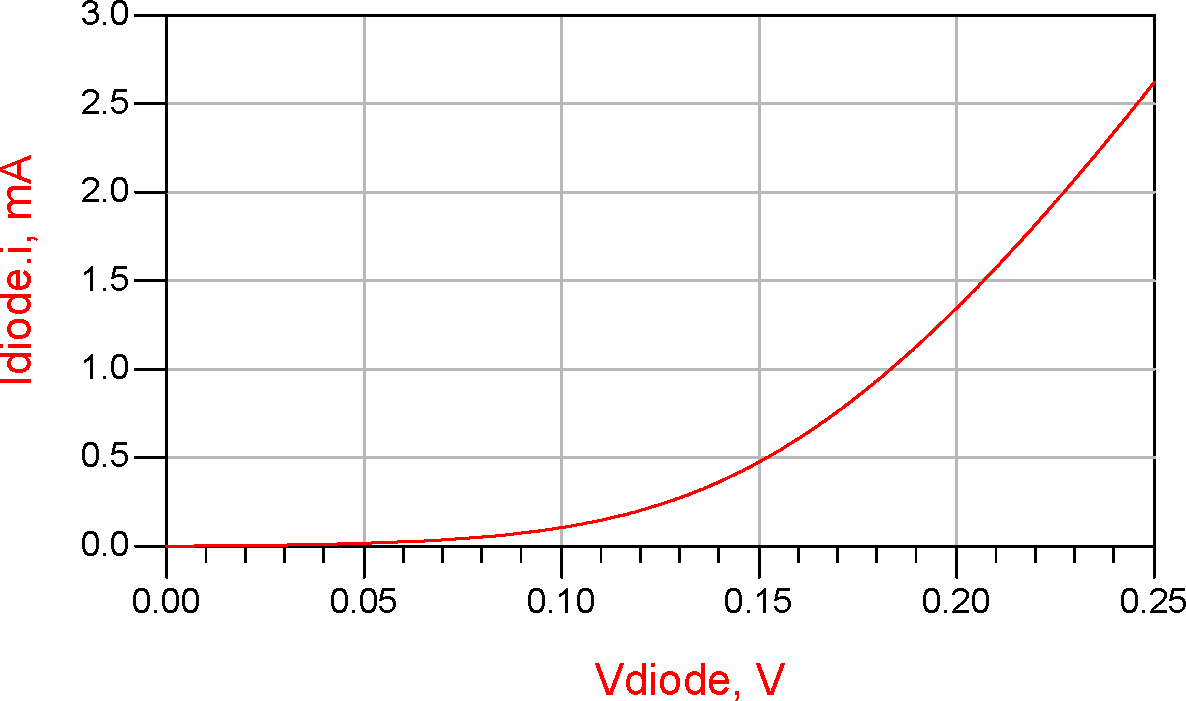
\includegraphics[width=7cm]{IVcaratt} 
%\caption{En liten bild till}
\end{minipage}
\caption{Caratteristica I-V.}
\label{fig:IVcaratt}
\end{figure}

\subsubsection*{Simulatore \itt{DC}}

\par Per ottenere il grafico di figura \ref{fig:IVcaratt}, non abbiamo fatto altro che studiare il punto di lavoro del nostro \itt{device under test} (DUT) attraverso un'analisi di tipo DC \cite{DC}, alla base di ogni simulazione analogica e a radiofrequenza. Il simulatore segue tutta una serie di passi: inizialmente esegue un controllo della topologia del circuito prima dell'analisi vera e propria del punto di lavoro in continua. Il simulatore permette anche, come nel nostro caso, di variare uno o pi� parametri (attraverso un \itt{parameter sweep}), in modo da rappresentare le curve I-V di dispositivi non lineari quali diodi o transistor ad esempio. Il controllo della topologia del circuito permette di trovare ed eliminare gli errori pi� comuni e banali (ad esempio la presenza di nodi degeneri) che porterebbero a errori ben pi� gravi nel corso della simulazione (riportati poi nella finestra \itt{Simulation/Synthesis Messages}). Invece durante l'analisi DC, il simulatore calcola la risposta di un dato circuito ad un particolare stimolo, convertendo, a partire da opportune ipotesi, un sistema di equazioni differenziali ordinarie non lineari in un sistema di equazioni algebriche non lineari, e risolvendole poi numericamente. 
\par Il punto cruciale su cui si basano questi CAD si trova proprio in questo complicato passaggio di equazioni: ogni simulatore infatti converte le equazioni differenziali in equazioni algebriche in modo diverso dagli altri e utilizza un particolare metodo numerico per la risoluzione delle equazioni algebriche ottenute. In questo modo nascono la maggior parte delle simulazioni gi� elencate per ADS, ovvero la \itt{DC}, la \itt{AC}, la \itt{S-parameter}, la \itt{Transient}, l'\itt{Harmonic Balance} e la \itt{Circuit Envelope}. Le tecniche numeriche di simulazione si appoggiano su svariati processi di iterazione per ottenere la convergenza matematica verso un punto di equilibrio nelle equazioni algebriche non lineari che descrivono il circuito. Una volta raggiunto il punto di equilibrio entro certi valori di tolleranza, si ottiene una soluzione; questo implica che talvolta, come ci � capitato nel corso delle esercitazioni, il simulatore non riesce a convergere e a fornire una soluzione. Questo pu� essere dovuto sia alla scelta non opportuna del metodo di convergenza, sia a dei vincoli sulle tolleranze di default troppo stringenti. %; sta a noi decidere in che modo privilegiare un aspetto o l'altro. Alcune delle tecniche di convergenza pi� importanti sono l'algoritmo Newton-Raphson, il source-level sweeping, l'arc-length continuation, il Gmin relaxation, e l'analisi pseudo-transient. Come gi� accennato � possibile cambiare diversi parametri sulla tolleranza, rendendoli meno vincolanti per ottenere la convergenza del simulatore a discapito di un risultato meno accurato (Current relative tolerance (\textsf{I{\textunderscore}RelTol}), Voltage relative tolerance (V{\textunderscore}RelTol), Current absolute tolerance (I{\textunderscore}AbsTol), Voltage absolute tolerance (V{\textunderscore}AbsTol)). Da notare che le equazioni utilizzate per controllare la convergenza sono applicate a tutti i tipi di analisi, non solo alla DC, come vedremo meglio in seguito.


\section{Descrizione del circuito di rivelazione} \label{sec:CircRiv}

\par Una volta verificate le curve I-V del diodo, abbiamo realizzato lo schematico del power detector (vedi fig. \ref{fig:rete100}), lasciando da parte per ora la rete di adattamento gi� presente in figura \ref{fig:schema}. Inizialmente abbiamo cercato di ottimizzare il circuito in modo da rilevare un livello di potenza il pi� basso possibile; solo in seguito aggiungeremo la rete di adattamento pi� opportuna in grado di diminuire ulteriormente la soglia di rilevazione.
\begin{figure}[ht!]
\centering % \hspace{2cm}
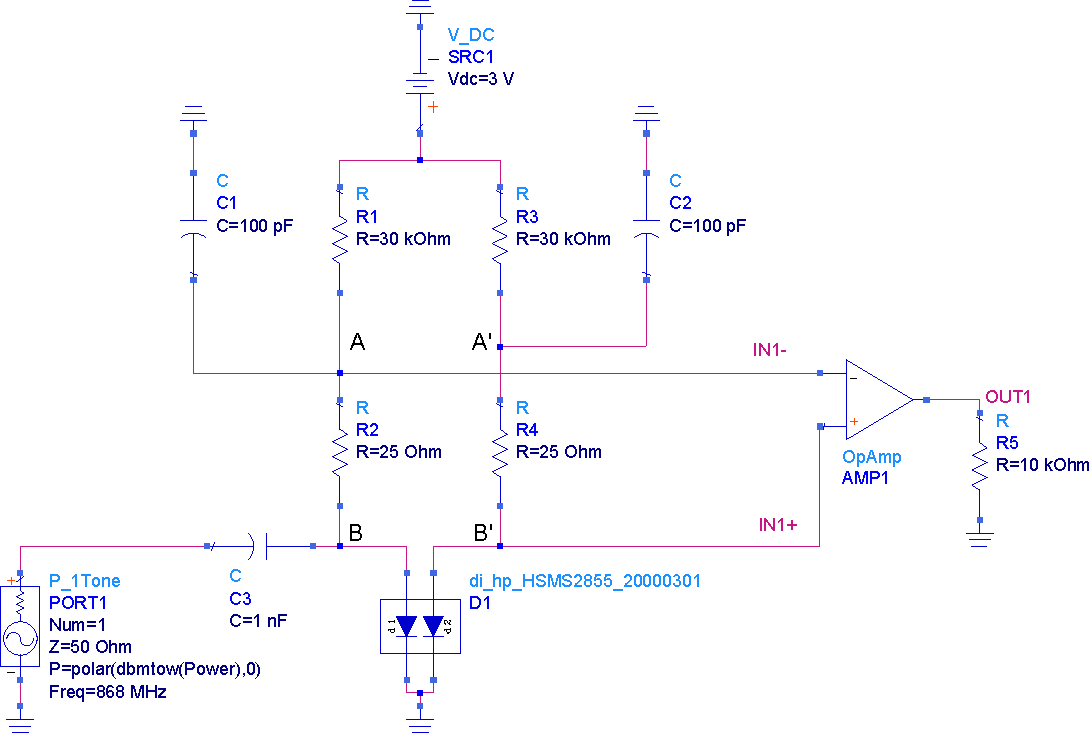
\includegraphics[width=15cm]{rete100}
\caption{Schema elettrico del power detector.}
\label{fig:rete100}
\end{figure}
Il circuito di figura \ref{fig:rete100} � caratterizzato da una rete di polarizzazione simmetrica a 4 resistori, a due a due identici ($\mathrm{R}_1 = \mathrm{R}_3$ e $\mathrm{R}_2 = \mathrm{R}_4$), configurazione in grado di regolare la soglia di rilevazione del dispositivo. In effetti, le resistenze $\mathrm{R}_1$ e $\mathrm{R}_3$ determinano la corrente di polarizzazione dei diodi Schottky, essendo le resistenze $\mathrm{R}_2$ e $\mathrm{R}_4$ di valore ad esse trascurabile: la limitazione della corrente di polarizzazione � quindi principalmente dovuta alle resistenze $\mathrm{R}_1$ e $\mathrm{R}_3$. Lo scopo delle resistenze $\mathrm{R}_2$ e $\mathrm{R}_4$ � quello di mantenere, in assenza di segnale RF da rivelare, l'uscita del comparatore a livello basso. Vista la simmetria della rete di resistenze e dei diodi \itt{matched}, le tensioni ai nodi A e A', cos� come in B e B', sono pressoch� identiche ($V_\mathrm{A} \cong V_\mathrm{A'}$ e ${V_\mathrm{D}}_1 = V_\mathrm{B} \cong {V_\mathrm{D}}_2 = V_\mathrm{B'}$, gli scostamenti sono dovuti alle tolleranze costruttive dei componenti) e la tensione differenziale $V_\mathrm{DIFF} = V_\mathrm{IN1+} - V_\mathrm{IN1-} = V_\mathrm{A} - V_\mathrm{B'} \cong V_\mathrm{A} - V_\mathrm{B} \cong V_\mathrm{A'} - V_\mathrm{B'}$ viene quindi impostata, nota la corrente che scorre nei rami di polarizzazione ($I_\mathrm{1} \cong \frac{V_\mathrm{DC} - {V_\mathrm{D}}_1}{\mathrm{R}_1} \cong I_\mathrm{2}$), dal valore delle resistenze $\mathrm{R}_2$ e $\mathrm{R}_4$ ($V_\mathrm{DIFF} \cong \mathrm{R}_2 \cdot I_1 \cong \mathrm{R}_4 \cdot I_2$). Visto il verso delle correnti di polarizzazione, la caduta sulle resistenze $\mathrm{R}_2$ e $\mathrm{R}_4$ � positiva, mantenendo quindi $V_\mathrm{DIFF}$ negativa per un livello basso in uscita. 
A fronte di un segnale RF sinusoidale (tono a 868 MHz), il diodo $\mathrm{D}_1$ entra in conduzione per la sola semionda positiva presentando il comportamento di un cortocircuito e limitando quindi la tensione al nodo B, mentre la semionda negativa rimane pressoch� inalterata ai capi del diodo. \`E proprio questo meccanismo di distorsione del segnale RF che permette al comparatore di percepire una $V_\mathrm{DIFF}$ positiva : via via che la potenza aumenta, il valor medio (componente DC) del segnale al nodo B tende a valori negativi, di ampiezza sempre maggiore (fig. \ref{fig:distorsione}).
\begin{figure}[ht!]
\centering % \hspace{2cm}
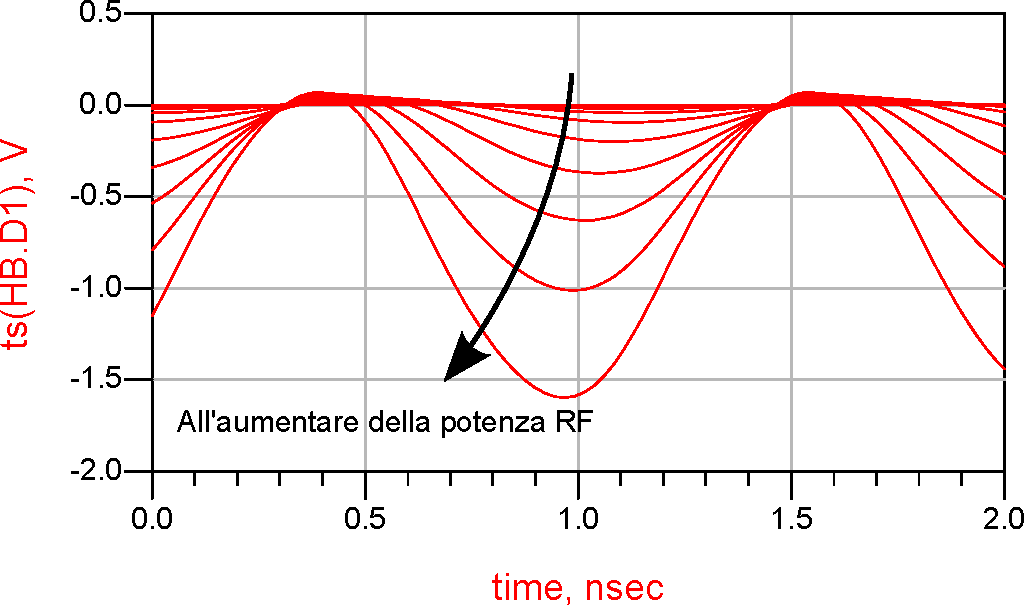
\includegraphics[width=10cm]{distorsione}
\caption{Tensione ai capi del diodo $\mathrm{D}_1$ ($V_\mathrm{B}$).}
\label{fig:distorsione}
\end{figure}
Ad un determinato livello di potenza in ingresso, la tensione al nodo A, seguendo l'andamento del nodo B, eguaglier� la tensione in B', portando poi a livello alto l'uscita del comparatore per un livello di potenza leggermente superiore. I condensatori $\mathrm{C}_1$ e $\mathrm{C}_2$ servono essenzialmente a cortocircuitare il segnale RF e le sue armoniche prodotte dalla caratteristica non lineare del diodo, mantenendo le tensioni ai nodi A e A' costanti. Inoltre, l'effetto passa basso (con costante di tempo di scarica di $\mathrm{C}_\mathrm{1}$ $\approx \ \mathrm{R}_2 \cdot \mathrm{C}_1$) che introducono questi condensatori regola il tempo di risposta del power detector a fronte di un'impulso di potenza rilevabile, implicando una durata minima dell'impulso per poter essere effettivamente rilevato.
\par La precedente descrizione del power detector introduce il procedimento adottato per studiare il circuito col programma ADS: prima infatti abbiamo realizzato uno sweep in potenza per ricavare la soglia di attivazione del comparatore ed infine abbiamo studiato il circuito al transitorio per vedere quanto velocemente potesse scaricarsi il condensatore $\mathrm{C}_1$ per portare a livello alto l'uscita del comparatore.

%\newpage
\section{Scelta della rete di polarizzazione} \label{sec:retpol}

\par Innanzitutto siamo andati a dimensionare opportunamente i quattro resistori per ricavare una rete di polarizzazione con una corrente sui rami simmetrici di circa 100 $\mu$A, per polarizzare il diodo al valore indicato dal datasheet e abbiamo ottenuto i valori mostrati in figura \ref{fig:rete1002}. 
\begin{figure}[ht!]
\centering % \hspace{2cm}
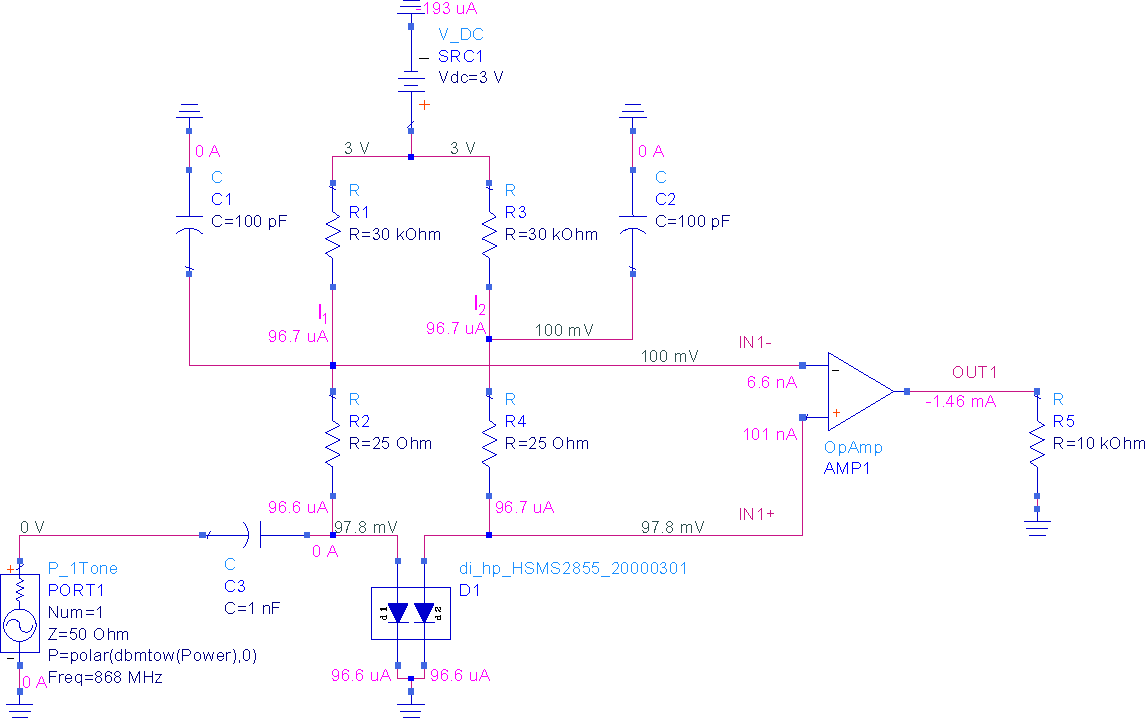
\includegraphics[width=15cm]{rete1002}
\caption{Rete di polarizzazione dei diodi a 100 $\mu$A.}
\label{fig:rete1002}
\end{figure}
Per visualizzare i valori di corrente e tensione e controllare se davvero coincidevano con quelli ottenuti dai calcoli, abbiamo sfruttato il comando \textsf{annotate DC simulation}, dopo aver eseguito la simulazione DC. Poi abbiamo effettuato appunto uno sweep in potenza da -50 a 10 dBm col generatore a singolo tono, andando a rappresentare in un grafico la variazione delle tensioni sui due morsetti del comparatore al variare della potenza in ingresso, per ricavare il valore di soglia in potenza. Stesso procedimento � stato effettuato anche per altri due valori di corrente di polarizzazione, rispettivamente 50 $\mu$A e 150 $\mu$A. Questi ulteriori tentativi sono stati realizzati per cercare la corrente di polarizzazione che garantisse la sensibilit� migliore, ed i dati trovati sono stati raccolti nella tabella \ref{tab:retpol}.

\begin{table}[ht!]
\centering
\begin{tabular}{|c|ccccccccc|}
\hline
\ & $\mathrm{I}_1$ [$\mu$A] & $\mathrm{I}_2$ [$\mu$A] & $\mathrm{V-}$ [mV] & $\mathrm{V+}$ [mV] & $\mathrm{R}_1$ [k$\Omega$] & $\mathrm{R}_2$ [$\Omega$] & $\mathrm{R}_3$ [k$\Omega$] & $\mathrm{R}_4$ [$\Omega$] & Soglia [dBm] \\ \hline % \hline
50 $\mu$A & 48,6 & 48,6 & 81,1 & 78,7 & 60 & 50 & 60 & 50 & -25 \\
100 $\mu$A & 96,7 & 96,7 & 100 & 97,8 & 30 & 25 & 30 & 25 & -21 \\
150 $\mu$A & 144 & 144 & 112 & 110 & 20 & 15 & 20 & 15 & -18 \\ \hline
\end{tabular}
\label{tab:retpol}
\caption{Reti di polarizzazione e variazione della soglia di rilevazione.}
\end{table}

Come si pu� notare la sensibilit� migliore, pari a -25 dBm, (vedi fig. \ref{fig:retpol}) si ottiene con una corrente di polarizzazione di 50 $\mu$A, inferiore a quella fornita dal datasheet; abbiamo quindi proseguito su questa strada per migliorare ulteriormente la sensibilit� variando la rete di polarizzazione per ottenere correnti inferiori a 50 $\mu$A.

\begin{figure}[ht!]
\centering % \hspace{2cm}
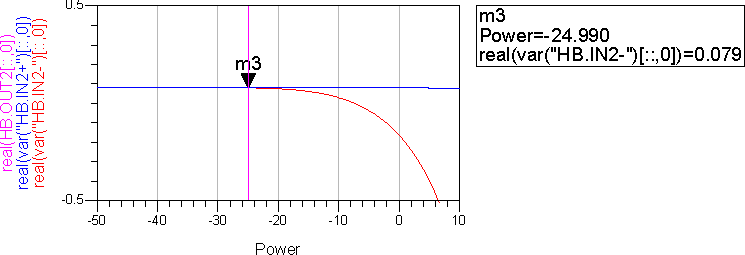
\includegraphics[width=15cm]{retpol}
\caption{Sweep in potenza per la rete di polarizzazione a 50 $\mu$A.}
\label{fig:retpol}
\end{figure}

Prima di passare al punto successivo per� torniamo un attimo indietro per spiegare come abbiamo ottenuto il grafico di fig. \ref{fig:retpol}. Effettivamente tutti i valori di soglia ed il grafico stesso sono stati ricavati applicando un altro tipo di simulazione molto importante, la cosiddetta \itt{Harmonic Balance}.

%\newpage
\subsubsection*{Simulatore \itt{Harmonic Balance}}

\par Harmonic Balance � una tecnica di analisi molto accurata che opera direttamente nel dominio della frequenza, risultando molto pi� veloce di un'analisi completa di tipo \itt{Transient}. L'Harmonic Balance � la scelta naturale per studiare problemi a radiofrequenza e a microonde, sia perch� lavora in frequenza ma anche perch� permette di ottenere rapidamente parametri fondamentali quali i punti di intercetta del terzo ordine, la distorsione armonica totale (THD) e le componenti di distorsione relative ai prodotti di intermodulazione, oltre a supportare un'analisi del rumore di tipo non-lineare. Questo metodo di analisi assume come stimolo di ingresso alcune sinusoidi e la soluzione non � altro che una serie di queste sinusoidi comprendente sia le frequenze di ingresso che quelle relative alle altre armoniche significative ed ai termini di \itt{mixing}. Nel simulatore, il circuito viene rappresentato come un sistema di N equazioni differenziali ordinarie non lineari, dove N rappresenta la grandezza del circuito (numero di nodi e rami). Le sorgenti e le forme d'onda delle soluzioni sono approssimate attraverso i coefficienti di una serie di Fourier troncata. Un circuito con una solo sorgente di ingresso, come il nostro circuito, necessita di una simulazione Harmonic Balance a singolo tono, la cui soluzione avr� una forma del tipo :

\begin{equation}
v(t) = \mathit{Re} \left \{ \sum_{k = 0}^{K}  V_k e^{j2{\pi}kft} \right \} 
\end{equation}

Dove f � la frequenza fondamentale della sorgente, i $V_k$ sono i coefficienti di Fourier complessi calcolati dal simulatore (in tensione) e K determina il numero di armoniche utilizzate per la serie troncata ed � appunto chiamato \itt{ordine}. L'ordine deve essere abbastanza elevato in modo da garantire l'accuratezza della soluzione; tipicamente sono sufficienti tre armoniche per la maggior parte dei circuiti lineari, sette per quelli mediamente non lineari fino ad arrivare alle centinaia di armoniche per quelli fortemente non lineari caratterizzati ad esempio da fronti ripidi e \itt{spike}.
Nel caso pi� generale di sorgenti multiple avremo ovviamente come soluzione una serie multidimensionale, in cui ogni serie sar� riferita ad un diverso tono:

\begin{equation}
v(t) = \mathit{Re} \left \{ \sum_{k_1 = 0}^{K_1} \sum_{k_2 = 0}^{K_2} \cdots \sum_{k_n = 0}^{K_n} V_{k_1, k_2 \cdots k_n} e^{j2{\pi}(k_1 f_1 + \cdots + k_n f_n)t} \right \} 
\end{equation}
 

In questo caso � possibile regolare anche il parametro \textsf{MaxOrder}, relativo all'ordine massimo di termini mixed che vengono inclusi nella simulazione. I prodotti di mixing, o di intermodulazione, sono la combinazione di due o pi� frequenze fondamentali o delle loro successive armoniche; maggiore � il numero di sorgenti in gioco nel circuito da testare, pi� rapidamente crescono questi termini, che devono essere limitati per non appesantire troppo la simulazione.
La rappresentazione della soluzione tramite la serie di Fourier troncata trasforma il sistema di N equazioni differenziali non lineari in un sistema di N*M equazioni algebriche non lineari nel dominio della frequenza, dove M � il numero totale di frequenze inclusa la fondamentale, le loro armoniche e i prodotti di intermodulazione. Questo sistema di equazioni viene risolto attraverso il cosiddetto \itt{metodo di Newton} implementato nel risolutore \itt{non lineare} dell'HB. Il metodo di Newton consente di arrivare ad una soluzione attraverso iterazioni successive partendo da un passo iniziale ottenuto da una soluzione in continua del circuito.
\par Il sistema di equazioni algebriche non lineari � una rappresentazione nel dominio della frequenza della legge di Kirchhoff ai nodi (KCL), secondo la quale la somma delle correnti entranti in un nodo deve essere uguale alla somma delle correnti uscenti dal nodo stesso. La differenza tra questi due valori ad ogni iterazione del metodo di Newton � nota come \itt{residuo KCL}. Il risolutore non lineare di Newton (cos� come l'intera simulazione HB) riesce a convergere solo quando questo residuo � inferiore ad un valore di tolleranza che � possibile settare anche manualmente, variando di fatto l'accuratezza della simulazione. \`E possibile comunque sfruttare anche una soluzione di tipo Transient come passo iniziale, grazie alla \itt{Transient Assisted Harmonic Balance} (TAHB, automatica, pu� essere abilitata tra i parametri dell'HB). Questa simulazione garantisce uno \itt{starting point} molto pi� accurato della DC e quindi un residuo KCL finale inferiore, per questo � molto sfruttata per analizzare sistemi fortemente non lineari e contenenti forme d'onda a fronti ripidi, come i divisori. Il metodo di Newton genera un problema matriciale (sistema lineare di equazioni) ad ogni iterazione; questa matrice � jacobiana. In particolare � possibile scegliere non solo il numero massimo di iterazioni (\textsf{MaxIters}, per diminuire i requisiti di memoria),ma anche tre tipi di risolutori non lineari diversi, attraverso il parametro \textsf{ConvMode}. Mentre il risolutore \itt{Basic} abilita il metodo standard di Newton, per circuiti fortemente non lineari � possibile selezionare il risolutore \itt{Advanced}, molto pi� robusto; comunque di default viene settato il risolutore \itt{Auto} che combina le capacit� dei due precedenti. La matrice jacobiana ottenuta dal metodo di Newton viene poi fattorizzata grazie ad uno dei due possibili risolutori \itt{lineari} dell'HB: il \itt{Direct} ed il \itt{Krylov}. Mentre il primo utilizza metodi diretti di fattorizzazione della matrice (come l'eliminazione Gaussiana) per invertire la Jacobiana, il secondo sfrutta un metodo pi� sofisticato e risulta adatto a circuiti pi� complessi, essendo pi� veloce e meno dispendioso a livello di memoria richiesta (ma meno robusto). Come default per la fattorizzazione viene per� impostato un \itt{Auto Select Solver}, in grado di scegliere automaticamente il risolutore pi� adatto in base alla memoria RAM disponibile. 
\par Uno dei problemi affrontati durante l'esercitazione � stato appunto quello della convergenza non garantita a priori della nostra simulazione, come finora spiegato; � stato necessario dunque trovare dei possibili accorgimenti suggeriti dalla guida stessa del programma, per far operare correttamente la simulazione. Innanzitutto impostando l'ordine minimo richiesto per l'HB, cio� quattro armoniche, secondo le specifiche. Inoltre, poich� in HB i dispositivi non lineari vengono sovracampionati nel dominio del tempo, prima di passare al dominio della frequenza tramite FFT (\itt{Fast Fourier Transform}), pu� essere utile aumentare il parametro \textsf{Fundamental Oversample} per riuscire a campionare con maggiore precisione le forme d'onda del dispositivo. In questo modo non viene incrementato il numero di armoniche, ma solo la dimensione della FFT usata nell'HB, affinch� il circuito possa convergere pi� facilmente. Come ultima risorsa, abbiamo anche provato ad utilizzare il risolutore interno di tipo Krylov rispetto al Direct, settando opportunamente il \itt{preconditioner}, uno strumento in grado di alzare il tasso di convergenza, garantendo anche un risparmio sulla memoria. Di seguito in fig. \ref{fig:SchemHB} viene mostrato lo schema di funzionamento del simulatore HB.
 
\begin{figure}[ht!]
\centering % \hspace{2cm}
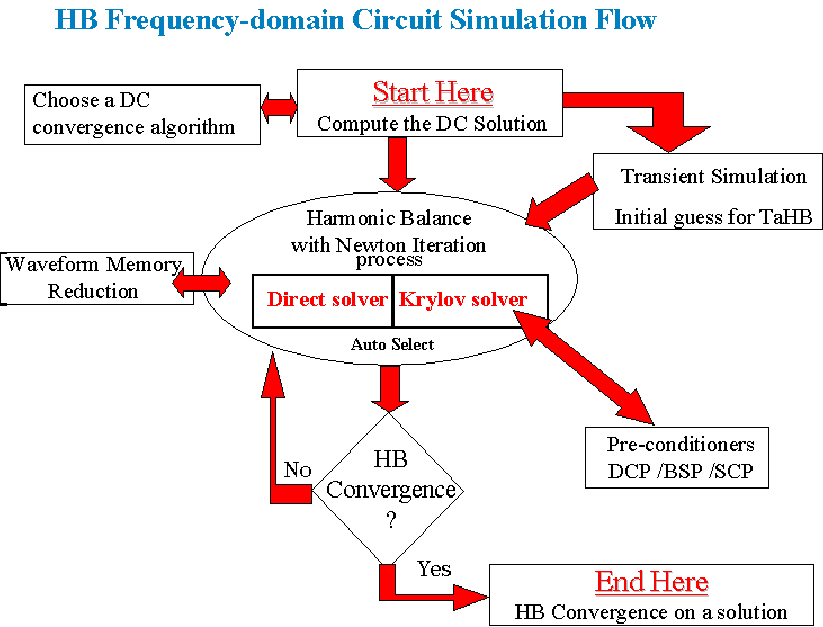
\includegraphics[width=15cm]{SchemHB}
\caption{Schema di funzionamento del simulatore HB.}
\label{fig:SchemHB}
\end{figure}

Dopo quanto detto andiamo a mostrare il settaggio dei nostri parametri per la HB e il generatore a singolo tono, con potenza variabile da -50 a 10 dBm, utilizzato per l'intera simulazione (vedi fig. \ref{fig:HBsim}).
 
\begin{figure}[ht!]
\centering % \hspace{2cm}
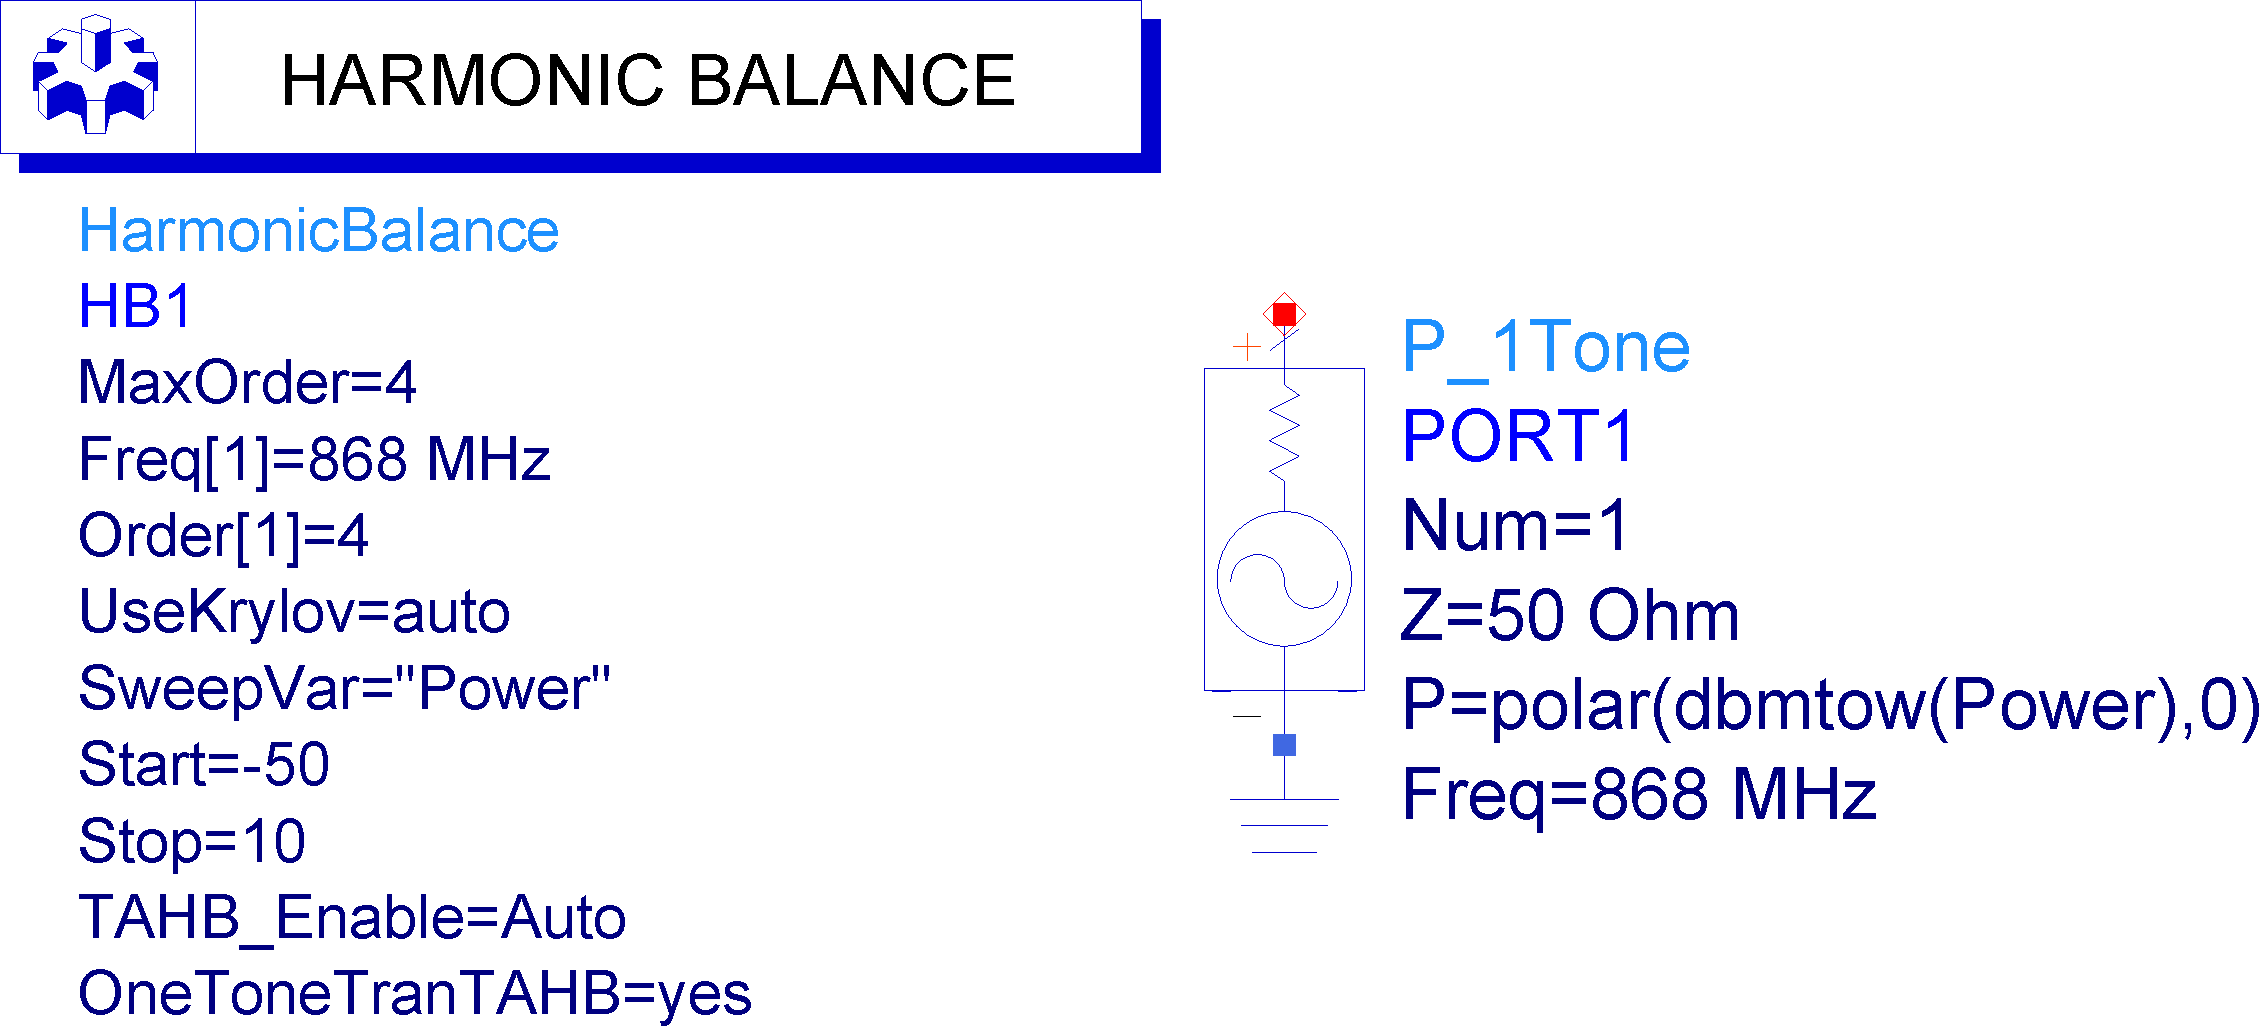
\includegraphics[width=10cm]{HBsim}
\caption{Setup dei parametri della simulazione HB.}
\label{fig:HBsim}
\end{figure}

\section{Valore di soglia ottimale}

\par Descritta la simulazione HB, passiamo ora al punto successivo, o per meglio dire l'obbiettivo da raggiungere, cio�, fissata una certa differenza di potenziale ai terminali del comparatore cercare di ottenere una soglia di rivelazione pi� bassa possibile. La tensione in ingresso al comparatore scelta � di circa 2 mV, valore che garantisce una bassa sensibilit� al rumore e ad eventuali tolleranze dei componenti. Per riuscire nell'intento siamo andati a variare opportunamente i valori dei 4 resistori di polarizzazione (mantenendo sempre la simmetria dei rami), fino a ottenere una soglia di circa -33 dBm con questi valori(fig. \ref{fig:-33dBm}).

\begin{figure}[ht!]
\centering % \hspace{2cm}
\includegraphics[width=14cm]{-33dBm}
\begin{tabular}{|ccccccccc|}
\hline
$\mathrm{I}_1$ [nA] & $\mathrm{I}_2$ [nA] & $\mathrm{V-}$ [mV] & $\mathrm{V+}$ [mV] & $\mathrm{R}_1$ [M$\Omega$] & $\mathrm{R}_2$ [k$\Omega$] & $\mathrm{R}_3$ [M$\Omega$] & $\mathrm{R}_4$ [k$\Omega$] & Soglia [dBm] \\ \hline % \hline
99,9 & 99,9 & 2,69 & 0,894 & 30 & 18 & 30 & 18 & -32,9 \\ \hline
\end{tabular}
\label{fig:-33dBm}
\caption{Determinazione della soglia per la rete di polarizzazione ottimale.}
\end{figure}

%\begin{table}
%\centering

%\label{tab:polott}
%\caption{Rete di polarizzazione ottimale.}
%\end{table}

Osservando la fig. \ref{fig:-33dBm} si nota un comportamento diverso da quello atteso per quanto riguarda la tensione al morsetto positivo (curva blu). La tensione di soglia sul secondo diodo dovrebbe risultare costante, essendo quest'ultimo disaccoppiato dal primo diodo; in realt� la tensione diminuisce pian piano all'aumentare della potenza RF in ingresso. Questo � dovuto ad un accoppiamento indesiderato fra i diodi proprio a RF, per cui parte della tensione ``trasuda'' dal primo al secondo diodo.

\section{Rete di adattamento}

\par Una volta ottimizzato il dispositivo in modo da ottenere una sensibilit� molto bassa, andiamo a introdurre la rete di adattamento, in grado di garantire un ulteriore guadagno in sensibilit� di almeno 10 dB. Sfruttando la simulazione \itt{S-parameter}, gi� descritta nella prima esercitazione, andiamo a trovare l'impedenza (normalizzata a 50 $\Omega$) da adattare, il cui valore � pari a Z = 1,392 - j11,614 come mostrato in fig. \ref{fig:AdattImp}, assieme alle possibili reti di adattamento.

\begin{figure}[ht!]
\centering % \hspace{2cm}
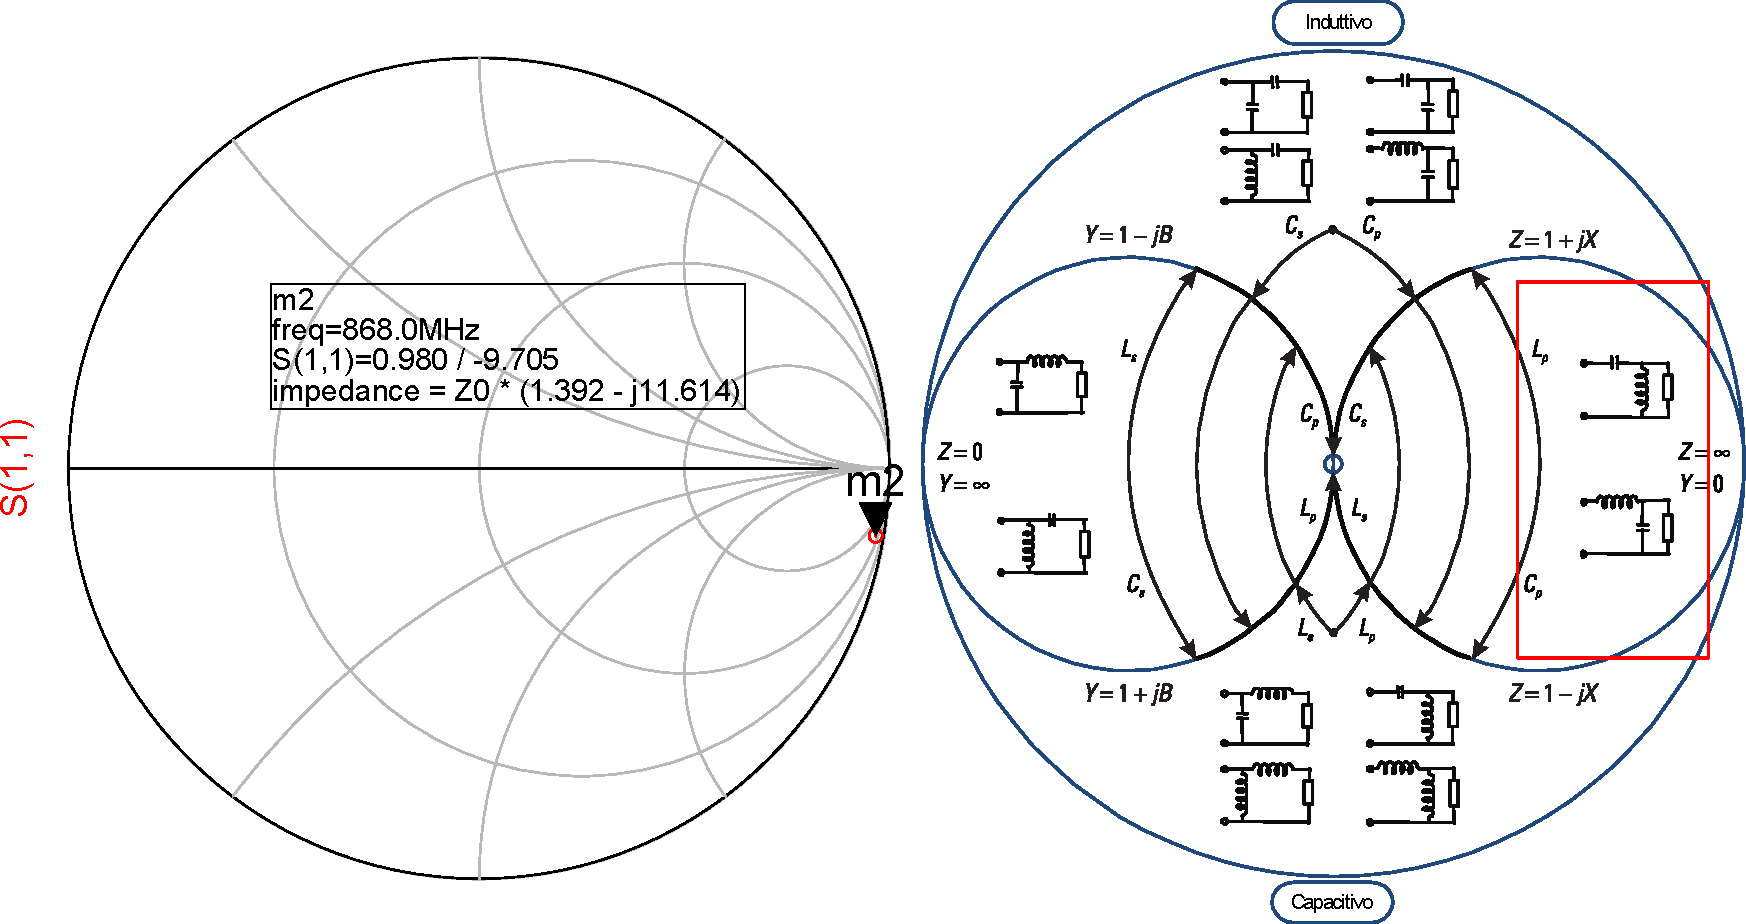
\includegraphics[width=15cm]{AdattImp}
\caption{Impedenza da adattare e possibili reti a L.}
\label{fig:AdattImp}
\end{figure}

\newpage
A questo punto quindi siamo partiti realizzando le reti LC, sfruttando inizialmente componenti ideali (tab. \ref{tab:adatt1}) e poi quelli reali (tab. \ref{tab:adatt2}) forniti dalla librerie Murata precedentemente installate come \itt{add-on}.

\begin{table}[ht!]
\centering
\begin{tabular}{|c|c|c|}
\hline
Rete di adattamento & Valori dei componenti & Soglia di rivelazione \\ \hline % \hline
\begin{tabular}{c} 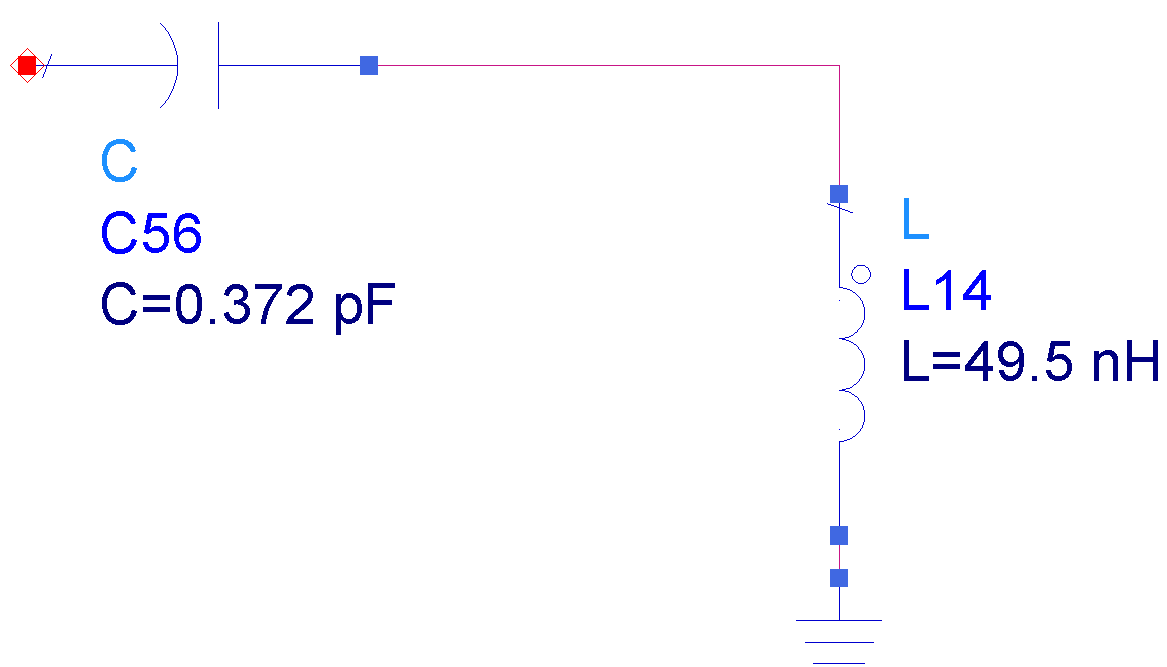
\includegraphics[width=5cm]{LC1id} \\ \end{tabular} &
\begin{tabular}{c} L = 49,5 nH \\ C = 0,372 pF \\ \end{tabular} &
\begin{tabular}{c} -46,99 dBm \\ \end{tabular} \\ \hline
\begin{tabular}{c} 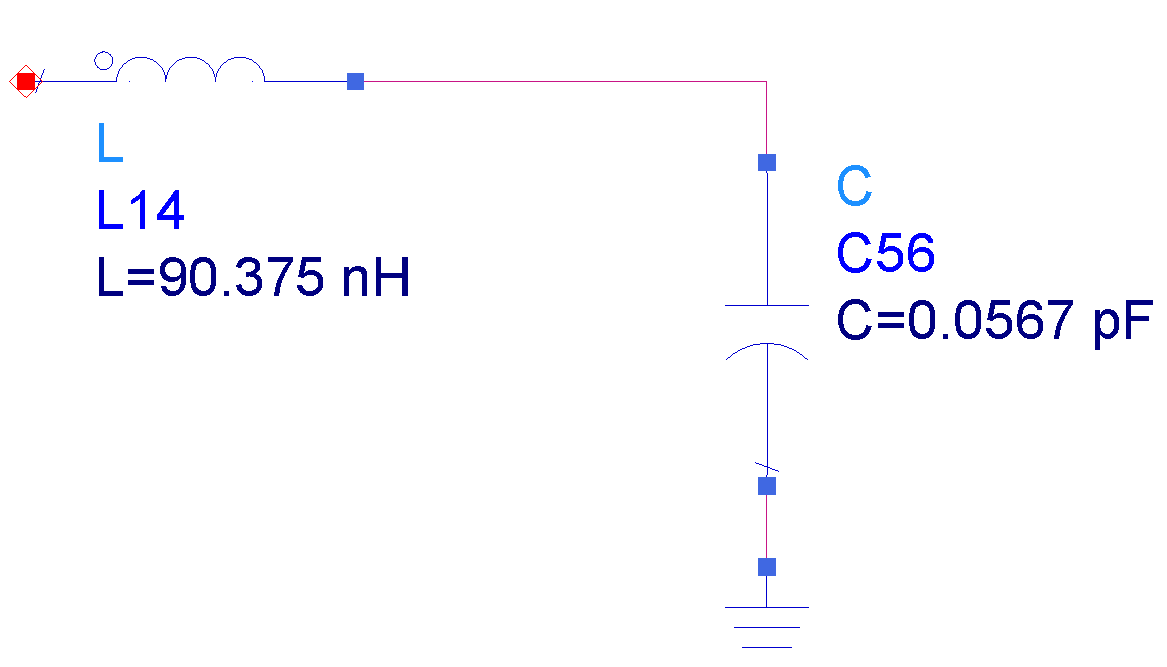
\includegraphics[width=5cm]{LC2id} \\ \end{tabular} &
\begin{tabular}{c} C = 0,0567 pF \\ L = 90,375 nH \\ \end{tabular} &
\begin{tabular}{c} -46,99 dBm \\ \end{tabular} \\ \hline
\end{tabular}
\label{tab:adatt1}
\caption{Reti di adattamento a L con componenti ideali.}
\end{table}


I componenti Murata si basano su modelli matematici (ottenuti per \itt{fitting} su risultati empirici) in grado di tener conto anche del comportamento in frequenza dei componenti parassiti presenti in ogni elemento fisico; per questo motivo i valori trovati risultano diversi da quelli ideali ed anche il punto di adattamento sar� diverso dallo Z = 1 + j0 dei due casi precedenti (per questo viene mostrato il suo valore nella tabella \ref{tab:adatt2}).


\begin{table}[ht!]
\centering
\begin{tabular}{|c|c|c|}
\hline
Rete di adattamento & Valori dei componenti & Soglia di rivelazione \\ \hline % \hline
\begin{tabular}{c} 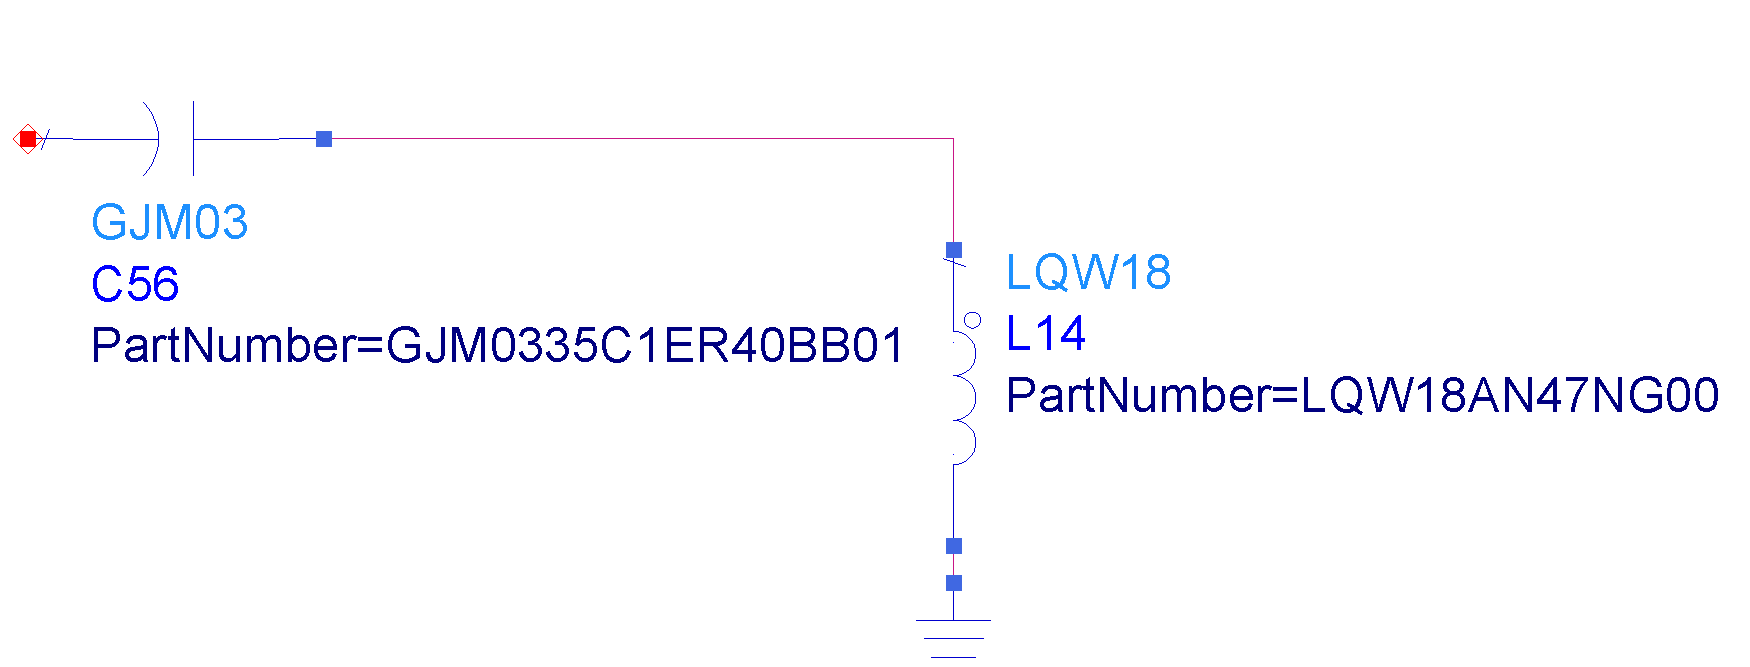
\includegraphics[width=7cm]{LC1re} \\ \end{tabular} &
\begin{tabular}{c} L = 47 nH \\ C = 0,4 pF \\ Z = 1,143 + j0,277 \\ \end{tabular} &
\begin{tabular}{c} -45,89 dBm \\ \end{tabular} \\ \hline
\begin{tabular}{c} \includegraphics[width=7cm]{LC2re} \\ \end{tabular} &
\begin{tabular}{c} C = 0,1 pF \\ L = 75 nH \\ Z = 0,919 - j0,152 \\ \end{tabular} &
\begin{tabular}{c} -46,34 dBm \\ \end{tabular} \\ \hline
\end{tabular}
\label{tab:adatt2}
\caption{Reti di adattamento a L con componenti reali.}
\end{table}

\newpage
Oltre alla rete ad L, abbiamo provato a realizzare anche un
adattamento a singolo componente, con un induttore serie, visto che il valore dell'impedenza da
adattare � molto vicino al cerchio a resistenza costante unitaria. In tabella \ref{tab:adatt3} sono indicati i valori utilizzati
rispettivamente per il caso ideale e reale; in questo caso non raggiungiamo un perfetto
adattamento, ma la soglia di rivelazione � comunque molto vicina al valore limite trovato nei casi
ideali (-46,99 dBm) ed inoltre utilizziamo un singolo componente riducendo lo spazio occupato ed il
costo.

\begin{table}[ht!]
\centering
\begin{tabular}{|c|c|c|}
\hline
Rete di adattamento & Valori dei componenti & Soglia di rivelazione \\ \hline % \hline
\begin{tabular}{c} \includegraphics[width=5cm]{Lid} \\ \end{tabular} &
\begin{tabular}{c} L = 106,5 nH \\ Z = 1,392 + j0,003 \\ \end{tabular} &
\begin{tabular}{c} -46,89 dBm \\ \end{tabular} \\ \hline
\begin{tabular}{c} \includegraphics[width=5cm]{Lre} \\ \end{tabular} &
\begin{tabular}{c} L = 100 nH \\ Z = 1,570 + j0,294  \\ \end{tabular} &
\begin{tabular}{c} -46,19 dBm \\ \end{tabular} \\ \hline
\end{tabular}
\label{tab:adatt3}
\caption{Reti di adattamento a singolo componente.}
\end{table}

Una volta ricavati gli adattamenti a costanti concentrate siamo passati alle linee di trasmissione
ideali (tab. \ref{tab:adatt4}), con degli stub serie e parallelo e due esempi di trasformatori a $\lambda / 4$. I
risultati ottenuti per gli ultimi due casi sono stati quelli pi� interessanti, che ci hanno consentito di
scartare direttamente l'ipotesi di una realizzazione in microstrisce di queste configurazioni ideali a
$\lambda / 4$. Infatti i valori di impedenza che � possibile ottenere fisicamente con le microstrisce variano nel
range tra 20 e 200 $\Omega$ circa. Il limite superiore � dato dalla difficolt� realizzativa, in quanto valori
superiori a 200 $\Omega$ implicano una larghezza di pista troppo piccola tale da enfatizzare gli effetti parassiti per
lo sfrangiamento del campo, mentre valori di impedenza inferiori a 20 $\Omega$ comportano una larghezza molto elevata con notevole diminuzione della frequenza di cut-off dei modi superiori.

\begin{table}[ht!]
\centering
\begin{tabular}{|c|c|c|}
\hline
Rete di adattamento & Valori dei componenti & Soglia di rivelazione \\ \hline % \hline
\begin{tabular}{c} \includegraphics[width=5cm]{TL1} \\ \end{tabular} &
\begin{tabular}{c} TLS \\ Z = 50 $\Omega$ \\ E = 90,89\textdegree \\ $f = 868$ MHz \\ \\ 
TLP \\ Z = 50 $\Omega$ \\ E = 174,2\textdegree \\ $f = 868$ MHz \\ \end{tabular} &
\begin{tabular}{c} -46,99 dBm \\ \end{tabular} \\ \hline

\begin{tabular}{c} \includegraphics[width=5cm]{TL2} \\ \end{tabular} &
\begin{tabular}{c} TLS1 \\ Z = 50 $\Omega$ \\ E = 85,15\textdegree \\ $f = 868$ MHz \\ \\ 
TLS2 \\ Z = 5,03 $\Omega$ \\ E = 90\textdegree \\ $f = 868$ MHz \\ \end{tabular} &
\begin{tabular}{c} -46,99 dBm \\ \end{tabular} \\ \hline

\begin{tabular}{c} \includegraphics[width=5cm]{TL3} \\ \end{tabular} &
\begin{tabular}{c} TLS1 \\ Z = 50 $\Omega$ \\ E = 175,15\textdegree \\ $f = 868$ MHz \\ \\ 
TLS2 \\ Z = 497,6 $\Omega$ \\ E = 90\textdegree \\ $f = 868$ MHz \\ \end{tabular} &
\begin{tabular}{c} -46,99 dBm \\ \end{tabular} \\ \hline

\end{tabular}
\label{tab:adatt4}
\caption{Reti di adattamento con linee ideali.}
\end{table}

Per quanto riguarda il primo caso di adattamenti della tab. \ref{tab:adatt4}, siamo passati alla realizzazione in
microstriscia con un substrato di tipo FR4 (caratteristiche in fig. \ref{fig:MSub}) sfruttando sempre il tool
\itt{LineCalc} e aggiustando poi i valori tramite uno sweep in frequenza, per ottenere i valori della tab. \ref{tab:adatt5}.
%(Vuoi anche un commento sulle lunghezze degli stub rispetto alla lunghezza d�onda a 868 MHz?Commento anche su la soglia di rivelazione non tanto buona rispetto agli altri casi per via delle perdite?)

\begin{figure}[ht!]
\centering % \hspace{2cm}
\includegraphics[width=2.5cm]{MSub}
\caption{Caratterizzazione del substrato.}
\label{fig:MSub}
\end{figure}

\begin{table}[ht!]
\centering
\begin{tabular}{|c|c|c|}
\hline
Rete di adattamento & Valori dei componenti & Soglia di rivelazione \\ \hline % \hline
\begin{tabular}{c} \includegraphics[width=5cm]{ML} \\ \end{tabular} &
\begin{tabular}{c} MLS \\ W = 1503,6 $\mu$m \\ L = 52450 $\mu$m \\ \\ 
MLP \\ W = 1503,6 $\mu$m \\ L = 88380 $\mu$m \\ \end{tabular} &
\begin{tabular}{c} -39.47 dBm \\ \end{tabular} \\ \hline

\end{tabular}
\label{tab:adatt5}
\caption{Reti di adattamento con microstrisce.}
\end{table}

\newpage
Infine abbiamo studiato tre casi di adattamenti ``ibridi'', con microstrisce e componenti Murata (tab. \ref{tab:adatt6}); rispettivamente nel primo esempio un tratto di linea in serie e una rete LC (L serie e C shunt); poi
una versione semplificata con un solo componente concentrato rispetto a prima e per ultimo caso
uno stub in circuito aperto (comprensivo di effetti di sfrangiamento del campo) seguito da una
induttanza serie.

\begin{table}[ht!]
\centering
\begin{tabular}{|c|c|c|}
\hline
Rete di adattamento & Valori dei componenti & Soglia di rivelazione \\ \hline % \hline

\begin{tabular}{c} \includegraphics[width=7cm]{Ib1} \\ \end{tabular} &
\begin{tabular}{c} MLS \\ W = 1500 $\mu$m \\ L = 630 $\mu$m \\ 
\\ L = 82 nH \\ C = 1,1 pF \\ Z = 1,173 - j0,056 \\ \end{tabular} &
\begin{tabular}{c} -46.19 dBm \\ \end{tabular} \\ \hline

\begin{tabular}{c} \includegraphics[width=7cm]{Ib2} \\ \end{tabular} &
\begin{tabular}{c} MLS \\ W = 1500 $\mu$m \\ L = 507 $\mu$m \\ 
\\ L = 82 nH \\ Z = 1,140 - j0,035 \\ \end{tabular} &
\begin{tabular}{c} -46.29 dBm \\ \end{tabular} \\ \hline

\begin{tabular}{c} \includegraphics[width=7cm]{Ib3} \\ \end{tabular} &
\begin{tabular}{c} MLEF \\ W = 1500 $\mu$m \\ L = 240 $\mu$m \\ 
\\ L = 82 nH \\ Z = 1,108 + j0,117 \\ \end{tabular} &
\begin{tabular}{c} -46.29 dBm \\ \end{tabular} \\ \hline

\end{tabular}
\label{tab:adatt6}
\caption{Reti di adattamento ibride.}
\end{table}

Alla fine � stata scelta la rete reale di tab. \ref{tab:adatt3} perch� garantisce un'ottima soglia di rivelazione minimizzando le dimensioni fisiche del circuito. Questa configurazione potrebbe servire come modello per una realizzazione in laboratorio del power detector, vista la disponibilit� di componenti LQW18.

\section{Risposta transitoria}

\par Nell'ultima parte dell'esercitazione siamo andati a studiare il comportamento del circuito, non pi� a regime come nelle simulazioni DC e HB, ma al transitorio per studiare la scarica del condensatore $\mathrm{C}_1$ al variare del suo valore e l'effetto che esso produce sul circuito. Per farlo abbiamo utilizzato un nuovo tipo di simulatore, il \itt{Transient/Convolution}.

\subsubsection*{Simulatore \itt{Transient/Convolution}}

\par Mentre l'analisi attraverso i parametri S, vista nella parte precedente relativa agli adattamenti,
linearizza il circuito e opera nel dominio della frequenza, l'analisi \itt{Transient/Convolution} \cite{TrConv} simula le
performance del circuito nel dominio del tempo. Inoltre include tutte le propriet� non lineari dei
componenti e all'aumentare della complessit� del circuito pu� richiedere una quantit� significativa
di tempo per essere completata e generare un'elevatissima quantit� di dati, come ci � capitato di
verificare nel corso dell'esercitazione.
I simulatori Transient e Convolution sono simili allo SPICE nel loro modo di operare, in quanto vanno
a risolvere un insieme di equazioni integro-differenziali che esprime la dipendenza dal tempo delle
correnti e tensioni del DUT. Il risultato � un'analisi non lineare in funzione del tempo. La differenza
principale tra le opzioni Transient e Convolution si trova nella caratterizzazione degli elementi
distribuiti e dipendenti dalla frequenza presenti nel circuito.

\par L'analisi Transient viene effettuata completamente nel dominio del tempo, e perci� non � in grado di
stimare il comportamento in frequenza di elementi distribuiti come le microstrisce, le linee a striscia, ecc. Quindi tali elementi devono essere rappresentati da modelli semplificati, indipendenti dalla
frequenza come ad esempio elementi a costanti concentrate equivalenti, linee di trasmissione con
perdite ma prive di dispersione, ecc. 

\par L'analisi Convolution invece rappresenta tutti gli elementi distribuiti nel dominio della frequenza e
quindi riesce a studiarne il comportamento al variare della frequenza, molto utile per la
caratterizzazione della maggior parte degli elementi distribuiti a RF e microonde, in quanto non
sempre � possibile ottenere l'esatto equivalente nel dominio del tempo per questi elementi. La
Convolution converte le informazioni nel dominio della frequenza provenienti da tutti gli elementi
distribuiti nel dominio del tempo, ottenendo sostanzialmente la risposta impulsiva di tali elementi. I
segnali di ingresso nel dominio del tempo applicati ai terminali degli elementi vengono convoluti
con la loro risposta impulsiva per ottenere il segnale di uscita (sistema LTI). Gli elementi, anche
non lineari, gi� dotati di precisi modelli equivalenti a costanti concentrate vengono invece
interamente caratterizzati nel dominio del tempo senza bisogno della risposta impulsiva.

\par Il simulatore, una volta impostato il range temporale di interesse, le tolleranze e il limite massimo di
iterazioni, procede con un'analisi DC per determinare le condizioni iniziali.
L'importante � impostare correttamente il parametro \textsf{MinTimeStep}, che dovr� essere inferiore al pi�
veloce tempo di salita (rise time) presente nel circuito.
Intanto all'interno del simulatore viene generata una \itt{table breakpoint} per tenere traccia dei
dispositivi dipendenti dalla frequenza e dei dati accumulati. In particolare la tabella contiene anche
una lista ordinata di tutti i punti di transizione delle sorgenti indipendenti del DUT, che
normalmente non coincidono con il \textsf{TimeStep} calcolato dal programma. In questo modo durante la
simulazione, quando il prossimo punto temporale � abbastanza vicino ad uno dei breakpoint, il
passo temporale viene automaticamente aggiustato per farlo coincidere con quest'ultimo. In seguito il simulatore tenta di risolvere il sistema di equazioni attraverso un'integrazione numerica e un numero finito di iterazioni col metodo \itt{Newton-Rapshon}. Se il numero di iterazioni supera il limite imposto da \textsf{Max Iterations per time point}, allora il \textsf{TimeStep} viene diminuito di un fattore pari al coefficiente di integrazione \textsf{Mu} diviso per 8. A questo punto se il nuovo passo temporale � accettabile si procede oltre, altrimenti in caso di coefficiente di
integrazione pari a zero, viene usato il \itt{Backward-Euler} come metodo numerico di integrazione. In
seguito per la convergenza viene calcolato l'errore locale di troncamento (\textsf{Local Truncation Error},
LTE) con il metodo di integrazione trapezoidale. Nel caso di mancata convergenza per circuiti pi�
complessi � possibile sfruttare anche il metodo di \itt{Gear}. Dalla
stima dell'LTE viene trovato l'intervallo del \textsf{TimeStep} ed in seguito l'errore viene confrontato coi
limiti imposti dalle tolleranze; se l'errore � ammissibile i risultati vengono salvati e l'analisi
continua col punto successivo, altrimenti si ripete tutto il procedimento con un passo pi� piccolo.
Spesso per evitare errori nella simulazione � necessario controllare il comportamento in frequenza
di alcuni componenti (quali induttori, condensatori, ecc.) ed i modelli che sfruttano, talvolta non adatti
alla simulazione in corso. Inoltre per aumentare la velocit� della simulazione e risolvere problemi di
convergenza (a discapito dell'accuratezza, come � stato nel nostro caso), bisogna diminuire, rispetto
ai valori di default, le tolleranze relative e assolute per le correnti e le tensioni, e soprattutto il
parametro \textsf{ChargeTol} per la tolleranza adottata nel calcolo dell'LTE. Infatti ogni aumento
dell'ordine di grandezza porta all'incirca ad un numero di punti temporali triplicato, aumentando
vertiginosamente il tempo totale di simulazione e la quantit� di dati generati.
Il settaggio dei parametri per la nostra simulazione e rappresentato in fig. \ref{fig:Transient}.

\begin{figure}[ht!]
\centering % \hspace{2cm}
\includegraphics[width=4cm]{Transient}
\caption{Impostazione della simulazione Transient.}
\label{fig:Transient}
\end{figure}

Una volta descritta e impostata la simulazione Transient/Convolution, abbiamo
visualizzato (fig. \ref{fig:transientout} ) la risposta transitoria del circuito tra 0 e 100 $\mu$s a -30 dBm (16 dBm sopra la soglia) di potenza erogata dal generatore, e impostando i seguenti valori di capacit� : 10, 32, 100, 320 e 1000 pF. Scegliendo opportunamente il valore di capacit�, si determina la durata minima dell'impulso di potenza, quella corrispondente ad una variazione da livello basso ad alto dell'uscita del comparatore.

\begin{figure}[ht!]
\centering % \hspace{2cm}
\includegraphics[width=12cm]{transientout}
\caption{Risposta del comparatore ad un impulso di -30 dBm al variare della capacit�.}
\label{fig:transientout}
\end{figure}

Come si vede dalla figura \ref{fig:transientC}, all'aumentare del valore di capacit�, la scarica del condensatore diventa pi� lenta, raggiungendo comunque il medesimo valore di tensione a regime al nodo A. Si noti come viene risaltato l'effetto di \itt{feedthrough} (trasudamento) del segnale al diminuire del valore della capacit�. 

\begin{figure}[ht!]
\centering % \hspace{2cm}
\includegraphics[width=16cm]{transientC}
\caption{Scarica del condensatore $\mathrm{C}_1$ per pi� valori di capacit� ed effetto trasudamento.}
\label{fig:transientC}
\end{figure}

\graphicspath{{img/lab3/}}
\chapter{Transceiver FSK in banda ISM a 2.4 GHz}

%\section{Introduzione}

\par In questo capitolo viene presentata l'analisi di un sistema di ricetrasmissione wireless con una modulazione FSK (\textit{Frequency Shift Keying}), in banda ISM a 2.4 GHz. Le ISM (\itt{Industrial Scientific and Medical}) sono bande non licenziate ma regolamentate, originariamente dedicate ad applicazioni industriali, scientifiche e biomedicali che sfruttassero campi elettromagnetici a radiofrequenze per scopi diversi dalle telecomunicazioni. Oggigiorno vengono anche utilizzate da apparati di comunicazione a raggio corto o SRD (\itt{Short Range Devices}) quali il transceiver che verr� progettato. L'obiettivo della simulazione eseguita a livello di sistema per una catena di trasmissione unidirezionale � di ricavarne le prestazioni in termini di probabilit� di errore o BER (\textit{Bit Error Rate}) al variare del rapporto segnale rumore o SNR (\textit{Signal to Noise Ratio}) in ingresso al ricevitore.

\par In una prima parte verr� discussa la modulazione FSK e le sue caratteristiche principali. In seguito verr� presentata l'architettura del transceiver FSK implementata discutendone i blocchi costitutivi. Infine, verr� stimato l'andamento del BER al variare dell'SNR mediante un apposito circuito.

\subsubsection*{Simulatore \textit{Circuit Envelope}}

\par Il simulatore di cui faremo largo impiego nel progetto � il \itt{Circuit Envelope} di ADS \cite{Env}, adeguato per segnali modulati. L'Envelope utilizza l'Harmonic Balance per analizzare le variazioni spettrali di un segnale RF intorno alla sua portante ed alle sue armoniche specificate. In effetti, l'Envelope campiona ad istanti definiti dal progettista l'ampiezza e la fase delle righe spettrali generate da una simulazione Harmonic Balance, e ricostruisce quindi, dai campioni ottenuti dalle variazioni della riga alla frequenza portante, il segnale modulante. Dall'inviluppo complesso del segnale RF cos� dedotto, � possibile, tramite FFT (\itt{Fast Fourier Transform}) estrapolare lo spettro (densit� spettrale di potenza) del segnale RF, con risoluzione frequenziale proporzionale al rapporto tra la frequenza di campionamento e il numero di campioni acquisiti\footnote{$\Delta f = \frac{F_s}{N}$, con $F_s$ frequenza di campionamento e $N$ numero di campioni acquisiti.}. Si possono quindi ottenere dallo spettro generato diversi parametri che caratterizzano le prestazioni del transceiver, quali l'\itt{Adjacent Channel Power Ratio} che fornisce una stima della potenza immessa nei canali adiacenti, il \itt{Noise Power Ratio}, in un sistema a multiplazione di frequenza, indice di ``riposo'' di un canale libero nel quale vengono a cadere prodotti di intermodulazione dei canali adiacenti, e ben altri parametri. Per quanto riguarda il nostro progetto dovremo verificare la conformit� del trasmettitore alle norme europee sulla compatibilit� elettromagnetica in banda ISM, specificate in termini di potenza totale irradiata. Inoltre la valutazione dell'SNR in ingresso al ricevitore verr� eseguita mediante integrazione dello spettro intorno alla portante.

\section{Modulazione FSK}

\par La modulazione FSK � una modulazione digitale che, come l'FM (\textit{Frequency Modulation}) in analogico, consiste nel far variare la frequenza della portante in proporzione al segnale modulante. Il segnale modulante, essendo digitale e quindi caratterizzato da due livelli discreti, sar� tale da produrre variazioni pressoch� istantanee della frequenza della portante come illustrato in figura \ref{fig:timefsk}.
\begin{figure}[ht!]
\centering
\includegraphics[width=8cm]{fsk}
\caption{Modulazione FSK e andamento temporale dei segnali.}
\label{fig:timefsk}
\end{figure} Il segnale modulante � binario e un singolo bit rappresenta un tono in frequenza: questa modulazione viene detta \textit{Binary-FSK} (BFSK) ed � proprio il tipo di modulazione che verr� implementata. La modalit� di sintesi del segnale RF di figura \ref{fig:timefsk}, che presenta una variazione di fase continua viene chiamata \textit{Continuous Phase FSK} o CPFSK\footnote{Come vedremo nel paragrafo \ref{sect:tx} questa si ottiene mediante un \textit{Voltage Controlled Oscillator}.\label{fn:VCOFSK}}. Essa si contrappone alla sintesi di due toni scorrelati commutati a seconda del livello del segnale modulante. Utilizzando pi� di una portante, si pu� estendere la BFSK ad una \textit{M-ary FSK}, aumentando cos� il \textit{throughput} dei dati. Questa soluzione � particolarmente complessa e spettralmente inefficiente. Si preferisce quindi, per aumentare il numero di bits per simbolo, utilizzare modulazioni M-PSK (\textit{M-ary Phase Shift Keying}) oppure ibride in ampiezza e fase quali le QAM (\textit{Quadrature Amplitude Modulation}) \cite{Haykin}.

%\subsection{Specifiche di progetto}

\par Vediamo in dettaglio le specifiche di modulazione del transceiver da progettare. Il segnale modulante � un \textit{bitstream} di 40 kbps. La portante � fissata a $f_{LO} = 2,44$ GHz. La deviazione di frequenza $\Delta f$ � stata scelta di 50 kHz, ottenendo cosi le frequenze $f_\mathit{space} = f_{LO} - \Delta f$ per il bit 0 e $f_\mathit{mark} = f_{LO} + \Delta f$ per il bit 1. L'indice di modulazione FSK � quindi di $\frac{2 \cdot 50 \mathrm{kHz}}{40 \mathrm{kpbs}} = 250$\%, largamente maggiore del 50\% necessario per una corretta demodulazione. Nella seguente figura \ref{fig:spettrofsk} viene illustrato lo spettro, evidenziando l'andamento tipico di una modulazione BFSK.
\begin{figure}[ht!]
\centering
\includegraphics[width=11cm]{spettro}
\caption{Spettro della modulazione FSK da implementare.}
\label{fig:spettrofsk}
\end{figure} La natura digitale del \textit{bitstream} fa s� che lo spettro complessivo sia dato da due \textsf{sinc} ($\mathrm{sinc(\mathit{f})} = \frac{\sin(\pi f)}{\pi f}$) con lobi principali larghi 80 kHz posti intorno alla frequenza portante ad una distanza proporzionale all'indice di modulazione.
\par Il segnale in banda base � di tipo NRZ (\textit{Non Return to Zero}) e il 99\% della potenza � confinata entro $f_\mathrm{BB} = \frac{9,5}{T_b}$ dove $T_b$ � il tempo di bit che in tal caso � di $\frac{1}{40000} \mathrm{{Hz}^{-1}} = 25 \ {\mu}s$ \cite{Anderson}. Questo si traduce in una banda $f_\mathrm{BB}$ di 380 kHz, valore eccessivo per un sistema di ricetrasmissione RF a banda limitata (in rispondenza ad uno standard che limiti la larghezza dei canali e la potenza immessa nei canali adiacenti). Per effetto dell'\textit{upconversion} la banda a RF $f_\mathrm{RF}$ diverrebbe di $2 \cdot f_\mathrm{BB} = 760$ kHz per il solo tono di \textit{space} o \textit{mark}. Va quindi aggiunto lo scarto di 100 kHz per arrivare ad un valore complessivo di 860 kHz, traducendosi in un efficenza spettrale di soli $\frac{40 \mathrm{kbps}}{860 \mathrm{kHz}} \approx 5 \%$. Si ricorre quindi a tecniche di \textit{pulse shaping} mediante particolari filtraggi, ad esempio un filtro \textit{raised cosine}\footnote{I filtri \textit{raised cosine}, oltre a restringere la banda, minimizzano l'interferenza intersimbolica o ISI \cite{Razavi}.} (coseno rialzato) in modo che la banda utile (99\% della potenza) risulti di un valore adeguato ad una tecnica di modulazione FDM (\textit{Frequency Division Multiplexing}). Si pu� anche intuire che una compressione spettrale di un segnale presenta notevoli vantaggi nei confronti del rumore bianco AWGN (\textit{Additive White Gaussian Noise}) in ingresso al ricevitore, rumore che pu� essere ridotto mediante un filtraggio passa banda pi� stretto.

\section{Architettura del transceiver}

\par Vediamo adesso come � stato scelto di progettare il sistema di ricetrasmissione e quindi di valutarne le prestazione. Lo schema di simulazione viene illustrato in figura \ref{fig:schemasim}.
\begin{figure}[ht!]
\centering
\includegraphics[width=16cm]{schema}
\caption{Schema di simulazione del transceiver FSK.}
\label{fig:schemasim}
\end{figure} Un \itt{bitstream} modulato e traslato a radiofrequenze viene irradiato da un'antenna isotropica. La propagazione avviene in campo aperto in presenza del terreno. L'attenuazione geometrica e quella per riflessione sul terreno verranno considerate nel canale di trasmissione mediante un opportuna equazione dipendente dalla distanza relativa e l'altezza dal suolo delle antenne coinvolte. Immediatamente prima dell'antenna ricevente, anche essa di guadagno unitario, viene aggiunto al segnale captato rumore termico a 300~K (temperatura ambiente di circa 27 \textdegree{C}). Il \itt{font end} del ricevitore vedr� quindi un determinato SNR al variare della distanza, valore che influenzer� la corretta rivelazione del \itt{bitstream}. Il BER verr� misurato confrontando i \itt{bitstream}, quello ricevuto con quello trasmesso traslato del ritardo di propagazione tra i blocchi della catena di comunicazione. Uno sweep sulla distanza ci permetter� di ricostruire l'andamento del BER al variare dell'SNR.

\subsection{Trasmettitore}\label{sect:tx}

\par Il trasmettitore FSK esegue una conversione diretta a $f_\mathrm{RF}$ mediante un VCO (\textit{Voltage Controlled Oscillator}) che sintetizza un segnale RF con variazioni di fase continue\footnote{Questa tecnica di modulazione CPFSK si contrappone alla sintesi mediante due oscillatori a $f_\mathrm{space}$ e $f_\mathrm{mark}$ commutati dal segnale modulante. In questo caso il segnale RF sintetizzato presenta variazioni istantanee di fase che si ripercuotono sullo spettro allargandone la banda.}. In figura \ref{fig:tx} viene illustrato lo schema a blocchi del trasmettitore.
\begin{figure}[ht!]
\centering
\includegraphics[width=16cm]{tx}
\caption{Schema a blocchi del trasmettitore.}
\label{fig:tx}
\end{figure} Un generatore di treno d'impulsi pseudo-random sintetizza un bitstream NRZ di 40 kbps, con livelli di tensione bilanciati di 1 V. Il segnale cos� generato viene filtrato da un passa basso \textit{raised cosine} RC, che presenta una risposta impulsiva della forma \cite{Razavi}:
\begin{equation}
\label{eq:raisedcosine}
p(t) = \mathrm{sinc} \left ( \frac{t}{T_b} \right ) \cdot \frac{\cos(\frac{\pi \alpha t}{T_b})}{1 - \frac{4 \alpha^2 t^2}{{T_b}^2}}
\end{equation} dove $T_b$ � il tempo di bit e il coefficiente $\alpha$ � compreso tra 0 e 1 e viene detto fattore di \itt{rolloff}. In effetti, al crescere di $\alpha$ si ha un decadimento maggiore delle code del \textsf{sinc} della risposta impulsiva del filtro. Da un punto di vista spettrale, un aumento di $\alpha$ implica, scostandosi da 0, per cui si ha una finestra rettangolare, una minor ripidit� in banda di transizione del filtro passa basso. Per questo motivo il fattore $\alpha$ viene anche chiamato \itt{eccesso di banda} e valori tipicamente utilizzati sono compresi tra 30\% e 40\% \cite{Anderson}. Nel nostro caso si � scelto un $\alpha$ di 35\% con una frequenza equivalente di bitstream raddoppiata ($f_\mathrm{equiv} = 80 \mathrm{kHz}$). La banda del filtro diventa quindi di $f_\mathrm{LPF} = \frac{(1+\alpha)}{2 T_\mathrm{equiv}} \approx 54 \mathrm{kHz}$. Lo spettro che si ottiene prima e dopo il filtraggio � illustrato in figura \ref{fig:TxRx_baseband}, illustrando il {rolloff} dello spettro del segnale filtrato con conseguente restringimento della banda utile.
\begin{figure}[ht!]
\centering
\includegraphics[width=9cm]{TxRxbaseband}
\caption{Spettro del bitstream in banda base, prima e dopo il filtraggio RC.}
\label{fig:TxRx_baseband}
\end{figure}

\par Il blocco successivo del trasmettitore � il VCO. Esso � centrato a 2,44 GHz e presenta una sensibilit� di 50 kHz/V in modo da ottenere la deviazione di frequenza di progetto (Figura \ref{fig:spettrofsk}). La potenza del segnale RF � di -10 dBm.

\par Al VCO seguono un'amplificatore di potenza PA e un filtro passa banda Chebyshev tale da attenuare le armoniche della portante. Sia il VCO che il PA presentano non linearit� tali da generare componenti spurie fuori banda non trascurabili.

\par Per rispettare la direttiva europea 2004/108/EC sulla compatibilit� elettromagnetica per SRD generici \cite{ERCREC}, � necessario che la potenza irradiata non superi un EIRP (\itt{Effective Isotropic Radiated Power}) di 10 dBm. L'EIRP � la potenza irradiata da un trasmettitore di riferimento provvisto di un'antenna isotropica tale da produrre il medesimo campo del trasmettitore considerato nella sua direzione di massima guadagno. Per il trasmettitore progettato � stato considerato l'impiego di un'antenna isotropica (antenna ideale di guadagno unitario). L'utilizzo di un'antenna reale significa sottoscalare il guadagno del PA di un valore pari al guadagno d'antenna\footnote{Con un dipolo, il guadagno di 2,15 dB verrebbe ad abassare la soglia specificata dalla norma a 7,85 dBm.}. Nella seguente figura si illustrano gli spettri dei segnali prima del PA e ai morsetti dell'antenna isotropica. Viene inoltre raffigurato lo spettro irradiato alla seconda armonica.
\begin{figure}[ht!]
\centering
\includegraphics[width=15cm]{TxRxradiated}
\caption{Spettro in trasmissione e valutazione dell'EIRP.}
\label{fig:TxRx_radiated}
\end{figure}

\par Per integrare lo spettro � stata utilizzata la funzione \textsf{spec{\textunderscore}power(PSD, $f_\mathrm{min}$, $f_\mathrm{max}$)}, che prende in ingresso un array di valori in dBm/Hz di densit� spettrale di potenza (PSD) e integrando nel range specificato restituisce la potenza in dBm. \`E stato applicato ai dati PSD in ingresso un filtraggio Kaiser all'FFT in modo da escludere un eventuale corruzione dell'informazione da campionamento incoerente da parte del simulatore Envelope. Il filtraggio digitale comporta un guadagno da prendere in considerazione nella valutazione della potenza, sottraendolo al valore restituito da \textsf{spec{\textunderscore}power}(). Il filtraggio Kaiser presenta un \itt{Normalized Equivalent Noise BandWidth} di 1,653\footnote{Valori del NENBW per varie finestre di pesaggio sono tabulati in corrispondenza della descrizione della funzione \href{http://edocs.soco.agilent.com/display/ads2009/spectrum+analyzer()}{\textsf{spectrum{\textunderscore}analyzer}()}.} \cite{MeasExp}, ossia un incremento di circa 2,18 dB rispetto ad una finestratura rettangolare (assenza di filtraggio). Come si pu� vedere in figura \ref{fig:TxRx_radiated}, il valore di $\mathsf{WindowGain} = 10 \ {\log}_{10}(1,653) \approx 2,18$dB viene sottratto alla potenza restituita dalla funzione di integrazione. Il valore di 9,982 dBm di EIRP viene raggiunto con un guadagno di PA di 20 dB.

\subsection{Canale di comunicazione e rumore additivo}

\par In questo paragrafo viene trattata, in primo luogo, la propagazione dell'onda elettromagnetica generata considerando come ambiente il campo aperto, ed in seguito, il rumore termico additivo intrinseco ai dispositivi elettronici dell'apparato ricevente. In figura \ref{fig:channelnoise} sono illustrati i blocchi che hanno permesso di implementare questa parte del sistema di ricetrasmissione.
\begin{figure}[ht!]
\centering
\includegraphics[width=11cm]{channelnoise}
\caption{Blocchi di modellizzazione della propagazione e del rumore termico.}
\label{fig:channelnoise}
\end{figure}

\subsubsection{Propagazione in campo aperto}

\par La propagazione del segnale irradiato � stata considerata in campo aperto (\itt{Open Field}), ossia includendo alla propagazione nello spazio libero gli effetti del terreno. Questa situazione � schematizzata in figura \ref{fig:path}.
\begin{figure}[ht!]
\centering
\includegraphics[width=10cm]{path}
\caption{Propagazione in campo aperto.}
\label{fig:path}
\end{figure} La propagazione � data da un cammino diretto $R_1$ ed uno riflesso sulla superficie del terreno $R_2$. L'analisi \cite{Dunlop} dello sfasamento tra le due onde che giungono al ricevitore permette di modellare le perdite di propagazione in campo aperto con la seguente equazione
\begin{equation}
L_\mathrm{OF} = - 10 \ {\log}_{10} \left ( \frac{h_t \cdot h_r}{R^2} \right )^2 \ \ [\mathrm{dB}]
\end{equation} Nel caso in cui l'altezza dell'antenna in trasmissione $h_t$ sia la stessa di quella in ricezione $h_r$ l'equazione \ref{eq:losses} si riduce a
\begin{equation}
\label{eq:losses}
L_\mathrm{OF} = - 40 \ {\log}_{10} \left ( \frac{h_r}{R} \right ) \ \ [\mathrm{dB}]
\end{equation} Nel blocco di attenuazione di figura \ref{fig:channelnoise}, le perdite \textsf{Channel{\textunderscore}Loss} sono modellate con l'equazione \ref{eq:losses} e, per correggere l'entit� delle perdite da quelle ulteriormente introdotte dallo \itt{splitter} a valle impiegato come combinatore, all'equazione vengono sottratti 3 dB. L'altezza � stata arbitrariamente impostata ad 1 m.

\subsubsection{Rumore termico additivo}

\par La densit� spettrale di potenza di rumore termico in ingresso al ricevitore posto ad una temperatura T in Kelvin � $\mathrm{N}_\mathrm{DSP} = \mathrm{kT}$ dove $\mathrm{k} = 1,38 \cdot 10^{-23} \ [{\mathrm{J}}/{\mathrm{K}}]$ � la costante di Boltzmann. A 300 K (27{\textdegree}C), $\mathrm{N}_\mathrm{DSP}$ � di circa -174 dBm. Il generatore di rumore bianco di figura \ref{fig:channelnoise}, impostando opportunamente la tensione \textsf{V{\textunderscore}Noise}, dovr� presentare tale valore a valle dello splitter. 

\par \textsf{V{\textunderscore}Noise} pu� essere determinata analiticamente mediante la formula \textsf{V{\textunderscore}Noise} $= \sqrt{4\mathrm{kTR}}$ \ [V/$\sqrt{\mathrm{Hz}}$] dove R � resistenza di uscita del generatore adattata allo splitter, quindi di 50 $\Omega$. Si ottiene quindi il valore di 910 pV/$\sqrt{\mathrm{Hz}}$, valore che dovr� essere incrementato di un fattore $\sqrt{2}$ per compensare l'attenuazione di 3 dB introdotta dallo splitter. Il valore da impostare � quindi di 1287 pV/$\sqrt{\mathrm{Hz}}$.

\begin{figure}[ht!]
\centering
\includegraphics[width=12cm]{NoiseCalcSchem}
\caption{Schema per la valutazione di \textsf{V{\textunderscore}Noise} mediante il simulatore Envelope.}
\label{fig:NoiseCalcSchem}
\end{figure} 
\par Una strada alternativa a quella analitica � quella di sfruttare la funzione \textsf{spec{\textunderscore}power}() nel circuito di figura \ref{fig:NoiseCalcSchem} valutando la potenza di rumore $\mathrm{P}_\mathrm{n}$ a valle dello splitter. A $\mathrm{P}_\mathrm{n}$ � sufficiente sottrarre il guadagno di integrazione, dato da $10 \ {\log}_{10} \left ( f_\mathrm{max}-f_\mathrm{min} \right )$ per dedurre la densit� spettrale di potenza di rumore $\mathrm{N}_\mathrm{DSP}$. In figura \ref{fig:NoiseCalc_3dBIL} � illustrato lo spettro del rumore generato da una sorgente di 1250 pV/$\sqrt{\mathrm{Hz}}$ e affiancato ad esso una tabella ottenuta per diversi valori di \textsf{V{\textunderscore}Noise}.
\begin{figure}[ht!]
\centering
\includegraphics[width=14cm]{NoiseCalc3dBIL}
\caption{Spettro del rumore a valle dello splitter per \textsf{V{\textunderscore}Noise} = 1250 pV/$\sqrt{\mathrm{Hz}}$ e valori di $\mathrm{N}_\mathrm{DSP}$ per uno sweep di \textsf{V{\textunderscore}Noise} da 600 a 1400 pV/$\sqrt{\mathrm{Hz}}$.}
\label{fig:NoiseCalc_3dBIL}
\end{figure}

%\newpage
\subsection{Ricevitore}

\par Il ricevitore FSK implementato � analogo a quello che veniva utilizzato per i cercapersone (\itt{pagers}) del decennio scorso, dispositivi che hanno riscontrato un notevole interesse per la semplicit� d'impiego ed il basso costo dell'infrastruttura.
\begin{figure}[ht!]
\centering
\includegraphics[width=15cm]{Patent}
\caption{Schema del ricevitore proposto da Ian A. W. Vance.}
\label{fig:Pager}
\end{figure}
Lo schema illustrato in figura \ref{fig:Pager}, tratto da \cite{Vance}, � stato adattato alla nostra modulazione. Si tratta di un integrato in grado di effetuare una demodulazione FSK coerente, utilizzando la componente in fase come dati e quella in quadratura come clock di campionamento di un flip-flop per ricostruire il bitstream trasmesso. Vediamo in dettaglio lo schema a blocchi di figura \ref{fig:rx} che � stato implementato in ADS.
\begin{figure}[ht!]
\centering
\includegraphics[width=17cm]{rx}
\caption{Schema a blocchi del ricevitore.}
\label{fig:rx}
\end{figure} Il segnale captato dall'antenna isotropica del ricevitore viene amplificato da un LNA che presenta un'alta cifra di rumore $\mathrm{NF}_\marm{LNA}$ pari a 8 dB. Valori tipici di NF per LNA sono di 1 - 3 dB \cite{Razavi} e porre $\mathrm{NF}_\marm{LNA}$ ad un tale valore � giustificato dal fatto che i blocchi a valle sono considerati ideali, con NF = 0 dB. $\mathrm{NF}_\marm{LNA}$ diventa quindi la cifra di rumore dell'intero sistema\footnote{A titolo di esempio, un transceiver commerciale quale il CC2500 della Texas Instruments presenta un \itt{overall noise figure} di 16 dB.}. In figura \ref{fig:TxRxreceived} viene mostrato lo spettro del segnale ricevuto, prima e dopo l'amplificatore LNA. Un quantitativo non trascurabile di rumore � stato introdotto dal LNA: � possibile distinguere uno scarto maggiore tra i due spettri fuori dalla banda del segnale, laddove vi � prevalentemente rumore bianco.
\begin{figure}[ht!]
\centering
\includegraphics[width=10cm]{TxRxreceived}
\caption{Spettro captato e quello amplificato dal LNA.}
\label{fig:TxRxreceived}
\end{figure} Il guadagno del LNA � stato impostato a 13 dB. La catena di demodulazione prosegue con uno splitter a 3 dB, di cui una delle due porte di uscita viene seguita da uno sfasatore di 90\textdegree, in modo da ottenere le componenti in quadratura del segnale RF. Nel ricevitore di Vance (figura \ref{fig:Pager}), questi segnali (sfasati di 90\textdegree) si ottengono mediante un ibrido a 90\textdegree \ esterno al chip. I segnali di egual ampiezza cos� sfasati vengono quindi traslati in banda base da due mixer identici nei quali viene immesso il segnale di battimento a $f_\mathrm{LO} = f_\mathrm{RF}$ di 0 dBm. Seguono dei filtri bassa basso tali da attenuare fortemente il \itt{feedthrough} a $f_\mathrm{RF}$ e armoniche e permettere una forte amplificazione (40 dB) del solo segnale utile in banda base. Le componenti in fase I e in quadratura Q vengono ulteriormente amplificate e squadrate, e, avendo assunto una forma digitale, finiscono in ingresso ad un campionatore (\itt{Sample-and-Hold}), la prima come clock e la seconda come dati campionati. In questa fase della demodulazione interessano solamente i punti di attraversamento dello zero ai quali il campionatore � sensibile. Rispetto al ricevitore di Vance (figura \ref{fig:Pager}) i due segnali sono invertiti, ma ci� non compromette la rivelazione in quanto le componenti I e Q contengono la medesima informazione. In uscita del campionatore vi � il bitstream demodulato, idealmente privo di errori in assenza di rumore. I segnali I, Q e il bitstream sono illustrati in figura \ref{fig:TxRxdetected}.
\begin{figure}[ht!]
\centering
\includegraphics[width=10cm]{TxRxdetected}
\caption{Segnali I e Q in banda base e bitstream rilevato per una distanza R di 40m.}
\label{fig:TxRxdetected}
\end{figure}

\section{Prestazioni del transceiver}

\par Vogliamo adesso valutare le prestazioni del ricevitore, essendo la presenza di rumore tale da limitare la capacit� di rivelazione del segnale ricevuto. In particolare, la simulazione verr� eseguita facendo aumentare la distanza relativa R tra trasmettitore e ricevitore in modo da ridurre il livello di segnale captato e quindi l'SNR riscontrato all'antenna del ricevitore. 
\par Le prestazioni vengono tradotte in termini di BER valutato mediante il circuito di figura \ref{fig:BER}. Lo schema di demodulazione scelto fa s� che il bitstream ricevuto sia soggetto a \itt{jitter}. \`E quindi necessario effettuare un campionamento del bitsream ricevuto con un clock di 40 kHz, con fase iniziale opportuna, per ottenere una forma d'onda con tempo di bit costante identico a quello del bitstream trasmesso ($T_b = 25 \ {\mu}s$). Inoltre, per confrontare il bitstream cos� ottenuto con quello trasmesso � necessario traslare il segnale prodotto dal generatore di bitstream in trasmissione di un tempo pari al ritardo introdotto dai blocchi che costituiscono la catena di ricetrasmissione. Una cella di ritardo $\tau$ verr� impostata in modo che avvenga il sincronismo. La fase iniziale del clock e il ritardo $\tau$ verranno determinati graficamente, visualizzando le forme d'onda da sincronizzare.
\begin{figure}[ht!]
\centering
\includegraphics[width=16cm]{BER}
\caption{Schema a blocchi del contatore di errori.}
\label{fig:BER}
\end{figure}
Una volta sincronizzati, i bitstream vengono sottratti mediante lo sfasamento di 180\textdegree \ del bitstream in trasmissione ritardato e combinando con uno splitter i due segnali. Ne risulta un azzeramento in uscita al combinatore soltanto qualora la rivelazione sia priva di errori, ed ogni bit errato viene rilevato da uno dei due contatori a valle, il primo qualora venga ricevuto un bit alto al posto di uno basso e viceversa per il secondo.

\par Procediamo con la sincronizzazione dei bitstream, che verr� eseguita per un trasmettitore posto a 40 m dal ricevitore. 
\begin{figure}[ht!]
\centering
\includegraphics[width=14cm]{BERjitter}
\caption{Jitter sul segnale demodulato.}
\label{fig:BERjitter}
\end{figure}
In figura \ref{fig:BERjitter} si pu� notare il jitter sul segnale ricevuto, confrontandolo con quello trasmesso. Per cancellarlo si eseguir� un campionamento del bitstream ricevuto nei punti centrali dei bits, massimizzando cos� il margine all'errore.
\begin{figure}[ht!]
\centering
\includegraphics[width=13cm]{BERsetupdeltaview}
\caption{Segnali prima della sincronizzazione : $\tau$ e fase iniziale del clock di sincronismo nulli.}
\label{fig:BERsetupdeltaview}
\end{figure}
La figura \ref{fig:BERsetupdeltaview} illustra le forme d'onda dei segnali da confrontare, ossia il bitstream in trasmissione e quello ricevuto campionato, e il clock di campionamento del bitstream ricevuto. \`E stato evidenziato il ritardo netto tra le forme d'onda di $28,75 \ {\mu}s$ ritardo che verr� compensato dalla cella $\tau$.

\begin{figure}[ht!]
\centering
\includegraphics[width=13cm]{BERerratosincronismo}
\caption{Segnali in ingresso allo splitter in assenza di sincronismo.}
\label{fig:BERerratosincronismo}
\end{figure}

\par I segnali in ingresso allo splitter di somma in controfase sono illustrati in figura \ref{fig:BERerratosincronismo}. In assenza di sincronismo, il risultato in uscita dallo splitter � dato dalla somma di due livelli identici, raddoppiando quindi il livello. Il livello risultante � tale da superare la soglia di uno dei contatori che � stata impostata a {0,3~V}. Qualora i bit siano rilevati correttamente, la soglia di {0,3~V} risulta sufficientemente alta da rendere impercettibile ai contatori il rumore in uscita allo splitter di somma.

\par La fase del clock di campionamento � stata ritardata di 90\textdegree, ovvero di $6,25 \ {\mu}s$, in modo che il fronte di salita centri il bit affetto da jitter. Il ritardo $\tau$ � stato quindi posto a $28,75 + 6,25 = 35 \ {\mu}s$. In figura \ref{fig:BERsetupcorrected} si mostrano i risultati di una tale configurazione, accertandone l'assenza di errori quindi il corretto funzionamento.
\begin{figure}[ht!]
\centering
\includegraphics[width=12cm]{BERsetupcorrected}
\caption{Segnali per la misura del BER a sincronismo raggiunto tra bitstream trasmesso e quello ricevuto.}
\label{fig:BERsetupcorrected}
\end{figure}

%\newpage
\subsection{BER vs SNR}

\par Possiamo adesso eseguire uno sweep sulla distanza per ottenere molteplici valori di SNR, ai quali verranno associati i corrispondenti valori di BER. Lo sweep � stato impostato da 40 a 800 m con passi di 40 m. L'SNR viene calcolato con l'ausilio di \textsf{spec{\textunderscore}power()}, integrando in primo luogo lo spettro del segnale attenuato \textsf{SignalPower} (figura \ref{fig:channelnoise}) su $f_\mathrm{RF}$ $\pm 400$ kHz e sottraendone 3 dB per dedurre la potenza di segnale $\mathrm{P}_\mathrm{s}$ a valle dello splitter combinatore. L'integrazione si poteva effettuare entro $\pm 140$ kHz, porzione di spettro contenente la maggior parte della potenza di segnale ($\approx 98\%$) che pu� essere valutata mediante la \itt{formula di Carson} $\mathrm{B}_\mathrm{T} = 2 \ ( 2 \ \Delta f + 1 / T_b)$ \cite{Razavi}. In secondo luogo, l'integrazione dello spettro generato dalla sorgente di rumore \textsf{NoisePower}, scalata di 3 dB per lo stesso motivo precedente, ci permette di ricavare la potenza di rumore $\mathrm{P}_\mathrm{n}$. Entrambe le integrazioni sono eseguite su un medesimo numero di punti frequenziali, quelli per un range di 800 kHz, in modo che le potenze valutate siano proporzionate equamente. Essendo $\mathrm{P}_\mathrm{s}$ e $\mathrm{P}_\mathrm{n}$ valori in dBm, l'SNR si ricava dalla differenza $\mathrm{P}_\mathrm{s} - \mathrm{P}_\mathrm{n}$. Il BER si ottiene dal rapporto tra il numero di bit errati rilevati dai contatori e il numero di bit trasmessi. \`E stato scelto come riferimento per una corretta comunicazione un BER di 0,1\%, implicando la necessit� di trasmettere almeno 1000 bits per raggiungere una precisione di $\nicefrac{1}{1000}$. Il generatore di bitstream (figura \ref{fig:tx}) � stato impostato in modo da produrre 1000 bits, sufficienti per una valutazione qualitativa dell'andamento del BER rispetto all'SNR con un lieve impegno computazionale. In figura \ref{fig:BERsimresults} vengono tabulati i risultati della simulazione. Segue un grafico (fig. \ref{fig:vsR}) che illustra gli andamenti del BER e dell'SNR al variare della distanza.
\begin{figure}[ht!]
\centering
\includegraphics[width=16cm]{BERsimresults}
\caption{Risultati della simulazione per la valutazione di BER e SNR al variare della distanza.}
\label{fig:BERsimresults}
\end{figure} Si noti che oltre i 280 m di distanza relativa tra ricevitore e trasmettitore il BER supera il valore di riferimento di $\leq 10^{-3}$, distanza alla quale l'SNR percepito � di circa 24,5 dB.

\begin{figure}[ht!]
\centering
\includegraphics[width=10cm]{vsR}
\caption{Grafici degli andamenti del BER e dell'SNR al variare della distanza.}
\label{fig:vsR}
\end{figure}


% A questo punto possiamo determinare la sensibilit� $S_i$ (\itt{Minimum Detectable Signal} o MDS) del ricevitore con l'equazione \cite{Razavi}
%\begin{equation}
%\label{eq:sensitivity}
%S_i = - 174 + 10 \ {\log}_{10} \left ( \mathrm{B}_\mathrm{T} \right ) + NF + \mathrm{SNR}_\mathrm{MDS} \ \ \ \ [\mathrm{dBm}],
%\end{equation} e considerando un canale $\mathrm{B}_\mathrm{T}$ di 800 kHz. Si ricava quindi il valore di $S_i = - 174 + 59 + 8 + 24 = -83 \ \mathrm{dBm}$ per un \itt{bitrate} di 40 kbps e un BER di $\leqslant 10^{-3}$. Si noti che questo valore � circa 5 dB al disopra di quello tabulato in fig. \ref{fig:BERsimresults} per R = 280 m.

\par Dai risultati ottenuti � possibile costruire il grafico del BER rispetto all'SNR come quello presentato in figura \ref{fig:BERavgbervssnr}. I 20 punti ricavati dalla simulazione sono stati interpolati linearmente mediante la funzione \textsf{interpolate()}, ottenendo cos� un andamento smussato della curva BER vs SNR, in particolare per valori di SNR alti per i quali viene calcolato un BER nullo, l'accuratezza di 1 bit su 1000 non essendo pi� sufficiente. Viene inoltre evidenziata una curva che approssima l'andamento di tale curva.
\begin{figure}[ht!]
\centering
\includegraphics[width=12cm]{BERavgbervssnr}
\caption{BER vs SNR per una modulazione FSK a 40 kbps.}
\label{fig:BERavgbervssnr}
\end{figure}
%\begin{figure}[ht!]
%\centering
%\includegraphics[width=15cm]{equation}
%\caption{equation.}
%\label{fig:equation}
%\end{figure}


\thispagestyle{myheadings}
\renewcommand\thefigure{\arabic{figure}}
\markright{CONCLUSIONE}
\pagestyle{myheadings}
\phantomsection
\addcontentsline{toc}{chapter}{Conclusione}
\chapter*{Conclusione}


\par I passi avanti della tecnologia, come le tecniche di realizzazione sempre pi� efficienti e rapide, unite
alla ricerche di mercato mirate, hanno portato alla creazione di prodotti - in particolare
nell'elettronica di consumo - che possono essere definiti di ``massa'', nel vero senso della parola.
L'elettronica infatti, dai cellulari, ai personal computer fino alle videocamere, viene prodotta in
quantit� industriale e questo ha reso possibile anche l'abbattimento dei costi e quindi la diffusione
capillare di questi prodotti. Il sistema che ruota intorno a questa produzione richiede prodotti in continua e rapida evoluzione, tale da mantenere sempre in
fermento il mercato. Per questo, come gi� affermato, il time to market del prodotto si � notevolmente
ridotto, ma, al tempo stesso sono aumentate le richieste da soddisfare prima della messa in
commercio, come la completa verifica del sistema (comprensiva di misure e test funzionali, controlli di qualit� e di affidabilit�). Risulta quindi impensabile progettare un qualsiasi sistema elettronico (anche semplice, come nelle nostre esercitazioni) senza l'ausilio di un software di progettazione assistita da calcolatore (CAD). Anzi, i CAD stessi, seguendo il trend di continua evoluzione del mercato, sono diventati sempre pi� completi (come il nostro ADS), in grado di seguire una progettazione completa del circuito in ogni singolo aspetto: schematico, layout, interconnessioni a livello hardware, simulazioni nel dominio del tempo e della frequenza, simulazioni elettromagnetiche ed addirittura simulazioni
meccaniche e termocinetiche in alcuni casi. Dunque, oggigiorno, un progettista non pu� prescindere dalla conoscenza di questi  strumenti, e come ci ha insegnato questo corso, deve riuscire ad entrare il pi� velocemente possibile nei meccanismi del simulatore e, possibilmente conoscerne diversi, in modo da sfruttare quello pi� opportuno a seconda del problema che deve affrontare.
%P.S.: Prima stesura da rileggere e rimaneggiare�dimmi se va bene come linea guida senn� �inutile�ola�


\phantomsection
\addcontentsline{toc}{chapter}{Bibliografia}


\chapter*{Bibliografia}

\begin{thebibliography}{120}
%\nocite{*}\

\bibitem{AgBroch} \emph{Agilent EEsof EDA, Advanced Design System, \textit{For Designs that
Live Up to Your Dreams}}, Agilent Technologies Brochure, marzo 2005, reperibile su \url{http://cp.literature.agilent.com/litweb/pdf/5988-3326EN.pdf}.

\bibitem{Ptolemy} \emph{ADS Ptolemy Simulation}, Agilent Technologies, reperibile su \url{http://edocs.soco.agilent.com/display/ads2009/ADS+Ptolemy+Simulation}.

\bibitem{Sparams} \emph{S-Parameter Simulation}, Agilent Technologies, reperibile su \url{http://edocs.soco.agilent.com/display/ads2009/S-Parameter+Simulation}.

\bibitem{DC} \emph{DC Simulation}, Agilent Technologies, reperibile su \url{http://edocs.soco.agilent.com/display/ads2009/DC+Simulation}.

\bibitem{HB} \emph{Harmonic Balance Simulation}, Agilent Technologies, reperibile su \url{http://edocs.soco.agilent.com/display/ads2009/Harmonic+Balance+Simulation}.

\bibitem{TrConv} \emph{Transient/Convolution Simulation}, Agilent Technologies, reperibile su \url{http://edocs.soco.agilent.com/display/ads2009/Transient+and+Convolution+Simulation}.

\bibitem{Env} \emph{Circuit Envelope Simulation}, Agilent Technologies, reperibile su \url{http://edocs.soco.agilent.com/display/ads2009/Circuit+Envelope+Simulation}.

\bibitem{MeasExp} \emph{Measurement Expressions}, Agilent Technologies, reperibile su \url{http://edocs.soco.agilent.com/display/ads2009/Measurement+Expressions}.

\bibitem{Rogers} J. Rogers, C. Plett, \emph{Radio Frequency Integrated Circuit Design}, Artech House 2003.

\bibitem{Murat} \emph{Murata Product Selection Guides}, muRata 2008-2009, reperibile su \url{http://www.murata.com/products/catalog/pdf/k26e.pdf}.

%\bibitem{Murat} \emph{Murata Product Selection Guides}, muRata 2008-2009, reperibile su \url{http://www.murata.com/products/catalog/pdf/k26e.pdf}.

\bibitem{HSMS} \emph{Surface Mount Zero Bias Schottky Detector Diodes, HSMS-285x Series}, Agilent Technologies, Technical Data, reperibile su \url{http://www.datasheetcatalog.org/datasheet2/8/0ietfhix1w1uytra3tlwglkswffy.pdf}.

%http://www.datasheetcatalog.org/datasheet2/8/0ietfhix1w1uytra3tlwglkswffy.pdf

\bibitem{Razavi} B. Razavi, \emph{RF Microelectronics}, Prentice Hall Communication Engineering and Emerging Technologies Series, 1998.

%\bibitem{Sayre} C.W. Sayre, \emph{Complete Wireless Design}, $2^\mathrm{nd}$ edition, McGraw-Hill, 2008.

%\bibitem{Glover} I. Glover, \emph{Digital Communications}, Prentice Hall , 1998.

\bibitem{Haykin} S. Haykin, \emph{Communication Systems}, $4^\mathrm{th}$ edition, John Wiley and Sons, 2001.

\bibitem{Anderson} J. B. Anderson, \emph{Digital Transmission Engineering}, $2^\mathrm{nd}$ edition, IEEE Press - Wiley Interscience, 2005.

\bibitem{Dunlop} J. Dunlop, D. G. Smith, \emph{Telecommunications Engineering}, $3^\mathrm{rd}$ edition, Chapman - Hall, 1994.

\bibitem{Vance} I. A. W. Vance, \emph{Miniature Pager with Novel Receiver On-a-Chip}, Vehicular Technology Conference, 1982. IEEE V. 32, p. 243 - 245, reperibile su \url{http://ieeexplore.ieee.org/iel5/10801/34060/01623025.pdf?arnumber=1623025}.

\bibitem{ERCREC} ERC Recommendation 70-03, \emph{Relating to the Use of Short Range Devices (SRD)}, 25 febbraio 2008, reperibile su \url{http://www.erodocdb.dk/Docs/doc98/official/pdf/REC7003E.PDF}.

\end{thebibliography}


\end{document}
